\documentclass[a4paper]{article}

\usepackage{bugtracker}
\usepackage[intlimits]{amsmath}
\usepackage{amssymb}
\usepackage{amsfonts}
\usepackage{hyperref}
\hypersetup{pdfborder={0 0 0}}
% \usepackage{amsthm}

% Ein Haekchen aus pifont:
\usepackage{pifont}
\newcommand{\ok}{\ifmmode\text{\ding{51}}\else \ding{51}\fi}
\newcommand{\scissor}{\ifmmode\text{\ding{33}} \else \ding{33}\fi}

\declarebugtrackeritem{pgfbug}{1}
\bugtrackerset{
	prefix=bugtracker/minimal_,
}

% Fix overful hboxes automatically:
\tolerance=2000
\emergencystretch=15pt

\author{Christian Feuers\"anger}
\title{Todolist for PGFPlots\\\texttt{\small\pgfplotscommandtostring\pgfplotsrevision\temp\temp}}

\begin{document}
\maketitle
\tableofcontents

\section{Release TODO}
The following steps have to be done for every release:

\begin{itemize}
	\item run tests against pgf CVS
	\item run tests against latest pgf stable
	\item finish manual
		\begin{itemize}
			\item update the description for the \verb|compat| key to the most recent version
			\item update \verb|pgfplots.preamble.tex| such that it contains |compat=|newest
			\item fix warnings
			\item browse through it
		\end{itemize}
	\item ensure that the ``compile'' matrix (below this list) is complete for pgf CVS and the latest pgf Stable
	\item update ChangeLog with "RELEASED VERSION XXX" and update README
	\item assign git tag for new version
	\item run \verb|scripts/pgfplots/pgfplotsrevisionfile.sh| to assign the package versions based on tag
	\item recompile manual (to pick up the correct version)
	\item run primitive example files
	\item run context tests (basically compile and browse-through. There are no assertions.)
		\begin{itemize}
			\item run against pgf CVS
			\item run against latest pgf stable
		\end{itemize}
	\item adjust the release makefile to get correct file names
	\item assemble TDS.zip and CTAN.zip (using the release makefile)
		\begin{itemize}
			\item \verb|make -f pgfplots/scripts/pgfplots/Makefile.pgfplots_release_sourceforge |

			this creates the release files
			\item make sure the archives do not contain wrong files.
		\end{itemize}
	\item upload to CTAN.
\begin{verbatim}
Submitted to host
	dante.ctan.org
Your name and email
    Christian Feuersänger <cfeuersaenger@users.sourceforge.net>
Filename
    pgfplots_1.6.1.ctan.flatdir.zip
Version number
    1.6.1
Location on CTAN
    /graphics/pgf/contrib/pgfplots/
Summary description
    pgfplots - Create normal/logarithmic plots in two and three dimensions for LaTeX.
License type
    gpl
Announcement text
	...
Notes to maintainers
    As requested, I created a flat directory structure containing all files (i.e. it contains latex style files, context package files, plain tex include files, generic implementation files, and LUA code all in the same directory). I will also upload a TDS zip file to /install/graphics/pgf/contrib/pgfplots. Thanks for maintaining CTAN! 
\end{verbatim}
	\item release to sourceforge. Make sure to update the README at top-level.
	\item upload to sourceforge web space (using the release makefile)
		\begin{itemize}
			\item \verb|make -f pgfplots/scripts/pgfplots/Makefile.pgfplots_release_sourceforge uploaddist|
				
				this copies the manuals
			\item change \verb|Makefile.pgfplots_release_sourceforge| back to unstable
			\item \verb|make -f pgfplots/scripts/pgfplots/Makefile.pgfplots_release_sourceforge upload|

				this updates the unstable

			\item if necessary, update \verb|scp://cfeuersaenger,pgfplots@web.sourceforge.net/htdocs/index.php|
		\end{itemize}
	\item send announcement to \verb|pgfplots-features@lists.sourceforge.net|
\end{itemize}

\section{Tests}


last test verifications:

\begin{tabular}{llllll}
					&	pgf	CVS		& pgf 3.0.0	& pgf 2.10	& pgf	2.00	&pgf 2.00+compat=default\\
regressiontests		&	for 1.11	& for 1.11	& for 1.10		& for 1.8 (7\% fail)		&2009-12-30					\\
unittests			&	for 1.11	& for 1.11 	& for 1.9     &               &     \\
manual				&	for 1.11	& for 1.11	& for 1.9		& for 1.5		&	\\
pgfplotstable.pdf	&	for 1.11	& for 1.10	&	for 1.9		& for 1.5\\
example	latex		&	for 1.11	&	&	for 1.9     & 2009-12-30					\\
example	context		&	for 1.11	&	&	for 1.9     & 2009-12-30				\\
example	plain tex	&	for 1.11	&	&	for 1.9     & 2009-12-30				\\
tests context		&	for 1.11	& 	&  for 1.9\\
\end{tabular}

\section{Documentation todo}
\begin{bugtracker}
\begin{doctodo}
	Document standalone vs. external

	\begin{itemize}
		\item standalone does not work with loops (compare \url{http://tex.stackexchange.com/questions/191108/how-to-avoid-copied-code-with-the-combination-pgfplots-standalone})
		\item generating just one single figure without a document is simpler with standalone
		\item $\cdots$
	\end{itemize}
\end{doctodo}

\begin{doctodo}
	The new API for stacked plots + nodes near coords is missing, among it the normalized axis cs but see \verb|\pgfplotspointgetnormalizedcoordinates|
	
\end{doctodo}

\begin{doctodo}[+]
	layers: 
	\begin{enumerate}
		\item \ok motivation and use-cases
		\item \ok simple example
		\item \ok multi-axis discussion
		\item \ok tikz integration
		\item \ok explain how to merge custom layers and pgfplots layers (and say that pgfplots overwrites layers of tikz)
		\item \ok specialties: defining own layer sets
		\item \ok limitations: show list of supported anchors and explain implications of cell picture
	\end{enumerate}
	

	the clipping of marker paths should always be active - but at least for layered graphics. It also needs a better UI

	TODO:
	\begin{itemize}
		\item implement 'clip mode=individual' for axis paths

		FIXME : is there are good reason why \verb|clip mode=global| is a bad choice for the default!? 

		Perhaps the layered graphics feature can be shipped in a first version -- with \verb|clip mode=global|. It is simpler anyway.

		\item \ok document 'mark layer'
	\end{itemize}
\end{doctodo}

\begin{doctodo}[+]
	document benefits of using lualatex (memory limits)
\end{doctodo}

\begin{doctodo}
	document installation requirements when using lualatex (LUAINPUTS should contain pgfplots install dir)
\end{doctodo}

\begin{doctodo}[+]
	pgfplotstable: document that 
\begin{verbatim}
\pgfplotstabletypeset[
  typeset cell/.append code={%
		\ifnum\pgfplotstablerow<0
			\pgfkeyssetvalue{/pgfplots/table/@cell content}{}%
		\fi
  },
  outfile={table},
  header=false,
  columns/0/.style={string type,column type=r},
  columns/1/.style={string type,column type=l},
  columns/2/.style={string type,column type=l}
  ]
\end{verbatim}
	can be used to eliminate the displayed header line.

\end{doctodo}

\begin{doctodo}[+]
	\verb|smithchart mirrored| is undocumented! see \url{https://sourceforge.net/tracker/?func=detail&atid=1060657&aid=3486928&group_id=224188}
\end{doctodo}

\begin{doctodo}[+]
	document that \verb|axis lines=none| is essentially an alias for \verb|hide axis| .
\end{doctodo}

\begin{doctodo}[+]
	Document how to use decorations inside of plots
\begin{verbatim}
  \begin{tikzpicture}[]

    \begin{axis}[axis lines=middle,
        xmin=-2,
        xmax=2,
        ymin=-2,
        ymax=2,
        xtick={-1,1},
        ytick={-1,1},
        yticklabel=\ ,% this disables the standard tick label *text* (but not the line)
        extra description/.code={
            % this generates custom y labels to implement individual
            % styles for every tick:
            \node[below left] at (axis cs:0,-1) {$-1$};
            \node[above left] at (axis cs:0,1) {$1$};
        },
        axis line style={->},
      ]%,x=1cm,y=1cm]
      \addplot[samples=100,domain=0:2*pi,
        % tedious, but necessary: pgfplots accidentally resets the
        % "decorate" option at the beginning of the path (probably a
        % bug).
        % This is a work-around:
        every path/.style={
            postaction={decorate},
            every path/.style={},
        },
        decoration={markings,
                 mark=at position 0.25 with {\arrow{>}},
                 mark=at position 0.5 with {\arrow{>}},
                 mark=at position 0.75 with {\arrow{>}}}
        ]
        ({sin(deg(2*x))}, {sin(deg(x))});
    \end{axis}
  \end{tikzpicture} 
\end{verbatim}

\end{doctodo}


\begin{doctodo}[+]
	document some FAQ for number formatting options.

	This should contain how to get non-exponential number printing for log axes
\end{doctodo}

\begin{doctodo}[+]
	\verb|\pgfplotspointplotattime| .
\end{doctodo}

\begin{doctodo}
	bei dem Bsp-Tex zu pgfplotstable scheint eine Zeile im Tex-File zu fehlen:
\verb|\usepackage{pgfplotstable}|

Außerdem wäre es zum Einstieg für das aus der Datei lesen schön, wenn es
zu den Daten auch ein kurzes Beispiel-File für einen Plot gäbe.
\end{doctodo}

\begin{doctodo}[+]
document the possibiliy of skewed 3d axes by means of manually provided unit vectors
\end{doctodo}


\begin{doctodo}[+]
	the \verb|\addplot table from| is still supported -- document a footnote about the ``from'' keyword.
\begin{verbatim}
  \begin{tikzpicture}
    \begin{axis}
	% All these things are valid:
            \pgfplotstableread{data-set-two.txt}\datatable
        \addplot table[y = c] {\datatable} ;
        \addplot table[y = d] \datatable ;
        \addplot table[y = a] from \datatable ;
        \addplot table[y = b] from {\datatable} ;
    \end{axis}
  \end{tikzpicture}
\end{verbatim}
\end{doctodo}

\begin{doctodo}[+]
	contour: documentation is missing in large parts.
	
	mentioning of point meta is missing .
\end{doctodo}

\begin{doctodo}[+]
	document the new 'data cs' feature
\end{doctodo}

\begin{doctodo}[+]
	Document how to make mesh plots with (white) filled cells (see matlabs mesh function).

	Should be the same as surf with faceted color=white.
\end{doctodo}

\begin{doctodo}[+]
	Document \verb|scale mode| and other plot graphics related fine tunings
\end{doctodo}

\begin{doctodo}[+]
	improve docs for \verb|\pgfplotsforeachungrouped|:

\begin{verbatim}
            \pgfplotsforeachungrouped \i/\j in {
                1 / a,
                2 / b,
                3 / c
            }{
        \edef\temp{\noexpand\node at (axis cs: \i,0.5) {\j};}
        % \show\temp % zum verstaendnis, was als resultat dann in \temp steht
        \temp
            }
\end{verbatim}

\begin{verbatim}
	           \pgfplotsforeachungrouped \i/\j in {
                1 / a,
                2 / b,
                3 / c
            }{
        I = \i, J = \j;
            } 
\end{verbatim}
\end{doctodo}

\begin{doctodo}[+]
	mention \verb|xtick=data| in docs for \verb|symbolic x coords| 
\end{doctodo}

\begin{doctodo}[+]
	provide more examples and more detailed docs for \verb|xbar| and \verb|ybar| plot handlers

	docs: Wie gehabt, die
Groesse, Aufloesung und die Zuordnung der Axen etwas detailierter zu
beschreiben waere so mein Tip

	Example files:
\begin{minimal}
\documentclass[a4paper]{report}
\usepackage{pgfplots}

\pgfplotsset{compat=1.3}
\begin{document}
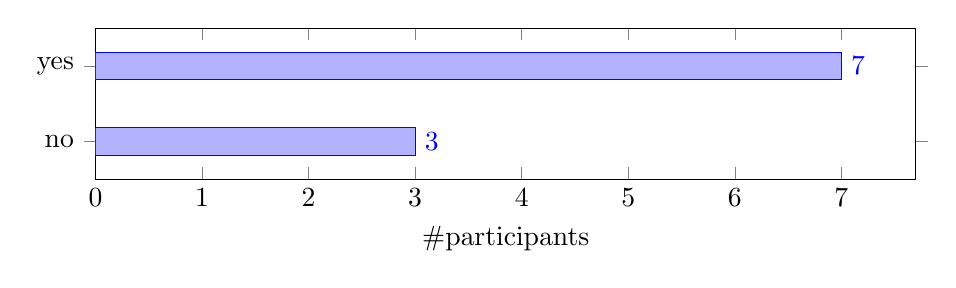
\begin{tikzpicture}
  \begin{axis}[
    xbar,
    width=12cm,
    height=3.5cm,
    enlarge y limits=0.5,
    xlabel={\#participants},
    xmin=0,
    symbolic y coords={no,yes},
    ytick=data,
    nodes near coords,
    nodes near coords align={horizontal},
    ]
    \addplot coordinates {(3,no) (7,yes)};
  \end{axis}
\end{tikzpicture}

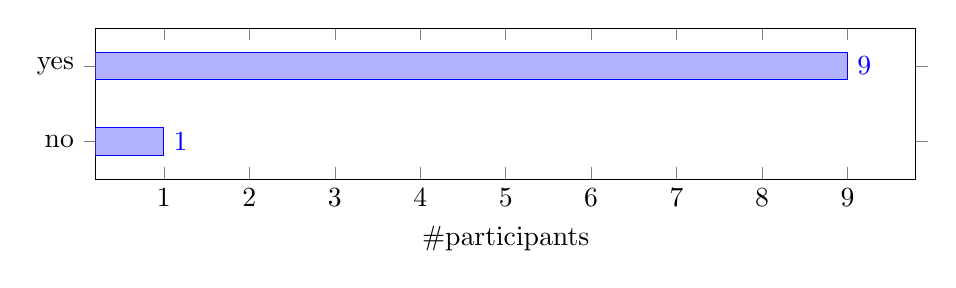
\begin{tikzpicture}
  \begin{axis}[
    xbar,
    width=12cm,
    height=3.5cm,
    enlarge y limits=0.5,
    xlabel={\#participants},
    symbolic y coords={no,yes},
    ytick=data,
    nodes near coords,
    nodes near coords align={horizontal},
    ]
    \addplot coordinates {(1,no) (9,yes)};
  \end{axis}
\end{tikzpicture}

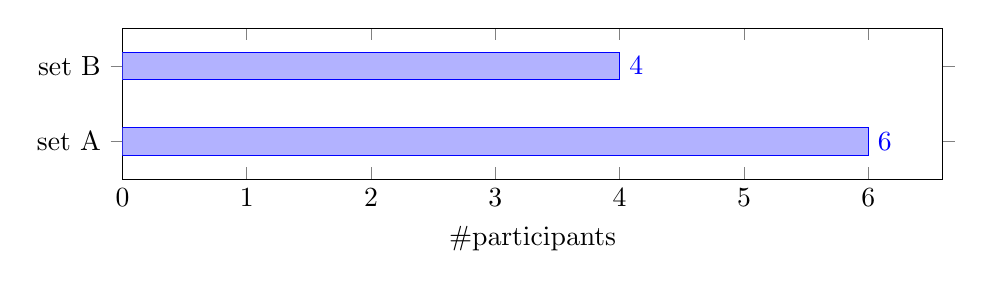
\begin{tikzpicture}
  \begin{axis}[
    xbar,
    width=12cm,
    height=3.5cm,
    enlarge y limits=0.5,
    xlabel={\#participants},
    xmin=0,
    symbolic y coords={set A,set B},
    ytick=data,
    nodes near coords,
    nodes near coords align={horizontal},
    ]
    \addplot coordinates {(6,set A) (4,set B)};
  \end{axis}
\end{tikzpicture}

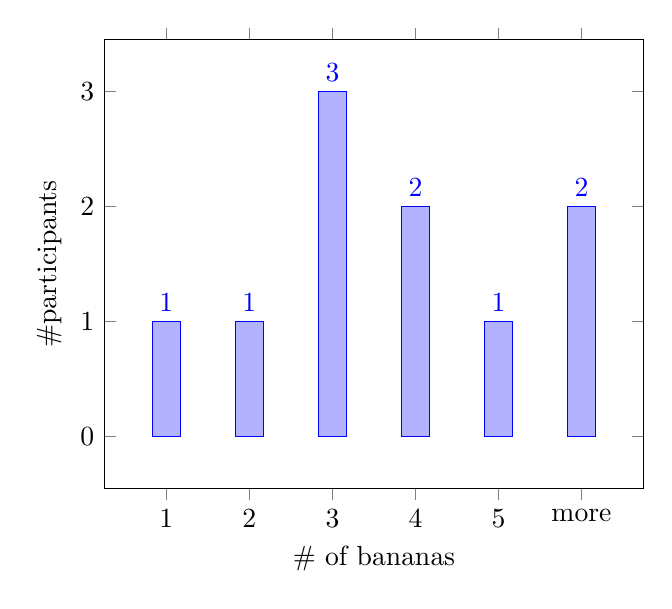
\begin{tikzpicture}
  \begin{axis}[
    ybar,
    enlargelimits=0.15,
    xlabel={\# of bananas},
    ylabel={\#participants},
    ytick={0,1,2,3},
    ymin=0,
    symbolic x coords={1,2,3,4,5,more},
    nodes near coords,
    ]
    \addplot coordinates {(1,1) (2,1) (3,3) (4,2) (5,1) (more,2)};
  \end{axis}
\end{tikzpicture}

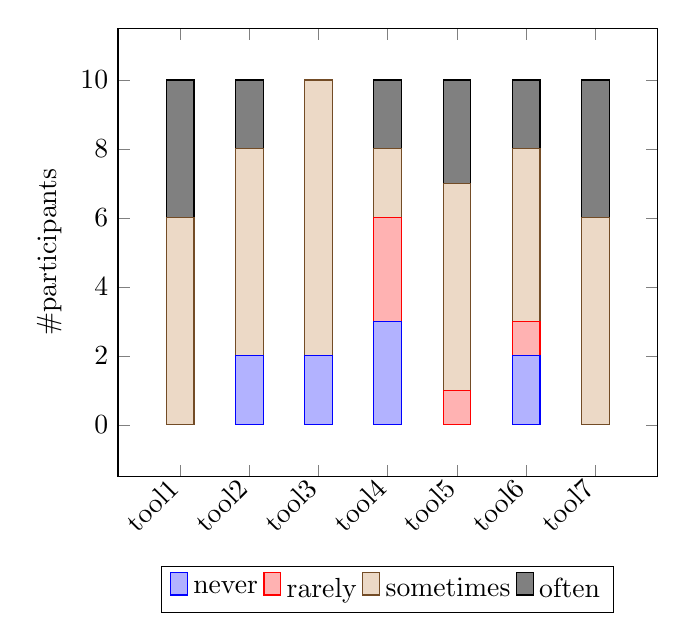
\begin{tikzpicture}
  \begin{axis}[
    ybar stacked,
    enlargelimits=0.15,
    legend style={at={(0.5,-0.20)},
      anchor=north,legend columns=-1},
    ylabel={\#participants},
    symbolic x coords={tool1, tool2, tool3, tool4, tool5, tool6, tool7},
    xtick=data,
    x tick label style={rotate=45,anchor=east},
    ]
    \addplot+[ybar] plot coordinates {(tool1,0) (tool2,2) (tool3,2) (tool4,3) (tool5,0) (tool6,2) (tool7,0)}; % never
    \addplot+[ybar] plot coordinates {(tool1,0) (tool2,0) (tool3,0) (tool4,3) (tool5,1) (tool6,1) (tool7,0)}; % rarely
    \addplot+[ybar] plot coordinates {(tool1,6) (tool2,6) (tool3,8) (tool4,2) (tool5,6) (tool6,5) (tool7,6)}; % sometimes
    \addplot+[ybar] plot coordinates {(tool1,4) (tool2,2) (tool3,0) (tool4,2) (tool5,3) (tool6,2) (tool7,4)}; % often
    \legend{never, rarely, sometimes, often}
  \end{axis}
\end{tikzpicture}

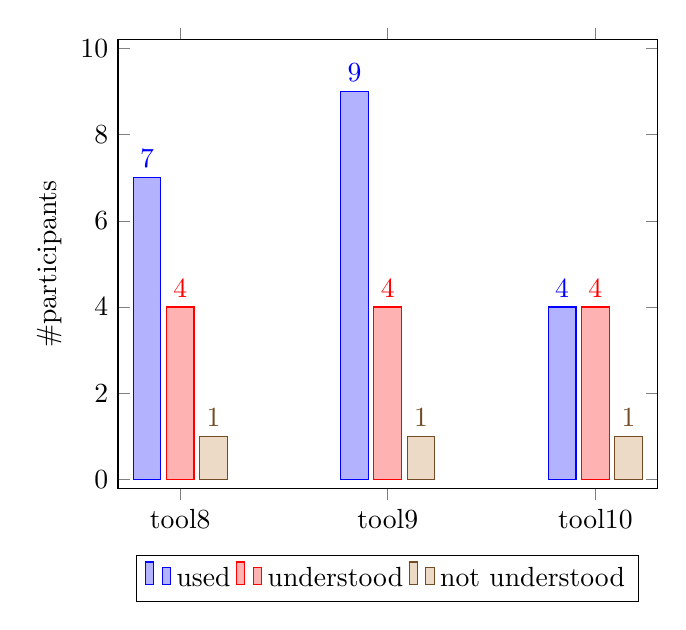
\begin{tikzpicture}
  \begin{axis}[
    ybar,
    enlargelimits=0.15,
    legend style={at={(0.5,-0.15)},
      anchor=north,legend columns=-1},
    ylabel={\#participants},
    symbolic x coords={tool8,tool9,tool10},
    xtick=data,
    nodes near coords,
    nodes near coords align={vertical},
    ]
    \addplot coordinates {(tool8,7) (tool9,9) (tool10,4)};
    \addplot coordinates {(tool8,4) (tool9,4) (tool10,4)};
    \addplot coordinates {(tool8,1) (tool9,1) (tool10,1)};
    \legend{used,understood,not understood}
  \end{axis}
\end{tikzpicture}

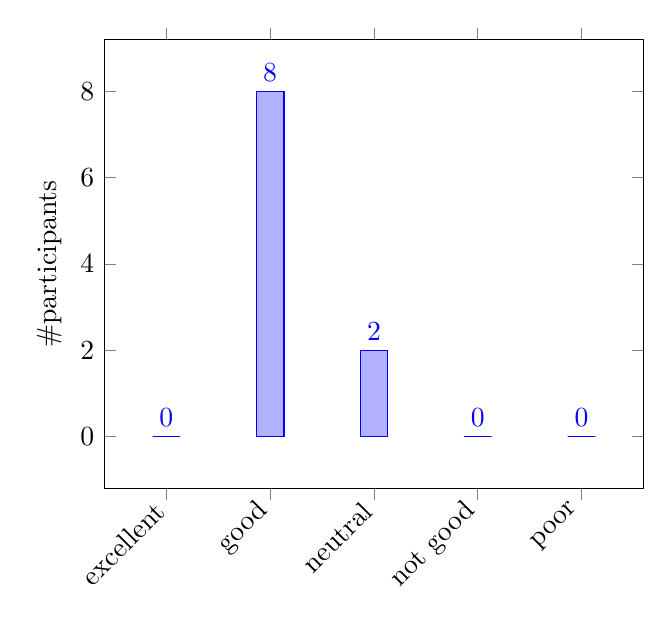
\begin{tikzpicture}
  \begin{axis}[
    ybar,
    enlargelimits=0.15,
    legend style={at={(0.5,-0.2)},
      anchor=north,legend columns=-1},
    ylabel={\#participants},
    symbolic x coords={excellent,good,neutral,not good,poor},
    xtick=data,
    nodes near coords,
    nodes near coords align={vertical},
    x tick label style={rotate=45,anchor=east},
    ]
    \addplot coordinates {(excellent,0) (good,8) (neutral,2) (not good,0) (poor,0)};
  \end{axis}
\end{tikzpicture}

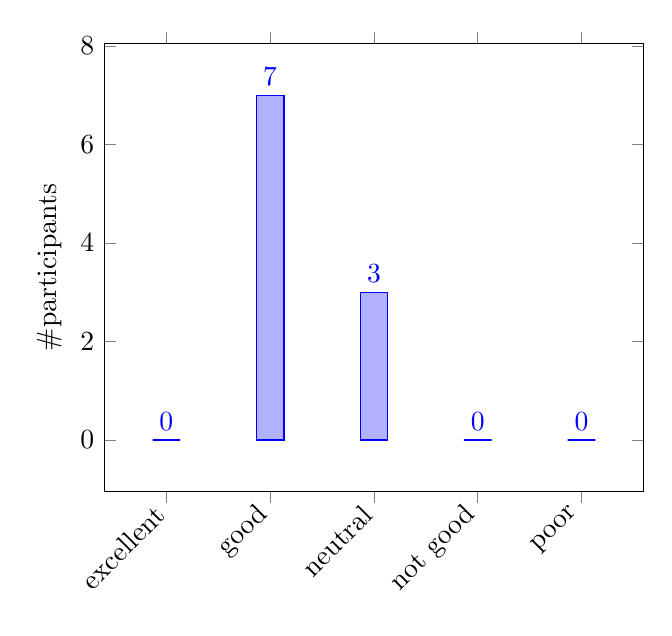
\begin{tikzpicture}
  \begin{axis}[
    ybar,
    enlargelimits=0.15,
    legend style={at={(0.5,-0.2)},
      anchor=north,legend columns=-1},
    ylabel={\#participants},
    symbolic x coords={excellent,good,neutral,not good,poor},
    xtick=data,
    nodes near coords,
    nodes near coords align={vertical},
    x tick label style={rotate=45,anchor=east},
    ]
    \addplot coordinates { (excellent,0) (good,7) (neutral,3) (not good,0) (poor,0)};
  \end{axis}
\end{tikzpicture}
\end{document}
\end{minimal}
\end{doctodo}

\begin{doctodo}[+]
  release notes:
	mention improvements of 'shader=interp'
\end{doctodo}

\begin{doctodo}[+]
  There is a typo on section 4.5.12: "As for for dimensional patch plots "
\end{doctodo}

\begin{doctodo}[+]
  quiver: the tests have a further pretty example where quiver is on top of
  a surf, attached to z =2 or so.
\end{doctodo}

\begin{doctodo}[+]
  document 'shader=faceted interp'
\end{doctodo}

\begin{doctodo}[+]
  document 'mesh/type'
\end{doctodo}

\begin{doctodo}[+]
  document the 'plot graphics/points' feature.
\end{doctodo}

\begin{doctodo}[-]
  try a bar plot with individually shaded bars 

  FIXME : collect details
\end{doctodo}

\begin{doctodo}[+]
  document 'contour prepared', 'contour external' and 'contour gnuplot'.
\end{doctodo}

\begin{doctodo}[+]
  contour external: Do not forget the \verb|\", \'| etc special handling .
\end{doctodo}

\begin{doctodo}[+]
  contour: document 'labels over line' style
\end{doctodo}

\begin{doctodo}[-]
  contour: a change label dist
\end{doctodo}

\begin{doctodo}[+]
  contour: document the special handling of "point meta".
\end{doctodo}

\begin{doctodo}[+]
  clickable: 
	document 'popup size' and its variants
	document `clickable coords size'
	document 'richtext' and the formatting things
	document \verb|\n| and friends
\end{doctodo}

\begin{doctodo}[+]
  document ternary lib
	+ do not forget 'cartesian cs' and its applications
\end{doctodo}

\begin{doctodo}[+]
  document frac whole format
\end{doctodo}

\begin{doctodo}[+]
  document /pgfplots/empty line
\end{doctodo}

\begin{doctodo}[+]
  document 'clickable coords' and 'clickable coords code' features
\end{doctodo}

\begin{doctodo}[-]
  document 'execute at begin axis' and its new variants
\end{doctodo}


\begin{doctodo}[-]
  document how to plot against the coordindex
\end{doctodo}

\begin{doctodo}[+]
  document the new 'getcolumnbyname={create col/....}' feature
\end{doctodo}

\begin{doctodo}[+]
  document linear regression 
\end{doctodo}

\begin{doctodo}[-]
  document how to identify the source of "dimension too large" errors:
  tracingstuff.
\end{doctodo}

\begin{doctodo}[+]
  document how to fix dimension too large problems: restrict to domain for
  example
\end{doctodo}

\begin{doctodo}[+]
  colorbar styles are not consistent between docs and code
\end{doctodo}

\begin{doctodo}[-]
  It seems as if the AMS command \verb|$\text{\ref{ref:to:a:plot}}$| instantiates the
  \verb|\ref| at least four times. Document somehow that it is better to use '\verb|\hbox|'
  instead
\end{doctodo}

\begin{doctodo}[+]
  pgfplotstable: show how to use '\verb|\begin{longtable}|'
\end{doctodo}

\begin{doctodo}[-]
  clickable lib:
	I have the impression that acroread fires warnings only for the manual - not always when the clickable lib is used. Why!?
\end{doctodo}

\end{bugtracker}


\section{Bugs/Features in PGF/TikZ}
\begin{bugtracker}

\begin{pgfbug}[closed]
	external lib fails if \verb|\cite[][]{dd}| is used, see MWE + workaround in \url{http://tex.stackexchange.com/questions/173465/tikz-error-for-externalized-graphics-but-output-is-correct/178684#178684} 
\end{pgfbug}

\begin{pgfbug}[closed]
	external library does not compute the shell escape flag for sub-processes correctly if run using lualatex.

	Furthermore, it would be smart to auto-detect the lualatex driver automatically
\end{pgfbug}

\begin{pgfbug}[+]
	number printer: apply 
            \verb|set thousands separator={\cdot}| also to fractional parts:
\begin{minimal}
\documentclass{article}
    \usepackage{pgf}
        \pgfset{/pgf/number format/.cd,
            set thousands separator={{{\cdot}}},
            precision=5,
        }
\begin{document}
    \pgfmathprintnumber{12345.54321}    \par
    $12 \cdot 2345.543 \cdot 21$ expected \par
\end{document}
\end{minimal}
\end{pgfbug}

\begin{pgfbug}
	When reading the manual v2.0 I found a typo 5.1 "Styling the
nodes".
Just after the first block of code, there is a sentence saying
"... can achieve them. Once way is to use ..." which should
be "One way is to use ..."

\end{pgfbug}

\begin{pgfbug}
	Beamer + pgf: the default template introduces a white line on top. Interestingly, it happens only for PGF CVS + beamer, but it appears to be dependent on third-party tools as well (see mail conversation with Stefan Tibus)
\end{pgfbug}

\begin{pgfbug}
When using externalize function together with a transform canvas, the result is somehow croped. See this example, compare output with deativated and activated externalize.
\begin{verbatim}

\documentclass{article}
\usepackage{tikz}
\usetikzlibrary{external}
\tikzexternalize % activate!
\begin{document}
\begin{tikzpicture}[transform canvas={scale=0.7}]
\node {root}
child {node {left}}
child {node {right}
child {node {child}}
child {node {child}}
};
\end{tikzpicture}
A simple image is \tikz \fill (1,0) circle(5pt);.
\end{document}
\end{verbatim}
\end{pgfbug}

\begin{pgfbug}[open]
	pgf users Vol 50 issue 6:
\begin{verbatim}
	Hi,

Thanks for TikZ.  I'm trying to use the externalization library with
the class file gOMS2e.cls, which is provided for the journal
Optimization Methods and Software.  The class file and related
files/documentation can be found here:
http://www.tandf.co.uk/journals/authors/gomslatex.zip

My problem is that the externalized figures are shifted up and to the
left significantly, cutting them off.  This problem does not occur
when not using externalization.
This seems to be related to the problem discussed here:
http://sourceforge.net/tracker/index.php?func=detail&aid=3037831&group_id=142562&atid=752792
and may also be related to this one:
http://sourceforge.net/mailarchive/forum.php?thread_name=4C0F342B.5040008%40ins.uni-bonn.de&forum_name=pgf-users

In the other cases, the solution was to use \tikzifexternalizing for
whatever conflicts with the externalization, but it seems that I can't
do this when my class file is the offending bit.  Is this true?  I
would really like to be able to use the correct \documentclass to
generate the figures so that the size/fonts/etc. are consistent
throughout the resulting document.

A minimal test example is included at the end of this message.  It
appears that the image is shifted ~1.25cm to the left and ~0.8cm up.
The problem goes away when using \documentclass{article}.
I'm using the CVS version of pgf, and I get the same result when I
produce postscript figures by using latex and setting
 \tikzset{external/system call={
   latex \tikzexternalcheckshellescape -halt-on-error
-interaction=batchmode -jobname "\image" "\texsource";
   dvips -o "\image".ps "\image".dvi}}

%----------------------------------------------------------------------------------
\documentclass[printer]{gOMS2e}
\usepackage{tikz}
\usetikzlibrary{external}
\tikzexternalize
\begin{document}
\begin{center}
  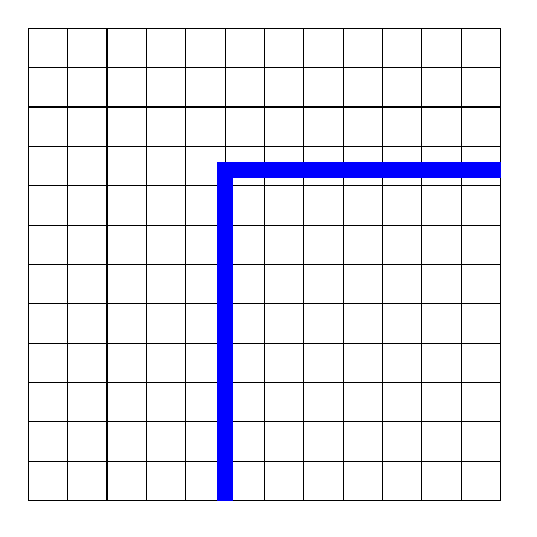
\begin{tikzpicture}
    \draw[step=.5cm] (-3,-3) grid (3,3);
    \draw[blue,line width=2mm] (-0.5,-3) -- (-0.5,1.2) -- (3,1.2);
  \end{tikzpicture}
\end{center}
\end{document}
%----------------------------------------------------------------------------------

Any help would be appreciated; I'm afraid it's over my head at this point.
Thanks!
\end{verbatim}

\end{pgfbug}

\begin{pgfbug}[closed]
	\verb|\pgfmathdivide@{-0.8}{1.00002}\pgfmathresult| yields

	\makeatletter
	\pgfmathdivide@{-0.8}{1.00002}\pgfmathresult

	instead of -0.8
\end{pgfbug}

\begin{pgfbug}
\begin{verbatim}
\documentclass{article}
\usepackage{german}
\usepackage[utf8]{inputenc} % erlaubt direkte Nutzung von Umlauten

\usepackage{pgfplots} % fuer plots

\usepackage{pgfplotstable} % fuer numeriktabellen
\usepackage{array,colortbl,booktabs}
\usetikzlibrary{external}
\tikzexternalize[force remake]

% DOESN'T WORK. Needs to disable externailization
\usepackage{vmargin}
\setpapersize{A4}
\setmarginsrb{2.5cm}{1cm}{2cm}{2cm}{8mm}{15mm}{5mm}{15mm}

\begin{document}
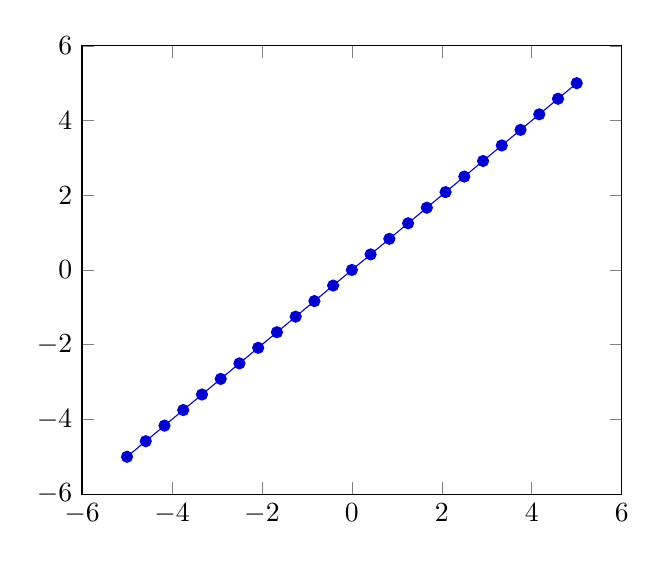
\begin{tikzpicture}
%\tracingmacros=2 \tracingcommands=2
	\begin{axis}
		\addplot {x};
	\end{axis}
\end{tikzpicture}
\end{document}
\end{verbatim}
\end{pgfbug}
\begin{pgfbug}[+]
	Implement support for space trimming and empty entries in \verb|\usetikzlibrary| and its variants
\end{pgfbug}

\begin{pgfbug}[-]
  external bug: 
\begin{verbatim}
\documentclass[
    pagesize=auto,                  % 1
        ]{scrbook}
\usepackage{tikz}
    \usetikzlibrary{external}
        \tikzexternalize
\begin{document}
        \KOMAoption{twoside}{semi}  % 2
            test
    \tikz \draw (0,0) circle (3pt);
\end{document}
\end{verbatim}
\end{pgfbug}

\begin{pgfbug}[-]
  consider a matrix style which applies only to the outer matrix node style
  (see feature request
  \verb|https://sourceforge.net/tracker/?func=detail&atid=1060657&aid=3019259&group_id=224188|
  )
\end{pgfbug}

\begin{pgfbug}[-]
  make assignments to \verb|\pgf@x| and \verb|\pgf@y| always \verb|\global|
\end{pgfbug}

\begin{pgfbug}[-]
  implement \verb|\pgfmathfloattocount|
\end{pgfbug}

\begin{pgfbug}[+]
  external lib: think whether it is possible to provide the real jobname
  without explicit user input. Idea: transport it as TeX code argument to pdflatex
\end{pgfbug}

\begin{pgfbug}[+]
  provide '$\times$' or more general formatting rules to number printer
\end{pgfbug}

\begin{pgfbug}[+]
  code 2 args doesn't work correctly with spaces between the arguments!?
\end{pgfbug}


\begin{pgfbug}[+]
  external lib: implement \verb|\tikzpicturedependsonfile#1|
\end{pgfbug}

\begin{pgfbug}[+]
  in pgfplots: invoke \verb|\tikzpicturedependsonfile|. 
  perhaps the plot-from-table-struct should also use it.
\end{pgfbug}

\begin{pgfbug}[+]
  external lib: 'list and make' does not work together with \verb|\include| (aux files!) or other file writing things -- at least not if one tries to do that in parallel.
\end{pgfbug}

\begin{pgfbug}[+]
  consider the "plot function" patch from Andy Schlaikjer
\end{pgfbug}

\begin{pgfbug}[+]
  it seems fadings don't work correctly with externalization!? 
\end{pgfbug}

\begin{pgfbug}[+]
  include addition of Christophe Jorssen for MD5 checksums in external lib
\end{pgfbug}

\begin{pgfbug}[+]
  write new sub-package 'pgfmanual.sty' which contains a good user interface to the manual styles, environments and all that.
\end{pgfbug}

\begin{pgfbug}[+]
  external lib: catcode changes inside of pictures do not work properly.
\end{pgfbug}

\begin{pgfbug}[-]
  the fpu can't be used inside of paths. That should be fixed.
	$\leadsto$ the problem is that paths may use \verb|\pgfmath...| routines directly.
	$\leadsto$ this should work! At least with the public math macros \verb|\pgfmathadd|.
	The \verb|\pgfmathadd@| might be implemented differently.
\end{pgfbug}

\begin{pgfbug}[+]
  in the manual, the first two arguments of
  pgfqkeysactivatesinglefamilyandfilteroptions were inverted.
\end{pgfbug}

\begin{pgfbug}[+]
  some predefined filters do not process unknown options correctly
\end{pgfbug}

\begin{pgfbug}[+]
  external lib in pgf: think whether 'empty image extension' is a bug or a
  feature.
	$\leadsto$ feature of \verb|\pgfimage|! Otherwise it wouldn't be possible to provide an extension!
	$\leadsto$ bug for external lib which never uses extensions!
\end{pgfbug}

\begin{pgfbug}[closed]
  fix landscape bug (pdflscape) in external lib (PGF)
\begin{minimal}
\pdfcompresslevel=0
\documentclass{article}
\usepackage{pgfplots}
%\usepackage{lscape}
\usepackage{pdflscape}

\usetikzlibrary{external}
\tikzexternalize

\begin{document}
\begin{landscape}
La.
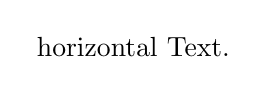
\begin{tikzpicture}
  \node at (0,0) {horizontal Text.};
\end{tikzpicture}
\end{landscape}

\end{document}
\end{minimal}
\end{pgfbug}

\begin{pgfbug}[+]
  the pgf math parser has wrong precedence for '-' prefix op:
	\verb|exp(-x^2)| is wrong.
\end{pgfbug}

\begin{pgfbug}[-,closed]
  pack the default 'system call' for dvips etc into drivers!
\end{pgfbug}

\begin{pgfbug}[-]
  active '\verb$|$' characters result in compilation bugs (\verb|\usepackage{program}|)
\end{pgfbug}

\begin{pgfbug}[-]
  'text height=1em' realisieren mit [node font units]1em 
\end{pgfbug}

\begin{pgfbug}[+]
  compatiblity code todo:
  	- the example for plot graphics (with view=0{90}) doesn't work.
	$\leadsto$ that's the '\verb|exp(0-x^2)|' bug which is still in pgf 2.00!
\end{pgfbug}

\end{bugtracker}


% BUGS
\section{Bugs in PGFPlots}

\begin{bugtracker}

\begin{bug}[-]
	histograms and density option appears to fail, compare \url{http://sourceforge.net/p/pgfplots/bugs/67/}

	and a (duplicate?) report
\begin{verbatim}
\documentclass[tikz]{standalone}
\usepackage{pgfplots}

\begin{document}
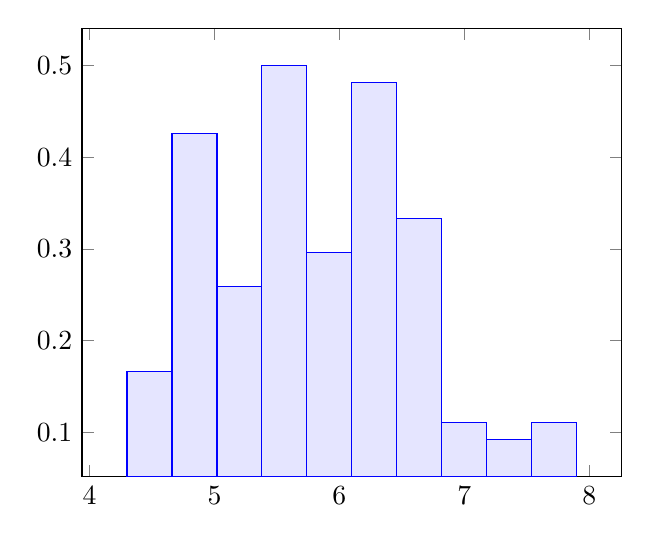
\begin{tikzpicture}
\begin{axis}\addplot+ [mark=none, fill=blue!10, hist={density}] table [row sep=\\, y index = 0] {data\\
5.1 \\ 4.9 \\ 4.7 \\ 4.6 \\ 5.0 \\ 5.4 \\ 4.6 \\ 5.0 \\ 4.4 \\ 4.9 \\ 5.4 \\ 4.8 \\ 4.8 \\ 4.3 \\ 5.8 \\ 5.7 \\ 5.4 \\ 5.1 \\ 5.7 \\ 5.1 \\ 5.4 \\ 5.1 \\ 4.6 \\ 5.1 \\ 4.8 \\ 5.0 \\ 5.0 \\ 5.2 \\ 5.2 \\ 4.7 \\ 4.8 \\ 5.4 \\ 5.2 \\ 5.5 \\ 4.9 \\ 5.0 \\ 5.5 \\ 4.9 \\ 4.4 \\ 5.1 \\ 5.0 \\ 4.5 \\ 4.4 \\ 5.0 \\ 5.1 \\ 4.8 \\ 5.1 \\ 4.6 \\ 5.3 \\ 5.0 \\ 7.0 \\ 6.4 \\ 6.9 \\ 5.5 \\ 6.5 \\ 5.7 \\ 6.3 \\ 4.9 \\ 6.6 \\ 5.2 \\ 5.0 \\ 5.9 \\ 6.0 \\ 6.1 \\ 5.6 \\ 6.7 \\ 5.6 \\ 5.8 \\ 6.2 \\ 5.6 \\ 5.9 \\ 6.1 \\ 6.3 \\ 6.1 \\ 6.4 \\ 6.6 \\ 6.8 \\ 6.7 \\ 6.0 \\ 5.7 \\ 5.5 \\ 5.5 \\ 5.8 \\ 6.0 \\ 5.4 \\ 6.0 \\ 6.7 \\ 6.3 \\ 5.6 \\ 5.5 \\ 5.5 \\ 6.1 \\ 5.8 \\ 5.0 \\ 5.6 \\ 5.7 \\ 5.7 \\ 6.2 \\ 5.1 \\ 5.7 \\ 6.3 \\ 5.8 \\ 7.1 \\ 6.3 \\ 6.5 \\ 7.6 \\ 4.9 \\ 7.3 \\ 6.7 \\ 7.2 \\ 6.5 \\ 6.4 \\ 6.8 \\ 5.7 \\ 5.8 \\ 6.4 \\ 6.5 \\ 7.7 \\ 7.7 \\ 6.0 \\ 6.9 \\ 5.6 \\ 7.7 \\ 6.3 \\ 6.7 \\ 7.2 \\ 6.2 \\ 6.1 \\ 6.4 \\ 7.2 \\ 7.4 \\ 7.9 \\ 6.4 \\ 6.3 \\ 6.1 \\ 7.7 \\ 6.3 \\ 6.4 \\ 6.0 \\ 6.9 \\ 6.7 \\ 6.9 \\ 5.8 \\ 6.8 \\ 6.7 \\ 6.7 \\ 6.3 \\ 6.5 \\ 6.2 \\ 5.9 \\ };
\end{axis}

\end{tikzpicture}
\end{document}
\end{verbatim}
	
\end{bug}

\begin{bug}[-,prio=10]
	REGRESSION: stack plots used to work for the following example (up to at least 1.8) but fail now:

\begin{verbatim}
\documentclass{standalone}

\usepackage{tikz}
\usepackage{pgfplots}
\pgfplotsset{compat=newest}

\pgfplotstableread{
1   19.178  26.027  8.219   6.849   39.726 1
2   54.795  21.918  4.110   6.849   12.329 1
3   28.767  16.438  6.849   8.219   39.726 1
4   63.014  2.740   2.740   2.740   28.767 2
5   90.411  1.370   6.849   0.000   1.370  2
6   15.068  2.740   16.438  8.219   57.534 2
7   67.123  0.000   0.000   0.000   32.877 3
8   72.603  6.849   5.479   0.000   15.068 3
9   56.164  12.329  6.849   4.110   20.548 3
10  50.685  4.110   8.219   1.370   35.616 3
}\datatable

\begin{document}
\makeatletter
\begin{tikzpicture}
\begin{axis}[
    ybar stacked
]

\addplot table[x index=0,y index=1] \datatable;
\addplot table[x index=0,y index=2] \datatable;
\addplot table[x index=0,y index=3] \datatable;
\addplot table[x index=0,y index=4] \datatable;
\addplot [stack plots=false] table[x index=0,y index=5] \datatable;
\legend{Far,Near,Here,There,NotThere}
\end{axis}
\end{tikzpicture}
\end{document}
\end{verbatim}
	
\end{bug}


\begin{bug}[prio=3]
	contour plot handler does not allow 'name path'.
\end{bug}

\begin{bug}[prio=1]
	contour plot handler does not allow to specify draw and fill -- which might be useful if just one contour is drawn/filled
\end{bug}

\begin{bug}
	REGRESSION: pgf image externalization is broken, see comments in \url{https://sourceforge.net/p/pgf/bugs/229/}
\end{bug}

\begin{bug}[closed]
	
	fill between decoration broken if set layers is active:
\begin{minimal}
\documentclass{standalone}

 \usepackage{pgfplots}
 \pgfplotsset{compat=1.10}

\usepgfplotslibrary{fillbetween}
 \begin{document}
\begin{tikzpicture}
\begin{axis}[set layers]
    \addplot[domain=0:5,
        %postaction={decorate,red,thick},
		decorate,
        decoration={
             soft clip,
             soft clip path={domain=3:5},
	 	},
    ] {x^2};
\end{axis}
\end{tikzpicture}
\end{document}
\end{minimal}


	This is active as of \verb|b7a8c0aad5a785e554d2e626c44123b0b17cf2cc|, but the bug as such is old

	I compared the input paths for the decoration for the cases set layers and no layers - they differ

	Caused by cell picture=false! This here is a reduced example:

\begin{verbatim}
\begin{tikzpicture}
	\draw (0,0) circle (5pt);
	\begin{scope}[xshift=1cm]
	\path[name path=clipper] (1.5,-1) rectangle (4,2);
    \draw[
        postaction={decorate,draw,ultra thick},
        decoration={soft clip,soft clip path={
            (1.5,-1) rectangle (4,2)
            },
        },
    ]
        (0,0) -- (1,1) -- (2,1) -- (3,0);
	\end{scope}
\end{tikzpicture}%
\end{verbatim}
\end{bug}

\begin{bug}
	pgfplots fails to handle very small number ranges on logarithmic plots (i.e. if, say, xmin and xmax are very very close to each other).

	see \url{http://www.mrunix.de/forums/showthread.php?76399-tikz-PGFplots-Fehler-dimension-too-large&p=358818#post358818}
\end{bug}

\begin{bug}
	3d axes  and y dir = reverse seems to corrupt the z ordering, see \url{http://texwelt.de/wissen/fragen/6131/pgfplots-3d-oberflachenproblem}


\end{bug}

\begin{bug}
	ybar interval  does not work well with nodes near coords

	ybar interval has an artifical last coordinate.  This will also receive nodes near coords.

	See \url{http://tex.stackexchange.com/questions/181061/pgfplots-clipping-everything-outside-a-specific-area}

\end{bug}

\begin{bug}
	ybar interval + nodes nears coords: nodes are displaced.

	The shift does not work here.
\end{bug}

\begin{bug}
	Coordinate filtering + error bars do not work.

	Expected behavior: error coordinates should be computed and coord filters should be aplied to the result. Currently, filters are evaluated first and then error coordinates.

	See \url{http://tex.stackexchange.com/questions/154084/how-to-scale-both-data-and-error-bars-in-pgfplots}
\end{bug}

\begin{bug}
	Old sampling no-go bug: \verb|\pgfplotsforeachungrouped \x in {0,1,...,5000}| is numerically instable (because I hesitated to do expensive float comparisons all the time...)

	\url{http://tex.stackexchange.com/questions/183369/tikz-and-pgfplot-problem-with-plotting}
\end{bug}

\begin{bug}
	fillbetween / intersection lib bug:
	see minimal at \url{http://tex.stackexchange.com/questions/180899/fillbetween-library-sometimes-works-and-sometimes-does-not/181224#181224}
\end{bug}

\begin{bug}
	\verb|legend to name| appears to be broken if the legend is empty (empty matrix?) TODO: verify that empty legends do not cause problems here!
\end{bug}

\begin{bug}
	cube/size x   has no effect if used in a 2d axis
\end{bug}

\begin{bug}
	copy paste from the manual does not copy empty lines --- which is quite bad for the 3d surface examples

	This appears to be a known issue for pdf, with few available work-arounds.
	The listings package suffers from it as well (at least regarding trailing spaces/tabs); there are a couple of related questions at tex.sx

	A way might be to use \verb|\usepackage{accsupp}| with something like
\begin{verbatim}
\documentclass{article}

\usepackage{accsupp}

\begin{document}
\long\def\XXX{A 
	^^J
  ^^J
B}
\BeginAccSupp{method=escape,ActualText=\XXX}
First line

second line
\EndAccSupp{}

\end{document}
\end{verbatim}
	Expected result: copy-pasting that segment should yield A (newline) B. But it does not work with newlines as it seems

	One entry on tex.sx mentioned that Microsoft products can insert empty lines in copy-paste output (suggested solutions there was to generate such a pdf and include it as graphics unless I am mistaken)


	I managed to get this up and running so far -- but the result is unusable! both acrobat and xpdf get utterly confused unless one hits exactly on some invisible lines
\begin{minimal}
\pdfcompresslevel=0
\documentclass{article} 
\usepackage{pgfplots}
\usepackage{accsupp}
\pgfplotsset{compat=1.7}

\begin{document}

Test before

\begingroup
\catcode`\ =12\relax%
\catcode`\^^M=13\relax%
\def^^M{^^J}%
\def\begin{\string\begin}%
\def\end{\string\end}%
\def\addplot{\string\addplot}%
\xdef\copypastable{%
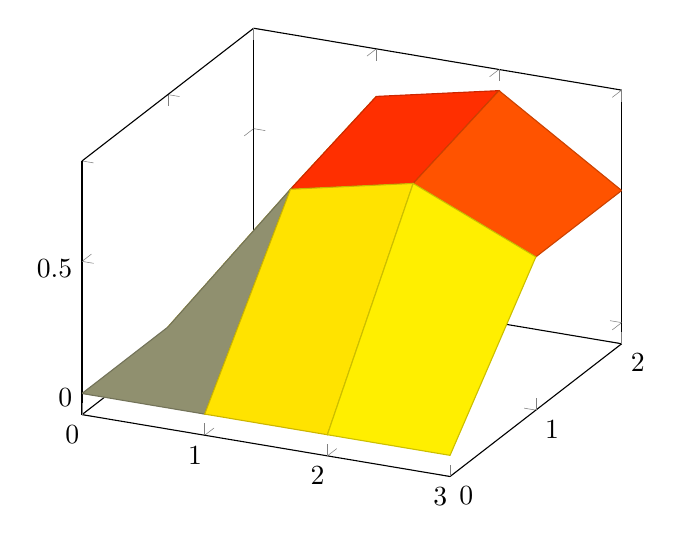
\begin{tikzpicture}
    \begin{axis}
        \addplot3[surf] coordinates {
            (0,0,0) (1,0,0)   (2,0,0)   (3,0,0)

            (0,1,0) (1,1,0.6) (2,1,0.7) (3,1,0.5)

            (0,2,0) (1,2,0.7) (2,2,0.8) (3,2,0.5)
        };
    \end{axis}
\end{tikzpicture}%
}\endgroup

\BeginAccSupp{%
		method=escape,%
		ActualText={\copypastable}}
\begin{verbatim}
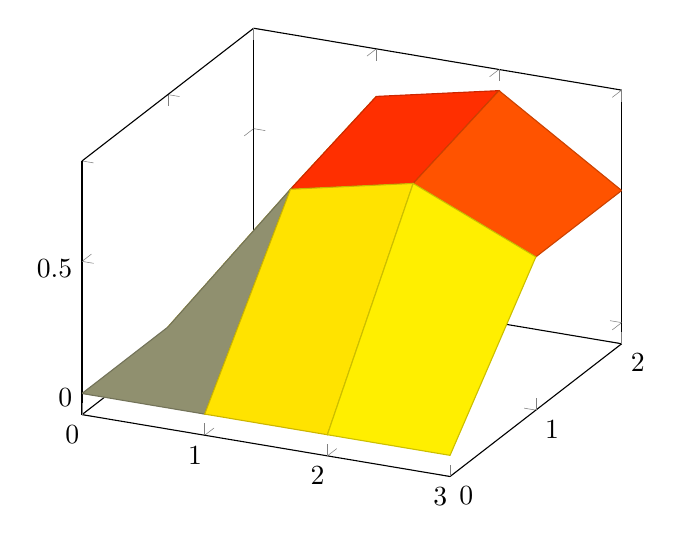
\begin{tikzpicture}
    \begin{axis}
        \addplot3[surf] coordinates {
            (0,0,0) (1,0,0)   (2,0,0)   (3,0,0)

            (0,1,0) (1,1,0.6) (2,1,0.7) (3,1,0.5)

            (0,2,0) (1,2,0.7) (2,2,0.8) (3,2,0.5)
        };
    \end{axis}
\end{tikzpicture}
\end{verbatim}
\EndAccSupp{}%

Text middle

\begingroup
\catcode`\ =12\relax%
\catcode`\^^M=13\relax%
\def^^M{^^J}%
\def\begin{\string\begin}%
\def\end{\string\end}%
\def\addplot{\string\addplot}%
\xdef\copypastable{%
\begin{tikzpicture}
    \begin{axis}[small,view={0}{90}]
    \addplot3[surf,shader=interp,patch type=bilinear,
        mesh/color input=explicit]
    coordinates {
        (0,0,0) [color=blue] (1,0,0) [color=green]

        (0,1,0) [color=yellow] (1,1,1) [color=red]
    };
    \end{axis}
\end{tikzpicture}
}\endgroup

\BeginAccSupp{%
		method=escape,%
		ActualText={\copypastable}}
\begin{verbatim}
\begin{tikzpicture}
    \begin{axis}[small,view={0}{90}]
    \addplot3[surf,shader=interp,patch type=bilinear,
        mesh/color input=explicit]
    coordinates {
        (0,0,0) [color=blue] (1,0,0) [color=green]

        (0,1,0) [color=yellow] (1,1,1) [color=red]
    };
    \end{axis}
\end{tikzpicture}
\end{verbatim}
\EndAccSupp{}%

Text after
\end{document}
\end{minimal}
	Problems here:
	\begin{itemize}
		\item one has to mark the right segments, and these can only be found by trial and error
		\item hitting the wrong one will copy nothing or only parts
		\item in the manual, I often had the wrong content in my clipboard (some older state of the clipboard, no idea where that came from)
	\end{itemize}
\end{bug}

\begin{bug}
	tikz intersections: the ``store in macro'' methods do not use global macros. Should they!? 
\end{bug}

\begin{bug}
	fill between: 
\verb|addplot [draw=green!80,fill=green!20] fill between [of=lower and axis, soxft clip={(intersection-\numintersections) rectangle (axis cs:\pgfkeysvalueof{/pgfplots/xmax},0)}]|

 	produces no ``unknown key soxft clip'' error
\end{bug}

\begin{bug}
	fill between / intersections lib bug: spurious intersections \url{http://tex.stackexchange.com/questions/180127/stacking-plots-in-animation-using-fill-between-library-with-dynamic-calculation/180299#180299}

	analysis in \verb|~/tmp/bug_intersectionlibs.tex|: problem seems to be the duplicate detection

	problem: almost parallel lines:
\begin{verbatim}
\begin{tikzpicture}
	\makeatletter
	 \def\A{%
	 	\pgfsyssoftpath@movetotoken{15.60165pt}{0.60783pt}%
		\pgfsyssoftpath@linetotoken{0pt}{0pt}%
	}%
	 \def\B{%
	 	\pgfsyssoftpath@movetotoken{15.60165pt}{0.81604pt}%
		\pgfsyssoftpath@linetotoken{0.0pt}{0.33199pt}%
	}%
	\draw[blue] \pgfextra{\pgfsetpathandBB\A};
	\draw[red] \pgfextra{\pgfsetpathandBB\B};
    \pgfintersectionofpaths%
        {%
          \pgfsetpath\A
        }%
        {%
          \pgfsetpath\B
        }%

	\pgfmathloop%
	\ifnum\pgfmathcounter>\pgfintersectionsolutions\relax%
	\else%
	\draw[red] \pgfextra{\pgftransformshift{\pgfpointintersectionsolution{\pgfmathcounter}\message{\pgfmathcounter=(\the\pgf@x,\the\pgf@y)^^J}}}%
	node[anchor=center] {\pgfmathcounter/\pgfintersectionsolutions};
	\repeatpgfmathloop%

	 \end{tikzpicture}
\end{verbatim}
\end{bug}

\begin{bug}
	pgfplotstable appears to have problems with \verb|#| in col names, compare  \url{http://tex.stackexchange.com/questions/175395/how-can-csv-files-be-put-into-latex-without-having-to-adjust-much}
\end{bug}

\begin{bug}[closed] % REJECT THIS. WON'T FIX
	\verb|shader=interp| seems to use a different way to generate triangles compared to \verb|shader=faceted|, compare
\begin{verbatim}
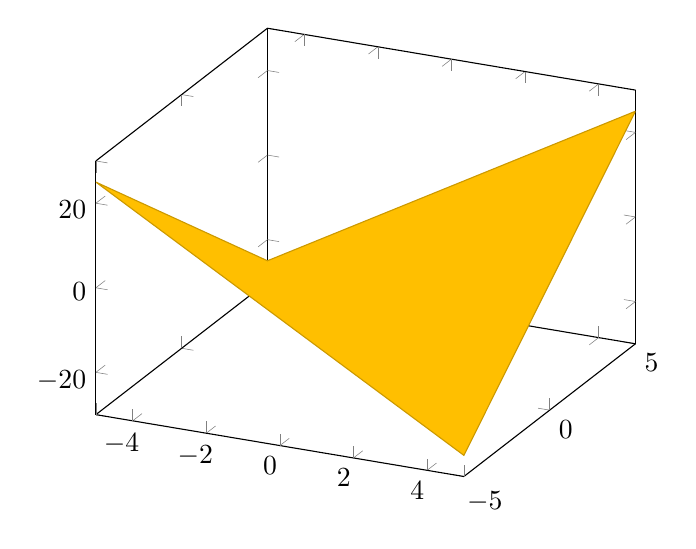
\begin{tikzpicture}
	\begin{axis}
	\addplot3[surf,samples=2] {x*y};
	\end{axis}
\end{tikzpicture}
	
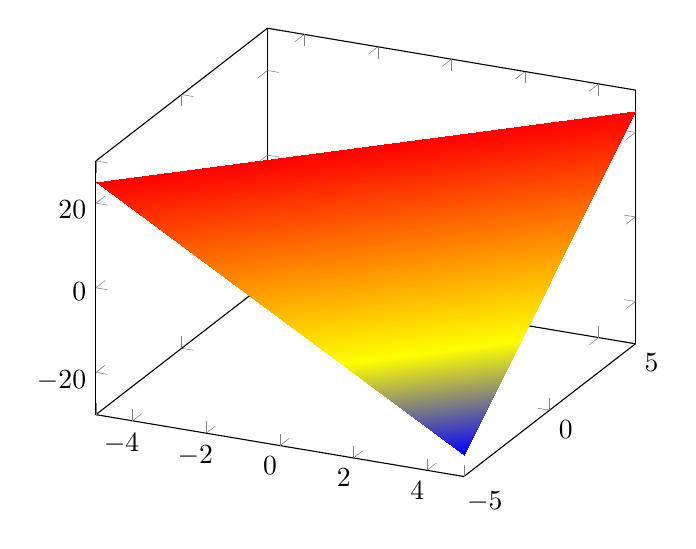
\begin{tikzpicture}
	\begin{axis}
	\addplot3[surf,samples=2,shader=interp] {x*y};
	\end{axis}
\end{tikzpicture}
\end{verbatim}
\end{bug}

\begin{bug}[closed]
	Using mesh legends with \verb|shader=interp| causes a wrong bounding box for the legend image
\begin{verbatim}
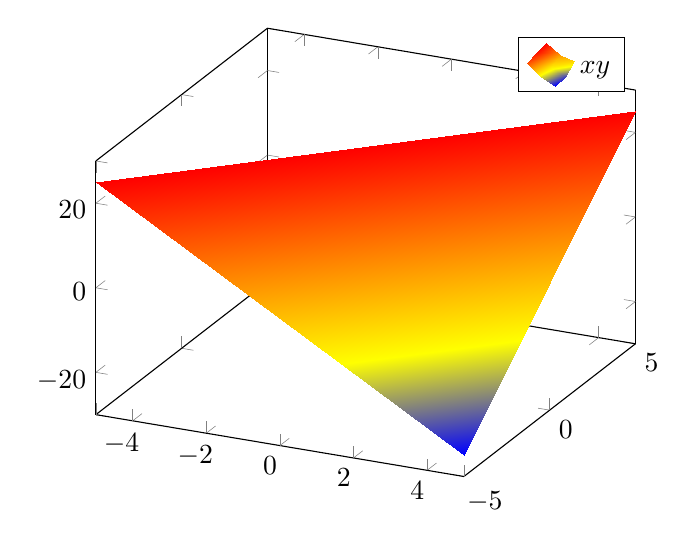
\begin{tikzpicture}
	\begin{axis}[legend entries=$xy$]
	\addplot3[surf,samples=2,shader=interp] {x*y};
	\end{axis}
\end{tikzpicture}
\end{verbatim}

\begin{minimal}
\pdfcompresslevel=0
\pdfminorversion=4
\documentclass{standalone}

\usepackage{pgfplots}

\begin{document}
\makeatletter
\fbox{%
		\tikzpicture
			\pgfplotsplothandlermesh@defaultlegend@img{%
				/pgfplots/shader=interp,
				% undo some shift hard-coded in the macro:
				%yshift=0.7cm,%
				%
				% this repairs it!
				%scale=1/0.4,
			}%
		\endtikzpicture
}%
\end{document}
\end{minimal}
\end{bug}

\begin{bug}[+]
	fillbetween configures set layers - but this does not really take effect, see

	\url{http://tex.stackexchange.com/questions/170967/pgfplots-grid-lines-below-filling/171100#171100}

\end{bug}

\begin{bug}[prio=2]
	context + color mix produces spurious shifts
\begin{verbatim}
I'm using pgfplots to create some bar charts with error bars in ConTeXt,
and I want to use custom colours for them.  This works, but if I mix a
custom colour with another colour, it results in a gap between the
error bar line and the error bar mark.  If two custom colours are
mixed, the gap seems to be doubled.  Mixing with predefined colours
works normally.  MWE:

\usemodule[tikz]
\usemodule[pgfplots]

\definecolor	[Blue]	[h=3465a4]
\definecolor	[White]	[h=ffffff]

\pgfplotsset{compat=newest}

\starttext
\starttikzpicture
	\startaxis[ybar, error bars/y dir=both, error bars/y explicit]
		\addplot+[blue!50!white] coordinates {(1,5) +- (0,3)};
		\addplot+[Blue] coordinates {(1,5) +- (0,3)};
		\addplot+[Blue!50!white] coordinates {(1,5) +- (0,3)};
		\addplot+[Blue!50!White] coordinates {(1,5) +- (0,3)};
	\stopaxis
\stoptikzpicture
\stoptext

Here you can see the result:
http://666kb.com/i/cl86t0mfpin35tht7.png
\end{verbatim}
\end{bug}


\begin{bug}[+]
	3d centered axis lines: tick lines are drawn incompletely

	See
\begin{minimal}
\documentclass[tikz,12pt]{standalone}
\usepackage{tikz,pgfplots,pgfplotstable}

\pgfplotsset{compat=newest}

\begin{document}
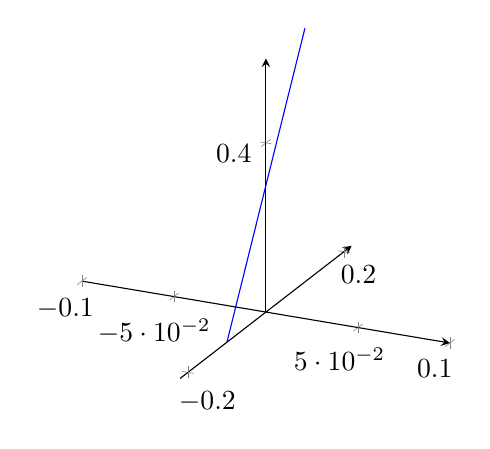
\begin{tikzpicture}

%\pgfplotsset{every axis/.append style={tick style={line width=0.7pt}}}

\pgfplotstableread{
a b
-0.1 0.2
0.1 0.5
}\testdata

\begin{axis}[axis lines=center, ymin=-0.22,ymax=0.22,xmin=-0.1,xmax=.1  ]
    \addplot3 [color=blue,] table[x expr=0,y=a,z=b] {\testdata};
\end{axis}

\end{tikzpicture} 
\end{document}
\end{minimal}
\end{bug}

\begin{bug}[closed]
	\verb|\addplot graphics| internally tries to use \verb|\includegraphics| even on ConTeXt

this can be fixed by defining

\verb|\def\includegraphicscompat[#1]#2{\externalfigure[#2][#1]}|

and setting

\verb|includegraphics cmd=\includegraphicscompat|

on ConTeXt. It should be done by PGF Plots automatically
\end{bug}

\begin{bug}[closed]
	patchplots lib: legends fail to compile for nonstandard patch types

	add a legend to \url{http://tex.stackexchange.com/questions/166570/color-and-legend-for-3d-surface}
\end{bug}

\begin{bug}[closed]
	surf legends have broken bounding boxes when used with an interpolated shading

	add a legend to \url{http://tex.stackexchange.com/questions/166570/color-and-legend-for-3d-surface} and fix the other related bug
\end{bug}

\begin{bug}[closed]
	fill between: the path commands before the semicolon in \verb|\addplot fill between [] ;| are ignored/unsupported.
\end{bug}

\begin{bug}[prio=3]
	fill between: \verb|soft clip={domain=1:2}}| might fail if the function in question touches the y boundary within the domain. In this case, the soft clip path produces unwanted side--effects.

	Cure: enlarge the soft clip path generated by \verb|domain|. It should be bigger than the function in question (with respect to $y$)

	(I have a not-quite-minimal example in my tmp folder)
\end{bug}

\begin{bug}[closed]
	fill between: (in fact, it is just pure tikz) Adding pins after the main path affects the name path:
\begin{minimal}
\documentclass{standalone}
    \usepackage{tikz}
    \usepackage{pgfplots}

	\usepgfplotslibrary{fillbetween}
\begin{document}

\begin{tikzpicture}
    \begin{axis}[smooth]

        % ... (der letzte) Pins jedoch schon
        % (beim Tauschen der 'pos'-Werte verursacht weiterhin der letzte das Problem)
        \addplot+[name path=A] table [x=x,y=y] {
x y z
0 2 3
0.5 -1 0
1 3 4
		}
        %    node [coordinate,pos=0.9, pin=above right:test] {}
            node [coordinate,pos=0.1, pin=above right:test] {}
        % folgt dem Pin noch ein Label, hat dieses keinen Einfluss
         %   node [pos=0.8] {blub}
        ;

		\addplot+[name path=B,domain=0:1,samples=2] {0};

		\addplot fill between[of= A and B];
    \end{axis}
\end{tikzpicture}
\end{document}
\end{minimal}
\end{bug}

\begin{bug}[prio=2]
	Adding user decorations to axis lines might interfer with the discontinuities which are also decorations, compare 

	\url{http://tex.stackexchange.com/questions/160936/random-decoration-of-plot-axis-messes-up-direction-of-axis-arrow/161025#comment368659_161025}

	I already added Jake's workaround to the code, but might still need more cleanup (and for non-centered axis lines as well)
\end{bug}

\begin{bug}[prio=4]
	adding a post action with decoration to a pgfplots style results in an error if markers are active 
\end{bug}

\begin{bug}[prio=3]
	Usability issues around histograms: \url{http://tex.stackexchange.com/questions/151411/histogram-frequention-polygon/151551#151551}

\begin{minimal}
\documentclass{standalone}
\usepackage{tikz}
\usetikzlibrary{calc,intersections,through,backgrounds,snakes}
\usepackage{pgfplots}
\pgfplotsset{compat=1.8}
\usepgfplotslibrary{statistics}
\begin{document}
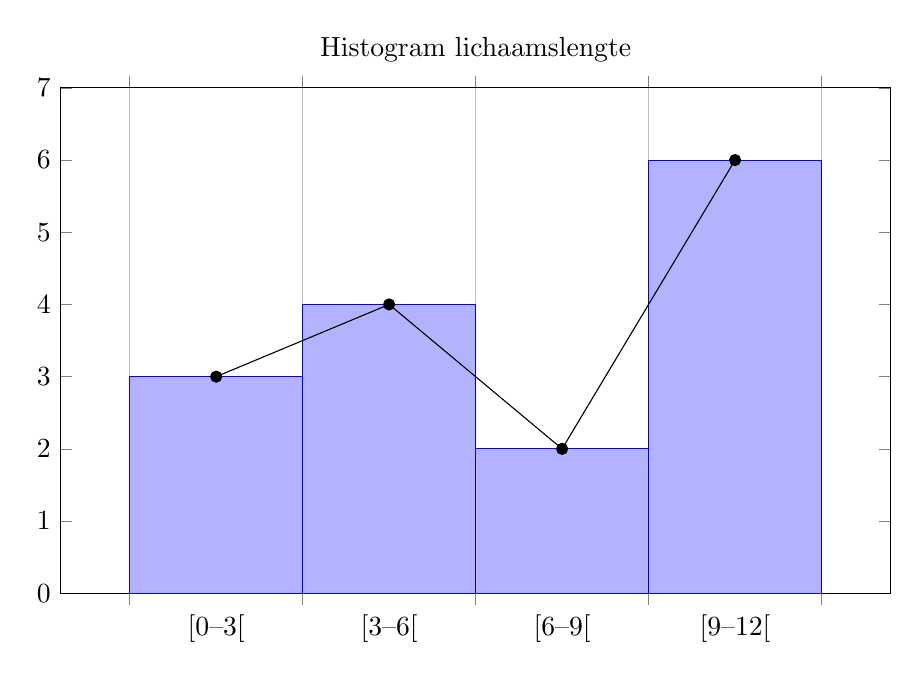
\begin{tikzpicture}
\begin{axis}[
width=1*\textwidth,
height=8cm,
ymin=0,
ymax=7,
title=Histogram lichaamslengte,
ybar interval,
xticklabel={[\pgfmathprintnumber\tick--\pgfmathprintnumber\nexttick [}],
\addplot+[hist={bins=4, data max=12,data min=0}]
table[row sep=\\,y index=0] {
data\\
1\\ 2\\ 1\\ 5\\ 4\\ 10\\ 4\\ 5\\ 7\\ 10\\ 9\\ 8\\ 9\\ 9\\ 11\\
};

\addplot[
	%
	% there seems to be a bug in pgfplots which would shift the two
	% 'hist' plots as if both were bar plots.
	% This is one possible work-around:
	forget plot,
	%
	mark=*,
	hist={bins=4, data max=12,data min=0,
		% this here should *not* become an ybar interval:
		handler/.style={sharp plot},intervals=false,
	},
	%
	% .. but since the other plot is shown with intervals, we should
	% shift this here accordingly:
	shift={(axis direction cs:1.5,0)},
]
table[row sep=\\,y index=0] {
data\\
1\\ 2\\ 1\\ 5\\ 4\\ 10\\ 4\\ 5\\ 7\\ 10\\ 9\\ 8\\ 9\\ 9\\ 11\\
};
\end{axis}
\end{tikzpicture} 
\end{document}
\end{minimal}
	
	Problems: 
	\begin{itemize}
		\item point meta uses the wrong values (try out nodes near coords)
		\item ybar interval is active for the second plot
		\item interval=false should be deduced automagically
	\end{itemize}

\end{bug}

\begin{bug}[prio=2]
	Loading a pgfplots library via \verb|\usetikzlibrary{pgfplots...}| fails unless pgfplots is loaded. This should be reported properly (or perhaps load pgfplots implicitly?)
\end{bug}

\begin{bug}[prio=1]
	The special feature \verb|patch,patch type=quadratic spline, point meta=none| which produces global paths appears to duplicate the low level path. I suppose this can only be seen in the resulting pdf file or in a debugger, but it makes a big difference when used together with decorations or fill between.

	This feature should be documented in more places as well.

	FOUND IT: the problem is stated incorrectly: the path is generated once (and only once). BUT: \verb|\tikz@mode| is invoked twice, once by the mesh plot handler and once by tikz. This is idempotent, in general -- but not if we have \verb|name path=A| in place! In this case, the softpath will be \emph{appended} every time \verb|\tikz@mode| is being executed.

	INACTIVE: at the time of this writing, the offending ``append'' feature of \verb|name path| is inactive; this bug does not happen anymore 
\end{bug}

\begin{bug}[closed]
	stacked plots with empty increments but errors bars broke in 1.9:
\url{http://tex.stackexchange.com/questions/150243/pgfplotssetcompat-1-9-causes-y-0-error-bar-to-disappear}
\end{bug}

\begin{bug}[closed]
	color space selection does not apply to colorbars. To this end, one would need to install
\begin{verbatim}
		% workaround for a weakness of PGF: PGF does not support non-RGB
	% shadings. But shader=interp does:
	colorbar sampled={surf,shader=interp},
	%
	% 'colorbar sampled' reconfigures styles and sets colorbar=true.
	% Set it back:
	colorbar=false,
\end{verbatim}
	in the ``correct'' environment (probably at begin document)
\end{bug}

\begin{bug}[prio=1]
	\verb|\usepackage[gray]{xcolor}| does not seem to work as good as for cmyk... in particular, the default color map is not being converted correctly!? Probably because xcolor does not convert the colors if they are RGB

		This appears to be irrelevant because RGB gray colors can be translated losslessy to scalar gray values!?
\end{bug}

\begin{bug}[closed]

	Successive use of \verb|\pgfplotstablenew| appears to rely on old results, compare \url{http://tex.stackexchange.com/questions/148820/repeated-pgfplotstable-calls-causing-errors}
\end{bug}

\begin{bug}[prio=2]
	some issue regarding extra ticks in log axes has been reported in \url{http://tex.stackexchange.com/questions/148703/bug-pgfplots-extra-ticks}
\end{bug}

\begin{bug}
	box plots appear to have a bug when the number of coordinates / duplicates is special: \url{http://tex.stackexchange.com/questions/146663/pgfplots-fails-to-generate-boxplots-for-some-data-set?noredirect=1#comment332779_146663}	
\end{bug}


\begin{bug}
	\url{http://tex.stackexchange.com/questions/104010/why-does-loading-pgfplots-after-tikz-break-the-default-layers-in-a-tikzpicture}
	is still active .

	Solution: backgrounds lib must be loaded after pgfplots. Apparently, the backwards layer stuff overwrites hooks of the backgrounds lib
\end{bug}

\begin{bug}[closed]
	lualatex backend does not support external lib + up to date check=md5. (only with \verb|\usepackage{pdftexcmds}|)

	add special LUA function to compute md5 sum
\end{bug}

\begin{bug}
	default tick labels are placed outside of displayed area if \verb|unit vector ratio*=1 1| is in effect

\begin{verbatim}
\documentclass{article}
\usepackage{pgfplots}
\usetikzlibrary{decorations.markings}
\pgfplotsset{compat=1.8}

\begin{document}

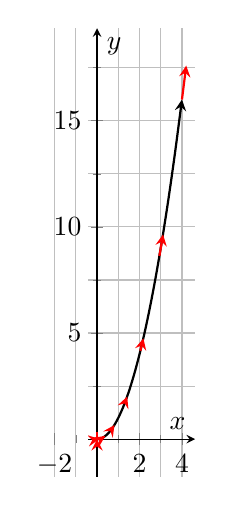
\begin{tikzpicture}
\begin{axis}[axis lines = middle,smooth,xlabel = $x$, ylabel =$y$, minor tick num =1, grid=both, unit vector ratio*=1 1,enlargelimits = true]
\addplot[smooth, thick, -stealth,variable=\t, domain=0:2, ]
	({t^2}, {t^4});

\addplot[thick, red,-stealth,samples=8,variable=\t, domain=0:2,quiver={
		u=2*t, v=4*t^3, scale arrows=0.05,
	}]
	({t^2}, {t^4});
\end{axis}
\end{tikzpicture}

\end{document}
\end{verbatim}
\end{bug}

\begin{bug}[+]
	The default setting
	\verb|plot to file/col sep/.initial=\pgfplots@TAB,|

	does fails to work in xelatex

	\url{http://tex.stackexchange.com/questions/140700/what-is-wrong-with-this-code-to-plot-y2-2-cosx}
\end{bug}

\begin{bug}
	\verb|ytick=data| does not work together with stacked plots because, by design, it merely considers coordinates of the \emph{first} plot. That's nonsense for stacked plots.
\end{bug}

\begin{bug}[prio=2]
	The combination of 3d unit vectors and \verb|scale mode=stretch to fill| is useful, but unsupported.

	I made a brief experiment to verify that it does something useful if 
	\begin{itemize}
		\item the data scaling is disabled in setunitvector
		\item the first if branch of \verb|...@prepare@plotbox@limits| is activated.
	\end{itemize}
	References: \url{http://tex.stackexchange.com/questions/139686/controlling-orientation-in-3d-pgf-plots}
\end{bug}

\begin{bug}
	Tick labels suffer from inexact arithmetics in Tikz foreach:
\begin{verbatim}
KAPUTT:

  \foreach \x in {1,1.1,...,2} {\x\par}

OK:

  \foreach \x in {1,1.1,...,2.001} {\x\par}
\end{verbatim}
\end{bug}

\begin{bug}
	ytick=data combined with minor y tick num does not work as expected: minor tick lines will be skipped below the lowest limit.
\end{bug}

\begin{bug}
	pgfplotstable does not apply \verb|postproc cell content| in \verb|every row| styles

	see \url{http://tex.stackexchange.com/questions/111492/postprocess-row-with-pgfplotstable}
\end{bug}

\begin{bug}
	no markers: it appears to be impossible to switch off markers, only for scatter plots.

	See \url{http://tex.stackexchange.com/questions/105850/pgfplots-points-with-no-marks-but-errorbars}
\end{bug}

\begin{bug}[prio=3]
	units and square brackets
\begin{verbatim}
Dann habe ich noch eine Anmerkung bzgl. der Verwendung von Einheiten in Achsbeschriftungen, Punkt "5.10 Units in Labels". Generell sehr hilfreich, allerdings möchte ich darauf hinweisen, dass die Verwendung von eckigen Klammern um Einheiten falsch und unzulässig ist. Auch wenn man es leider immer wieder (falsch) selbst in (schlechten) Lehrbüchern sieht. Indes, falsch bleibt falsch und mit diesem schlechten Usus sollte gebrochen werden. Hierzu 'DIN 1313: Größen', die Anmerkung zu Punkt 4.3

------ Zitat
ANMERKUNG;
Die eckigen Klammern dürfen nicht um Einheitenzeichen gesetzt werden. Angaben wie [kg] sind nicht zu verwenden, auch nicht zur Beschriftung von Koordinatenachsen in graphischen Darstellungen (siehe DIN 461).
------ Ende Zitat

'DIN 461: Graphische Darstellung in Koordinatensystemen' gibt Beispiele, wie es gemacht werden soll.

Hintergrund: formaler Zusammehang ist X={X}[X]. Das heißt: X=5N --> {X}=5 und [X]=N. Unsinnig ist [N] da "[...]" für "Einheit von ..." steht und was ist die Einheit einer Einheit?! Nachzulesen auch in jedem guten Physik-Lehrbuch.

Wie gesagt: leider eine sehr schlechte Angewohnheit und den meisten unbekannt oder schlicht egal. Anders ist die allzu häufige Verwendung nicht zu erklären. Deshalb sollte zumindest ein Hinweis zu lesen sein, dass diese Syntax eigentlich falsch/unzulässig ist.
\end{verbatim}
	
	While I understand the problem, I am inclined to keep it as-is... I cannot break backwarts compatibility now, and I hear few complaints. I suppose the units stuff could be reviewed at some time
\end{bug}

\begin{bug}
	\verb|...| and rounding:
	
	Generell erscheint mir die \verb|...|-Syntax nicht robust. Bei kleinen, durchaus nicht ungewöhnlichen, Intervallen kommt es zu Rundungsfehlern:

Hauptgitter:

\verb|ytick={0.99,1.00,1.01,1.02,1.03,1.04,1.05,1.06,1.07,1.08}|

Hilfsgitter:

\verb|minor ytick={0.99,0.991,...,1.08}|

Führt dazu, dass die Hilfslinien mit zunehmender Größe immer weiter von den Hauptgitterlinien verschoben sind, obwohl diese aufeinanderliegen sollten.
Mit Hilfsgitter komplett ausgeschrieben:

 \verb|minor ytick={0.99,0.991,0.992,0.993,...............,1.08}|

passt es. Die \verb|...|-Syntax ist daher absolut mit Vorsicht zu genießen.

\end{bug}

\begin{bug}
	box plots with draw direction=y and xtick=data fail to provide the correct xtick locations
\end{bug}


\begin{bug}[prio=2]
	boxplots: predefined legend entries need to be improved
\end{bug}

\begin{bug}[+]
	Bug: bounding box wrong (regression in git repo; not in stable) bisect:
\begin{verbatim}
	3ad5df8050b8c79c67d8831246387cec67ed625d is the first bad commit
commit 3ad5df8050b8c79c67d8831246387cec67ed625d
Author: Christian Feuersaenger <ludewich@users.sourceforge.net>
Date:   Tue Jan 1 21:41:19 2013 +0100

    BB is now tight if hide axis=true - independent of clip path.


reproducable:
pdflatex unittest_enlargelimits_14.tex
\end{verbatim}
\end{bug}

\begin{bug}
	presets for mark size and tiny / footnotesize are wrong
\end{bug}

\begin{bug}[+]
	regression: shader=interp can produce wrong clip regions for the shading, compile \url{http://tex.stackexchange.com/questions/91689/visualize-data-on-a-variable-radius-graph-network/93858#93858}	 to see it


	While that issue is solved, there are still BB issues which need to be fixed. In particular, the BB can extend the clip region. Solution approaches: 
	\begin{itemize}
		\item \ok compute precise BB (using necessary condition on derivative)
		\item \ok compute the pdf Xform's bounding box using the method here (i.e. the bounding box derived from control points). BUT: update the picture's BB using the interpolation points (not the control points). This is more natural anyway, and it will probably result in a correct BB. If not, the user can easily extend it.

	\end{itemize}
\end{bug}

\begin{bug}
	clipping of tick lines does not respect the line width of the axis lines.
	
	\url{http://tex.stackexchange.com/questions/91517/how-to-make-the-tick-thickness-as-the-axis-line/91645#91645}
\end{bug}

\begin{bug}
	Inf geht nicht im math parser:
\begin{verbatim}
\documentclass[a4paper]{article}

\usepackage{pgfplots}


\begin{document}

\pgfmathfloatparsenumber{Inf}
\pgfmathresult

{
\pgfkeys{/pgf/fpu}
\pgfmathparse{Inf}
\pgfmathresult
}

\end{document}

\end{verbatim}
\end{bug}

\begin{bug}[+]
	discontinuity marks on log axes fail with an error, compare	


	\url{http://tex.stackexchange.com/questions/84229/discontinuity-of-log-axis-in-pgfplots}
\end{bug}

\begin{bug}[+]
	the postscript driver might fail for advanced shadings. And: there are no tests ... 

	and: the edgeflag is wrong for triangle shadings.

	fix it also for dvipdfmx
\end{bug}

\begin{bug}
  \verb|disablelogfilter, ymax=1e-6, ymode=log| fails. Apparently, the coordinate is not parsed at all.
\end{bug}

\begin{bug}[prio=3]
	gnuplot interface: unbounded coords are not recognized as such (type=u).
\end{bug}

\begin{bug}[prio=2]
	gnuplot interface + raw gnuplot does not handle log scale properly (?)
\end{bug}

\begin{bug}
	\verb|\closedcycle| does not work together with jumps / interrupted plots
\end{bug}

\begin{bug}
	auto tick label assignment can sometimes produce strange results:

\begin{minimal}
\documentclass{article}
\usepackage{pgfplots}
\pgfplotsset{compat=1.6.1}

\begin{document}  

\begin{tikzpicture}
\begin{axis}[%
scale only axis,
xmin=0, xmax=0.02,
ymin=-1, ymax=1]
\end{axis}
\end{tikzpicture}%
\end{document}
\end{minimal}


	See also the examples for boxplots in the manual 
\end{bug}



\begin{bug}[closed]
	pgfplots, nodes, and remember picture, and cell picture=true fails.
	
	\url{http://tex.stackexchange.com/questions/72781/problem-tikz-pgfplots-and-external-coordinates-using-overlay/72804#72804}
\end{bug}

\begin{bug}[prio=2]
	new layered graphics stuff: the style changes of the layer config are read too late; it is impossible to overwrite them within the same axis (for example using \verb|set layers,tick style={on layer=...}|)
\end{bug}

\begin{bug}[closed]
	improper alignment of x tick labels which have different baselines or different heights.

	Idea: introduce \verb|\strut|

	\url{https://sourceforge.net/tracker/?func=detail&aid=3516368&group_id=224188&atid=1060656}
\end{bug}

\begin{bug}[prio=9,closed]
	SCALING PROBLEMS in 3d:

	\begin{itemize}
		\item 
	the plot box ratio and axis equal feature both need to imply \verb|scale mode=scale uniformly|. But it is still wrong; even if one activates the correct scale mode.

	The problem: the axis equal stuff operates on the projected unit vectors and applies different scalings. 
		\item combining plot box ratio and explicit limits seems to corrupt the display (?)
	\end{itemize}
\end{bug}

\begin{bug}[prio=3]
	x tick scale label for style \verb|tiny| has an unsuitable shift
\end{bug}

\begin{bug}
	the3d clip path is sometimes bad: perhaps it should be the bounding box instead!?
	
	\includegraphics[width=\textwidth]{figures/pgfplots-surface-cutoff.png}
\end{bug}

\begin{bug}[prio=1]
	Internal coordmath framework: it is not used everywhere
\end{bug}

\begin{bug}[closed]
	stacked plots + log basis y + log  does not work.
\begin{minimal}
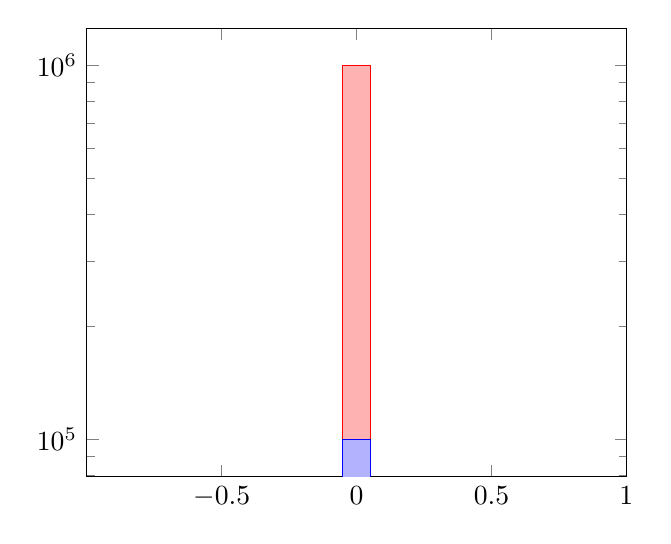
\begin{tikzpicture}
     \begin{axis}[ymode=log
                , ybar stacked
                , log basis y=10
                 ]
          \addplot coordinates {(0,1e5)};
          \addplot coordinates {(0,9e5)};
     \end{axis}
\end{tikzpicture}
\end{minimal}
	The problem is documented as FIXME in pgfplotsstackedpltos.code.tex

	suggested fix: refactor the log and exp methods: always provide the requested basis explicitly, and provide some `prepare log basis' method to improve performance. Do not attach the log basis to the coord math.
\end{bug}

\begin{bug}[prio=1]
	\verb|log number format code| is a global variable and cannot be set for individual axes.

	This applies to \verb|log ticks with fixed point| as well.
\end{bug}

\begin{bug}
	One cannot manually load a table inside of a pgfplots axis if it contains empty lines: the scanline callback is active
\end{bug}

\begin{bug}
	\verb|ybar legend| does not contain \verb|ybar| (sourceforge 3482770)
\end{bug}

\begin{bug}
	\verb|refstyle| does only include partial information of the reference style. (sourceforge 3482770)
\end{bug}

\begin{bug}
	Using square brackets as first char inside of \verb|\legend| leads to a failure: \verb|\legend{[\ion{Ne}{2}],...}|.

	Cause: the \verb|\legend| command does not properly insert \verb|[]| in front of every entry (as it ought to).
\end{bug}

\begin{bug}
	Adding \verb|error bars/.cd| to \verb|\addplot| options causes the \verb|\ref| image to fail. 

	The problem is the key filtering apparently: it discards the \verb|/pgfplots/.cd| but leaves the \verb|error bars/.cd|.
\end{bug}

\begin{bug}
	quiver plots: the clip path does not respect arrow paths
\end{bug}

\begin{bug}[closed]
	
	The default label placement for axis lines=center in 3d appears to be wrong
\begin{verbatim}
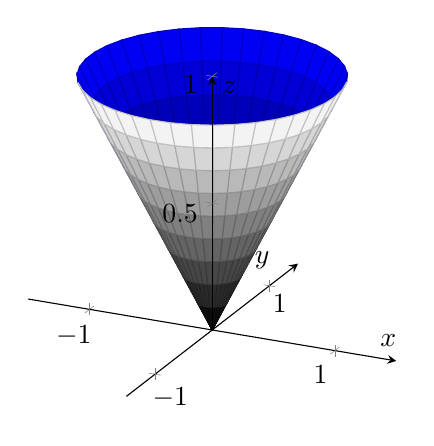
\begin{tikzpicture}
\begin{axis}[
  axis lines=center,
  axis on top,
  xlabel={$x$}, ylabel={$y$}, zlabel={$z$},
  domain=0:1,
  y domain=0:2*pi,
  xmin=-1.5, xmax=1.5,
  ymin=-1.5, ymax=1.5, zmin=0.0,
  mesh/interior colormap=
  	{blueblack}{color=(black) color=(blue)},
  colormap/blackwhite, 
  samples=10,
  samples y=40,
  z buffer=sort,
 ]
  \addplot3[surf] 
  	({x*cos(deg(y))},{x*sin(deg(y))},{x});
\end{axis}
\end{tikzpicture}
\end{verbatim}

	Potential fixes: (a) redefine \verb|right of origin| and its friends for 3d; (b) do not use the \verb|right of origin| things, prefer \verb|rel axis cs=1,0.5,0.5|. Problem: \verb|rel axis cs| must know where the fractions to find the origin (keep in mind that a rel axis value of $0$ means ``lower end''). Perhaps some ``constant'' value should expand to the fraction for zero? 

		Potential fix:
		\url{http://tex.stackexchange.com/questions/84442/pgfplots-labels-and-width-issues-in-non-boxed-3d-plot-with-oblique-projection}
\end{bug}

\begin{bug}
	Alignment bug: axis x line=middle combined with a yshift shifts the xlabel incorrectly:
\begin{minimal}
\documentclass{report}
\usepackage{pgfplots}
\pgfplotsset{compat=1.3}

\begin{document}
  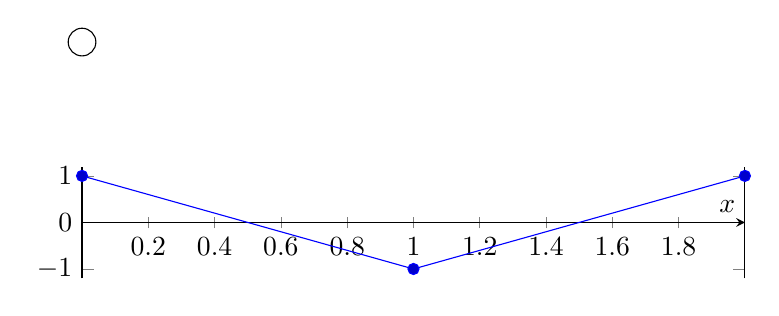
\begin{tikzpicture}
  	\draw (0,0) circle (5pt);
    \begin{scope}[yshift=-3cm]
    \begin{axis}[width=10cm,height=3cm,xlabel={$x$},
        axis x line = middle]
      \addplot coordinates {
        (0,1) (1,-1) (2,1)
      };
    \end{axis}
    \end{scope}
  \end{tikzpicture}
\end{document} 
\end{minimal}
	Using \verb|xlabel style = {yshift=3cm}| in the plot will correctly
position the x label (to its default position). 
\end{bug}

\begin{bug}[closed]
	Using \verb|hide axis| or \verb|axis lines=none| causes the axis to vanish -- but it will still consume space in the bounding box!
	
	A work-around for the user who reported the bug was to use \verb|clip=false|:

\begin{minimal}
\documentclass{article}
\usepackage[utf8]{inputenc}
\usepackage{pgfplots}
\pgfplotsset{compat=1.4}
\begin{document}

\begin{figure}
  \centering
  \fbox{%
  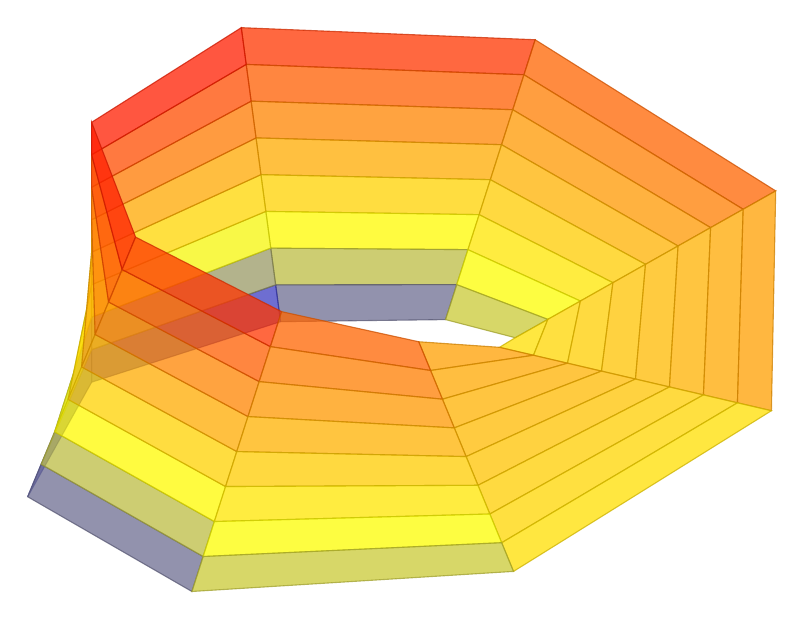
\begin{tikzpicture}
    \begin{axis}[axis equal,scale=2,axis lines=none,clip=false]
      \addplot3[surf,samples=9,domain=-1:1,y domain=0:2*pi,z buffer=sort,opacity=0.75]
         ({cos(deg(y)) * (1 + x/2 * cos(deg(y)/2))},
         {sin(deg(y)) * (1 + x/2 * cos(deg(y)/2))},
         {x/2 * sin(deg(y)/2)});
    \end{axis}
  \end{tikzpicture}}
  \caption{M"obiusband}
\end{figure}

\end{document} 
\end{minimal}

	Interestingly, this does NOT work for 1d plots... here is what I found out today:
	\begin{itemize}
		\item excluding the clip path helps for the example above.
		\item it has no effect for 1d plots (2d axis)
		\item excluding the background path instruction from the low level node causes the bounding box to be empty -- for both 2d and 3d
	\end{itemize}

	See \verb|unittest_hideaxis*|.

	Seems to be better now (with the axis equal scaling fix)
\end{bug}

\begin{bug}[+]
	Adding a decoration to a plot requires \verb|every path/.style={decorate,every path/.style={}}| because pgfplots sets its options inside of a \verb|\scope[<options>]|. 

	This should be fixed.
\end{bug}

\begin{bug}[closed]
	disable tick scale label if the ticks have been disabled.

	\verb|https://sourceforge.net/tracker/index.php?func=detail&aid=3457210&group_id=224188&atid=1060656|
\end{bug}

\begin{bug}[+]
	nodes near coords is broken for layer branch
\end{bug}

\begin{bug}[closed]
	\verb|axis equal,view={0}{90}| for a 3d axis leads to compilation errors (although it seems to work)
\end{bug}

\begin{bug}[closed]
	xbar and nodes near coords does not automatically align the nodes, see \verb|http://tex.stackexchange.com/questions/31701/pgfplots-nodes-near-coords-on-xbar-chart-is-off|
\end{bug}

\begin{bug}[+]
	view direction is imprecise. It seems as if the $z$ direction is wrong.

	See the recent commits on branch \verb|mesh_bg_colormap|
\end{bug}

\begin{bug}
	cannot provide clip path usage in pgfplots commands because of the nested scopes.

	to reproduce, try to give \verb|\addplot+[/tikz/clip]| to some plot.
\end{bug}

\begin{bug}[closed]
	3d: automatic label placement for 'axis lines=center' is buggy
\end{bug}

\begin{bug}
	\verb|\pgfplotsforeachungrouped| cannot be combined with three or more arguments like \verb|\foreach|
\end{bug}

\begin{bug}[+]
	If one specifies \verb|\scope| within an axis, the plots (partially) use their variables, but legends do not.
\begin{minimal}
\documentclass{article}
    \usepackage{pgfplots}
        \pgfplotsset{
            compat=newest,
        }
\begin{document}
    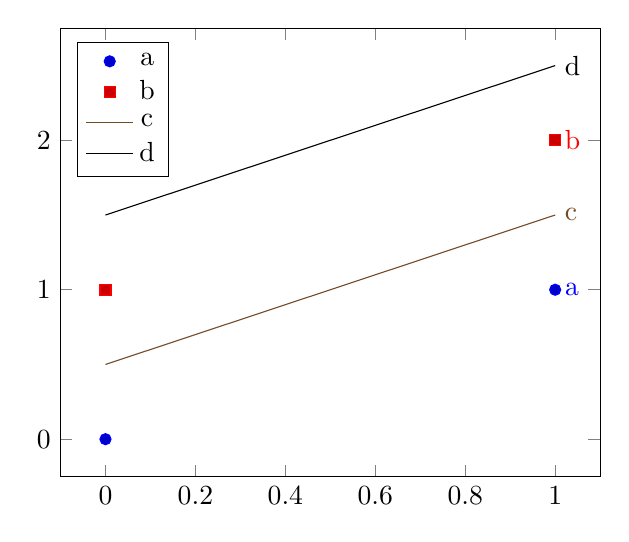
\begin{tikzpicture}
        \begin{axis}[
%                reverse legend,    % uncomment and one entry is missing
                legend pos=north west,
        ]
            \begin{scope}[only marks]
                \addplot
                        coordinates { (0,0) (1,1) } node [right] {a};
                \addplot
%                    [green]        % uncomment and legend does exactly the wrong thing
                        coordinates { (0,1) (1,2) } node [right] {b};
            \end{scope}
            \begin{scope}[mark=none]
                \addplot
                        coordinates { (0,0.5) (1,1.5) } node [right] {c};
                \addplot
%                    [orange]       % uncomment and it works
                                    % (I think this is luck, because it does the same
                                    %  thing as the [green] example above)
                        coordinates { (0,1.5) (1,2.5) } node [right] {d};
            \end{scope}
            \legend{
                a,
                b,
                c,
                d,
            }
        \end{axis}
    \end{tikzpicture}
\end{document}
\end{minimal}
\end{bug}

\begin{bug}
the below example of a latex file gives the following error upon the 2nd run of latex. The first run works fine. This happens both when running dvilualatex and just latex, both from TexLive 2011.

The error:

\begin{verbatim}
...
(/usr/local/texlive/2011/texmf-dist/tex/generic/tex4ht/color.4ht)
(/usr/local/texlive/2011/texmf-dist/tex/generic/tex4ht/html4.4ht)
(/usr/local/texlive/2011/texmf-dist/tex/generic/tex4ht/html4-math.4ht))
(./epub.aux)
! Missing \endcsname inserted.
<to be read again> 
                   \protect 
l.30 \ref{govconsumptionlegend}
                               
?
\end{verbatim}


\begin{verbatim}
\makeatletter

\def\HCode{\futurelet\HCode\HChar}\def\HChar{\ifx"\HCode\def\HCode"##1"{\Link##1}\expandafter\HCode\else\expandafter\Link\fi}\def\Link#1.a.b.c.{\g@addto@macro\@documentclasshook{\RequirePackage[#1,html]{tex4ht}}\let\HCode\documentstyle\def\documentstyle{\let\documentstyle\HCode\expandafter\def\csname tex4ht\endcsname{#1,html}\def\HCode####1{\documentstyle[tex4ht,}\@ifnextchar[{\HCode}{\documentstyle[tex4ht]}}}

\makeatother

\HCode "xhtml,png,charset=utf-8".a.b.c.


\documentclass[11pt,a4paper]{book}

\def\pgfsysdriver{pgfsys-tex4ht.def}
\usepackage{pgfplots}

\pgfplotsset{width=\textwidth,compat=1.3,every axis/.append style={font=\footnotesize},cycle list name=black white}

\begin{document}
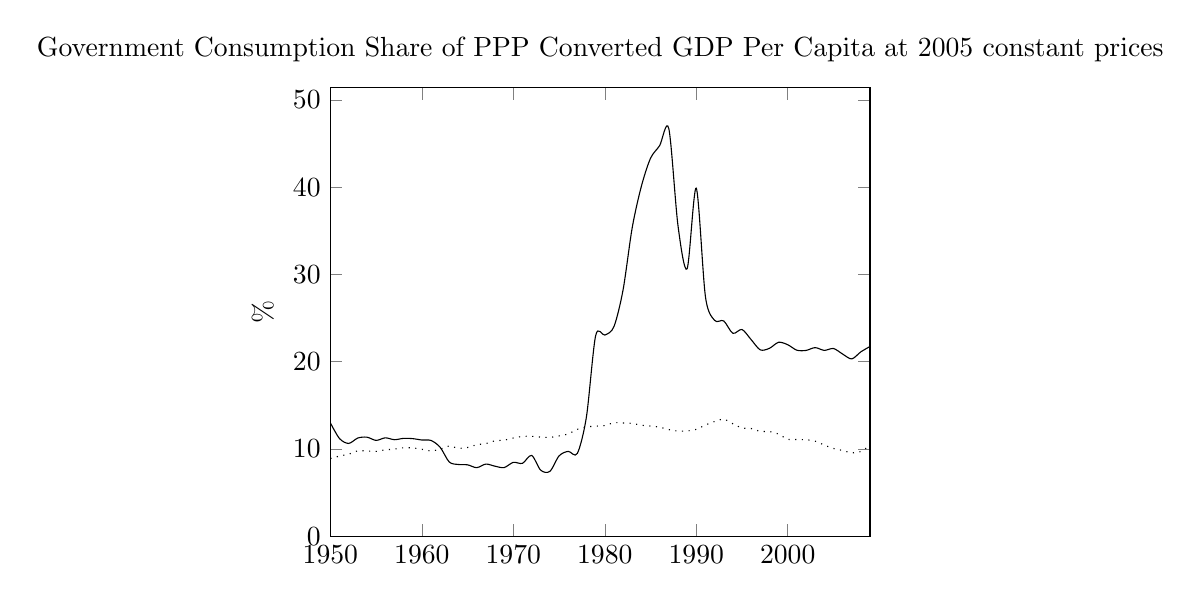
\begin{tikzpicture}

\begin{axis}[ylabel=\%,x tick label style={ /pgf/number format/1000 sep=},ymin=0,xmin=1950,xmax=2009,legend to name=govconsumptionlegend,title=Government Consumption Share of PPP Converted GDP Per Capita at 2005 constant prices] 
\addplot[smooth,solid] coordinates {
(1950,12.98732304) (1951,11.18937899) (1952,10.63447043) (1953,11.25741618) (1954,11.35201741) (1955,10.98310036) (1956,11.27808626) (1957,11.06275337) (1958,11.21626046) (1959,11.18458192) (1960,11.02716074) (1961,10.97486816) (1962,10.19712891) (1963,8.50170024) (1964,8.220444391) (1965,8.181873469) (1966,7.859215042) (1967,8.269806768) (1968,8.023789126) (1969,7.867343418) (1970,8.469691612) (1971,8.352726749) (1972,9.263915297) (1973,7.560088984) (1974,7.436700475) (1975,9.207375031) (1976,9.725811776) (1977,9.495010597) (1978,13.74144043) (1979,22.99348928) (1980,23.05639171) (1981,24.02424559) (1982,28.25010594) (1983,35.38307779) (1984,40.11885923) (1985,43.3304334) (1986,44.7847218) (1987,46.7237337) (1988,35.62924609) (1989,30.65659214) (1990,39.89428582) (1991,27.48910619) (1992,24.75024034) (1993,24.68286164) (1994,23.26013887) (1995,23.69594547) (1996,22.53334681) (1997,21.35901868) (1998,21.53873871) (1999,22.22968487) (2000,21.95238646) (2001,21.3231532) (2002,21.29835897) (2003,21.6183452) (2004,21.30177929) (2005,21.51748623) (2006,20.88675316) (2007,20.32549306) (2008,21.13794484) (2009,21.75075984) 
};
\addlegendentry{Country 1}
\addplot[smooth,dotted] coordinates {
(1950,8.90574995) (1951,9.181850378) (1952,9.4040808) (1953,9.790597533) (1954,9.766571438) (1955,9.721345475) (1956,9.898347958) (1957,9.986947451) (1958,10.13725015) (1959,10.11995062) (1960,9.9669931) (1961,9.781482565) (1962,9.968596797) (1963,10.33417822) (1964,10.07453069) (1965,10.17668623) (1966,10.4859246) (1967,10.6188237) (1968,10.93369976) (1969,11.01396095) (1970,11.25808879) (1971,11.43128231) (1972,11.45138898) (1973,11.36045323) (1974,11.33276575) (1975,11.50069671) (1976,11.72466305) (1977,12.25394557) (1978,12.52158998) (1979,12.61603185) (1980,12.68712893) (1981,13.01282874) (1982,12.97669774) (1983,12.92432378) (1984,12.72145426) (1985,12.63447969) (1986,12.49591698) (1987,12.22704263) (1988,12.05291461) (1989,12.07675903) (1990,12.25254614) (1991,12.74485006) (1992,13.14305947) (1993,13.41082617) (1994,12.89670369) (1995,12.41585298) (1996,12.34588672) (1997,12.01926401) (1998,12.00221677) (1999,11.69852271) (2000,11.11468531) (2001,11.08248726) (2002,11.05693806) (2003,10.89817902) (2004,10.44900187) (2005,10.05582475) (2006,9.829361577) (2007,9.567882534) (2008,9.714898563) (2009,10.42225882)
};
\addlegendentry{Country 2}
\end{axis}\end{tikzpicture}

\ref{govconsumptionlegend}

\end{document}
\end{verbatim}
\end{bug}

\begin{bug}[+]
	the table package does not support non-ASCII column names. If there are non-ASCII column names, it might fail to produce a readable error message.
\end{bug}

\begin{bug}[prio=2]
	 \#3213889 hyperref boxes are in wrong position for vertical labels

	see \url{http://tex.stackexchange.com/questions/13364/how-to-make-pgfplots-vertical-labels-have-proper-hyperref-erence-box
} for problem description and potential fixes

\end{bug}

\begin{bug}[prio=1]
CRASH:
\begin{minimal}
\begin{tikzpicture}
	\begin{axis}[
		scale mode=scale uniformly,
		x={(1pt,0pt)},
		y={(-0.5pt,0.5pt)},
		z={(0pt,1pt)},
	]

	% addplot3 works (with 3d coords):
	\addplot coordinates {
		(0,0) (1,0) (0,1)
	};
		
	\end{axis}
\end{tikzpicture}
\end{minimal}
\end{bug}

\begin{bug}[prio=1]
	Using $0$ in pgfplots coordinate systems does not necessarily mean ``no offset''. This is misleading. Bug sourceforge \#3168030:
\begin{minimal}
\documentclass[a4paper]{article}
\usepackage{german}
\usepackage[utf8]{inputenc}

\usepackage{pgfplots}

\usepackage{pgfplotstable}
\usepackage{booktabs}
\usepackage{array}
\usepackage{colortbl}

\begin{document}

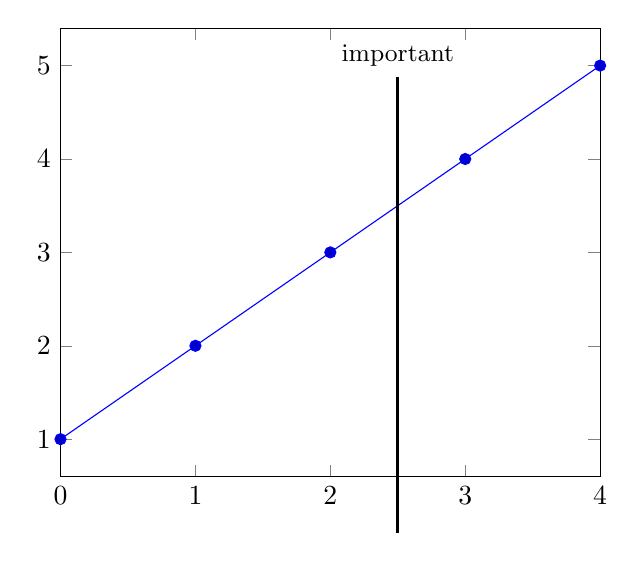
\begin{tikzpicture}
	\begin{axis}[enlarge x limits=false, extra description/.code={\draw[very thick] (axis cs:2.5,0) -- ++(rel axis cs:0,1.1) node[above,align=center,font=\small]{important};}								]
		\addplot coordinates{
							(0,1)
							(1,2)
							(2,3)
							(3,4)
							(4,5)};
	\end{axis}
\end{tikzpicture}

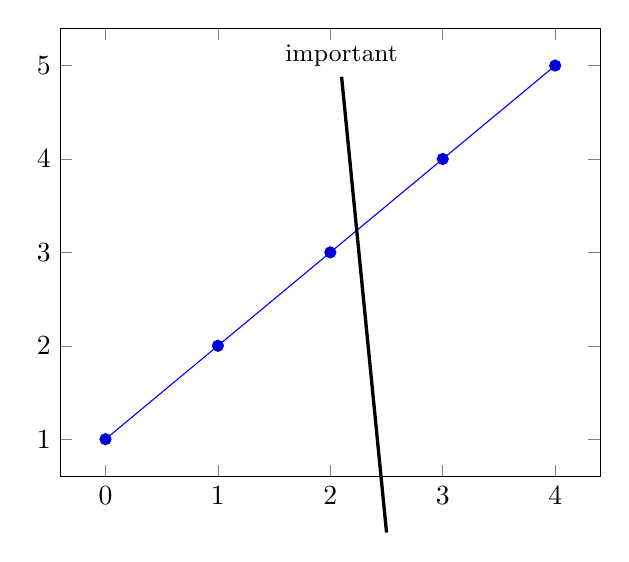
\begin{tikzpicture}
	\begin{axis}[enlarge x limits=true,	extra description/.code={\draw[very thick] (axis cs:2.5,0) -- ++(rel axis cs:0,1.1) node[above,align=center,font=\small]{important};}								]
		\addplot coordinates{
							(0,1)
							(1,2)
							(2,3)
							(3,4)
							(4,5)};
	\end{axis}
\end{tikzpicture}
\end{document}


\end{document}

\end{minimal}
\end{bug}


\begin{bug}[prio=2]
	The clipping of tick lines uses the middle of axis lines; it does not incorporate the line width of the axis lines.
\begin{minimal}
\documentclass{article}
\usepackage{pgfplots}
\pgfplotsset{compat=1.3,
              every axis/.append style={semithick},
              every tick/.append style={semithick,color=black},
              tick align=outside
             }
\begin{document}
   \thispagestyle{empty}
   \begin{figure}[p]
     \centering
     \begin{tikzpicture}
       \begin{axis}[xmin=0,
                    xmax=30,
                    ymin=0,
                    ymax=1.2
                   ]
       \end{axis}
     \end{tikzpicture}
   \end{figure}
\end{document}

\end{minimal}
\end{bug}

\begin{bug}[prio=2]
can someone confirm the following behavior. The y label of a plot gets
truncated in some circumstances if the external library is used. This
happens for me if no title is specified for a plot. Consider the
following example:

\begin{minimal}
\documentclass[11pt,a4paper]{article}

\usepackage{tikz}
\usepackage{pgfplots}

\pgfplotsset{compat=1.3}
\usepgfplotslibrary{external}
\tikzexternalize[force remake]

\begin{document}
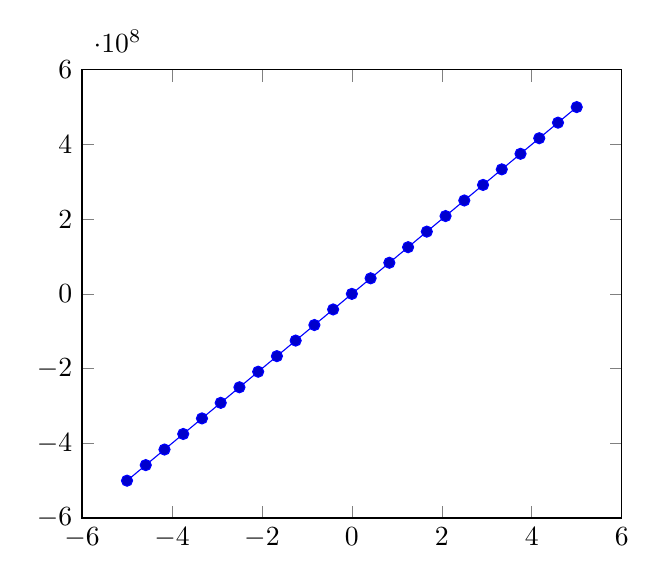
\begin{tikzpicture}
\begin{axis}[y tick scale label style={inner sep=1pt}]
\addplot {x * 10^8};
\end{axis}
\end{tikzpicture}
\end{document}

\end{minimal}
\end{bug}


\begin{bug}[prio=8,+]
	Decorations in plots appear to be problematic (this is a duplicate! caused by the fact that decorate=false is used at the beginning of every plot, need to adjust every path style):
\begin{minimal}
\documentclass{scrartcl}

\usepackage{pgfplots}
\usetikzlibrary{decorations}

\begin{document}
\begin{tikzpicture}

\begin{axis}

\addplot+[postaction={draw, decorate, decoration=border}] coordinates {(0,0) (5,0.5)}; %funktioniert nicht

\end{axis}

\draw [postaction={draw, decorate, decoration=border}] (0,-3cm)  -- ++(5cm,0.5cm); %funktioniert 

\end{tikzpicture}

\begin{tikzpicture}

\begin{axis}

\addplot+[postaction={draw, decorate, decoration=border},
        % tedious, but necessary: pgfplots accidentally resets the
        % "decorate" option at the beginning of the path (probably a
        % bug).
        % This is a work-around:
        every path/.style={
            postaction={decorate},
            every path/.style={},
        }, 
	] coordinates {(0,0) (5,0.5)}; %funktioniert nicht

\end{axis}

\end{tikzpicture}
\end{document}
\end{minimal}

\end{bug}

\begin{bug}[prio=10,closed]
	Markers in legends are not (always?) filled properly
\begin{minimal}
\documentclass{article}
    \usepackage{pgfplots}
    \usepackage{pgfplotstable}
\begin{document}

    \begin{tikzpicture}
        \begin{axis}
            \addplot [mark=*,only marks] coordinates { (-1,1) (1,-1) };
            \legend{measured data}
        \end{axis}
    \end{tikzpicture}
\end{document}
\end{minimal}
	caused by the fact that options of `every axis legend' are in effect at this time -- which includes \verb|fill=white|.
\end{bug}

\begin{bug}[prio=11,closed]
	polar lib: the clipping of markers doesn't work correctly for partial polar axes.
\end{bug}

\begin{bug}[prio=1]
	The legend has the \verb|text depth=0.15em| initial configuration, which is extremely bad for legend entries with huge depth (large fractionals or formulas?)
\end{bug}

\begin{bug}
	\url{http://groups.google.at/group/comp.text.tex/msg/adcb1d071c2cba40}

	If I use a yshift in a scope to draw two graphs superimposed, the x
label in the second plot (the one in the yshift scope) is not
positioned correctly. I need to manually add another yshift, with the
same value in the opposite direction, to get the label at the correct
place. This happens if the \verb|axis x line = middle| option is used.
Without that option, the x label is positioned correctly. Example
follows: 
\begin{minimal}
\documentclass{article}

\usepackage{pgfplots}

\pgfplotsset{compat=1.3}

\begin{document}

  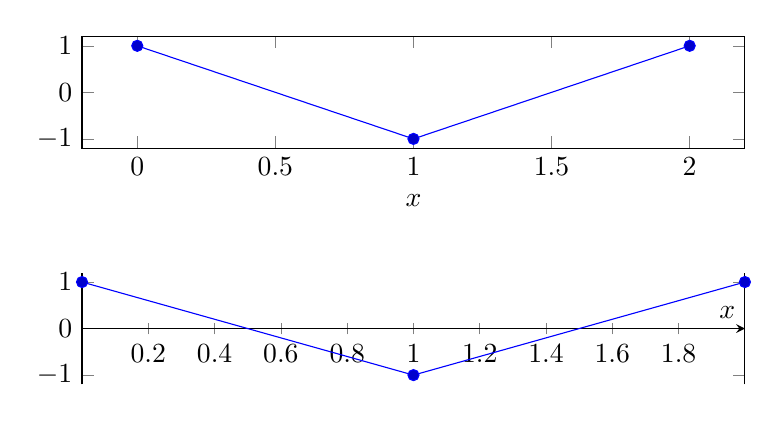
\begin{tikzpicture}
    \begin{axis}[width=10cm,height=3cm,xlabel={$x$}]
      \addplot coordinates {
        (0,1) (1,-1) (2,1)
      };
    \end{axis}
    \begin{scope}[yshift=-3cm]
    \begin{axis}[width=10cm,height=3cm,xlabel={$x$},
        axis x line = middle]
      \addplot coordinates {
        (0,1) (1,-1) (2,1)
      };
    \end{axis}
    \end{scope}
  \end{tikzpicture}
\end{document}
\end{minimal}

Using \verb|xlabel style = {yshift=3cm}| in the second plot will correctly
position the x label (to its default position).

Gab
\end{bug}

\begin{bug}[prio=2,closed]
	One cannot load the clickable lib before pgfplots:
see also \url{https://sourceforge.net/tracker/?func=detail&atid=1060656&aid=3033981&group_id=224188}
\end{bug}

\begin{bug}[closed]
	the unit vector ratio impl does not work as intended: the manual example
\begin{minimal}
\documentclass{article}

\usepackage{pgfplots}
\begin{document}
\begin{tikzpicture}
\begin{axis}[axis equal]
% FokkerDrI_layer_0.patches.dat contains:
% # each row is one vertex; three consecutive 
% # vertices make one triangle (patch)
% 105.577	-19.7332	2.85249	
% 88.9233	-21.1254	13.0359	
% 89.2104	-22.1547	1.46467	
% # end of facet 0
% 105.577	-19.7332	2.85249	
% 105.577	-17.2161	12.146	
% 88.9233	-21.1254	13.0359	
% # end of facet 1
\addplot3[patch] 
	file
	{plotdata/FokkerDrI_layer_0.patches.dat};
\end{axis}
\end{tikzpicture}
\end{document}
\end{minimal}
	fails and resorts to guesses!
\end{bug}

\begin{bug}[prio=3]
	\verb|\addplot table[blue]| ignores the color options!
\end{bug}

\begin{bug}[prio=1,+]
	providing \verb|ymin=0| for a logarithmic axes has no effect; and there is no sanity checking	
\end{bug}

\begin{bug}[prio=1]
	The \verb|mark list| produces a lot of

\begin{verbatim}
\XC@edef #1#2->\begingroup \ifnum \catcode `\!=13 \edef !{\string !}\fi \ifnum \catcode `\:=13 \edef :{\string :}\fi \ifnum \catcode `\-=13 \edef -{\string -}\fi \ifnum \catcode `\+=13 \edef +{\string +}\fi \ifnum \catcode `\;=13 \edef ;{\string ;}\fi \ifnum \catcode `\"=13 \edef "{\string "}\fi \ifnum \catcode `\>=13 \edef >{\string >}\fi \edef #1{#2}\@onelevel@sanitize #1\aftergroupdef #1#1
[........]
{\if}

\@@tmp ->.!80!black
{true}
{the character !}
Missing character: There is no ! in font nullfont!
{the character 8}
Missing character: There is no 8 in font nullfont!
{the character 0}
Missing character: There is no 0 in font nullfont!
{the character !}
Missing character: There is no ! in font nullfont!
{the character b}
Missing character: There is no b in font nullfont!
{the character l}
Missing character: There is no l in font nullfont!
{the character a}
Missing character: There is no a in font nullfont!
{the character c}
Missing character: There is no c in font nullfont!
{the character k}
Missing character: There is no k in font nullfont!
{\def}
{\else}
\end{verbatim}
	bugs. Probably fixed with more recent version of xcolor?
\end{bug}

\begin{bug}[closed]
	It is not possible to provide \verb|#| comments in inline tables.
\begin{verbatim}
\pgfplotstabletypeset[
]{
# GHz dB
1 0
2 -10
3 0
}
\end{verbatim}
	The problem occurs since the \verb|#| has special handling and many internal checks fail. I started to implement special handling, but that might require vast changes.

	One solution is to use
\begin{verbatim}
\toks0={#1}
\edef\macro{\the\toks0}
\end{verbatim}
	instead of 
\begin{verbatim}
\def\macro{#1}
\end{verbatim}
	anywhere in the code -- the \verb|\def| introduces special checks for the \verb|#| whereas the \verb|\toks| does not.
\end{bug}

\begin{bug}[prio=7,+]
	It is not possible to use \verb|\addplot ... node[pos=0.5] {a};| in pgfplots.

	Reason: the timer information is tikz high level, but pgfplots uses the PGF basic layer.

	DONE.

	Open: the \verb|\pgfplotspointplotattime| should provide more useful output: SCI notation and it should respect custom trafos
\end{bug}


\begin{bug}[closed]
	Groupplots + named nodes doesn't yield the correct output. Perhaps scoping difficulties? Or problems adjusting the stored coords?
\begin{minimal}
\documentclass[10pt]{article}

\usepackage{pgfplots}
\usepgfplotslibrary{groupplots}

\begin{document}

\begin{tikzpicture}%
%\begin{axis}[%
\begin{groupplot}[%
	group style={group size=1 by 1},%
]%
	\nextgroupplot;
	\node[name=a] at (axis cs:0.1,-1) {N};
	\addplot coordinates{(0,1) (1,2)};
\end{groupplot}
%\end{axis}

\draw (a) circle (5pt);
\end{tikzpicture}%
\end{document}
\end{minimal}
\end{bug}

\begin{bug}[prio=1]
	providing \verb|\legend{}| without any \verb|\addplot| commands causes a problem
\end{bug}

\begin{bug}[prio=3,closed]
	It is not (properly) possible to provide \verb|surf| to \verb|\addplot|.
\begin{verbatim}
\begin{tikzpicture}
\begin{axis}[]
	\addplot[surf,domain=0:720,samples y=25] {cos(x)*sin(y)};%
\end{axis}
\end{tikzpicture}
! Package pgfplots Error: Sorry, you can't use 'y' in this context. PGFPlots expected to sample a line, not a mesh. Please use the [mesh] option combined with [samples y>0] and [domain y!=0:0] to indicate a twodimensional input domain.
\end{verbatim}

	OK, I've been working on it:
	\begin{itemize}
		\item it is now possible to use \verb|\addplot[surf]| and it works.
		\item it is \emph{not} yet possible to \emph{sample} matrices with \verb|\addplot[surf]|.

			I added the \verb|sample dim| key. But it does not work yet... the plot expression implementation needs to be refactored.
	\end{itemize}
\end{bug}

\begin{bug}[closed]
	Verify that the list termination (either with \verb|\\| or with \verb|,|) works correctly
\end{bug}

\begin{bug}[closed]
	ternary lib: \verb|\addplot| doesn't work correctly, only \verb|\addplot3|
\end{bug}

\begin{bug}[open]
	after using a preset key (milli) with x SI prefix, Next, I want to switch to the normal mode, so I write simply: x SI prefix=none, unfortunately the 'none' value is undefined and the compilation can not proceed
\end{bug}

\begin{bug}[closed]
I'm trying to create an extra y tick on a plot, but I want the tick and 
label to be on the right side of the plot. I want all the other y ticks 
and labels are all on the left side of the plot.

It's almost working properly, but it won't put the extra label on the 
right side of the plot where I want it.  The tick is appearing on the 
right side, but the label is staying on the left side with all the other 
labels. I was using version 1.2.2 before and this was working fine, but 
I just upgraded to version 1.4 because I wanted to use a new feature 
that wasn't present in 1.2.2.  Is it possible this was broken somewhere 
along the way?

\begin{minimal}
\documentclass{article}
\usepackage{pgfplots}
\begin{document}
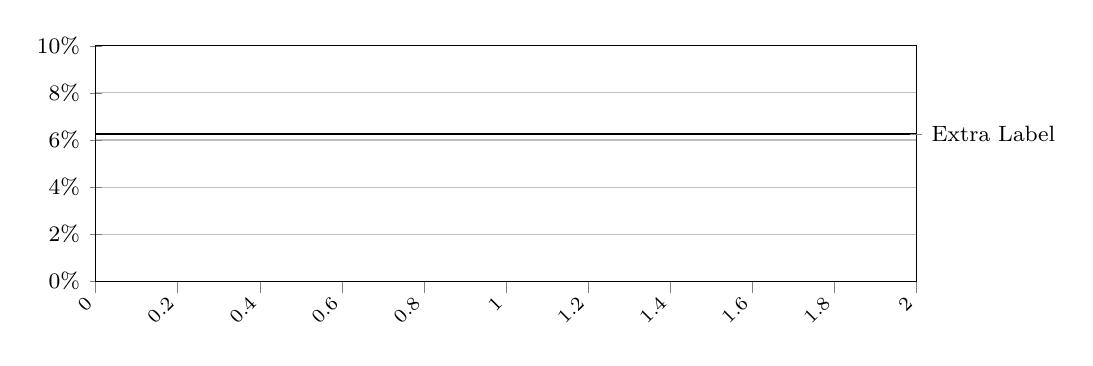
\begin{tikzpicture}
\begin{axis}[
         small,
         width=12cm,
         height=1.8in,
         ymin=0,
		 ymax=10,
         xmin=0,
		 xmax=2,
         ybar,
         ymajorgrids=true,
         yminorgrids=false,
         minor y tick num=0,
         ytick pos=left,
         xtick pos=left,
         ytick align=center,
         yticklabel={$\pgfmathprintnumber{\tick}\%$},
         xtick align=outside,
         x tick style={},
         xticklabel style={rotate=45,anchor=east,font=\scriptsize\sffamily},
         extra y tick style={tick pos=right, ticklabel pos=right, grid 
style={thick,color=black}},
         extra y ticks={6.25},
         extra y tick labels={Extra Label},
]

%\addplot plot[error bars/.cd,y dir=plus,y explicit,x dir=none] table 
%[x=Index,y expr=100*\thisrow{AvgLocked},y error=Diff]{locked_tabbed.dat};

\end{axis}
\end{tikzpicture}
\end{document}
\end{minimal}
\end{bug}

\begin{bug}[-,prio=1]
 the axis line combination styles can't be adjusted for 3D because they are
  evaluated too early.
\end{bug}

\begin{bug}[-,closed]
  external lib + dvi/ps + windows: it seems the ';' doesn't work; use '\&' to
  separate commands
\end{bug}

\begin{bug}[-]
  check y tick scale label for 2nd y axis
\end{bug}

\begin{bug}[closed]
  foreach variants in pgfplots accept only one parameter
\begin{verbatim}
%            \foreach \x/\y in {1/a, 2/b, 3/c}
%                {\node at (axis cs:0,\x) {\y};}%   % doesn't work
%            \pgfplotsforeachungrouped \x/\y in {1/a, 2/b, 3/c}
%                {\node at (axis cs:0,\x) {\y};}%   % doesn't work
\end{verbatim}
\end{bug}




\begin{bug}[-]
  groupplots + extra braces or foreach are incompatible.
\end{bug}

\begin{bug}[-]
  numplotspertype and forget plot and ybar interval yields errors.
\end{bug}

\begin{bug}[-]
  expression plotting and empty 'y' results in errors. Perhaps it would be
  better to handle that explicitly somehow?
  (occurs for hist when one input line is empty)
\end{bug}

\begin{bug}[-,closed]
  view normal vector does not correctly respect plot box ratio and x dir
\end{bug}

\begin{bug}[closed]
  plot box ratio  has a strange input format (compare with unit vector ratio).
\end{bug}

\begin{bug}[-,closed]
  clickable and Windows Acrobat Reader 9 has been reported to fail

  it this still active?
\end{bug}

\begin{bug}[-]
  /pgfplots/samples at and /tikz/samples at work on the same axe. Tantau says that this key support foreach statement and thus the dotes notation. However, when I want to use two or more different dots notation within pgfplots, latex crashes !
Here is an example which clarify this issue :
\verb|\addplot+[mark=none,variable={\t}, samples at = {\foreach \x in {0,10,...,180,200,...340} {\x, }360}] ({sin(t*2)}, {cos(t)}); |
\end{bug}

\begin{bug}[-,prio=2]
  potential incompatibility: clickable and external. The clickable lib writes
  into pgfplots.djs which might cause multithreaded problems.
\end{bug}

\begin{bug}[-]
  groupplots: mixing 2d/3d in one groupplot doesn't reset 'zmin,zmax' ?
 
\end{bug}

\begin{bug}[+]
  'clip=false' does not disable marker clipping!
\end{bug}


\begin{bug}[closed]
  multiple ordinates: grid lines are drawn on top of function plots; that's bad.
Check: 
 I think you have to change the process line previousely invoked, and make the axes generation at the end :
1. generating adequate grid $\leadsto$ 2. plotting functions $\leadsto$ 3. creating axes, tick nodes...
You can take a minute look at figure 1 @ "The addplot Command: Coordinate Input" section 4.2 p 19.
and you can remark that colour filling overlaps x- and y-axis ! So I suggest that you use "excute at end picture=<axis generation code>" tikz option or similar to avoid this issue.


	$\to $ Should be fixed with layers
\end{bug}

\begin{bug}[-]
  3D axes: it is difficult to get an 1:1 correspondence to tikz.
\end{bug}

\begin{bug}[closed]
  3D axes: providing three unit vectors is not sufficient, one also needs to set
  'view={}{}'. That should be done automatically.
  
- 3D axes: Providing three unit vectors manually yields incorrect axis
  initialisation.
\end{bug}

\begin{bug}[-]
  3D axis: provide support for manual axis configuration, 
  	- depth (n vector),
	- foreground/background,
	- tick label axes,
	- ...
\end{bug}

\begin{bug}[closed]
	WONTFIX.

  Patch plots: directly transform cdata. Should simplify interpolation during
  refine/triangulation etc. and shouldn't make a difference otherwise.
\end{bug}

\begin{bug}[closed]
  manual errors of given pgfplots\_unstable version:
 94	2.5.12	\verb|addplot+[patch] --> addplot3+[patch]|
162 			"xmode, ymode, zmode" and "x dir, ..." 
			come again on page 177
\end{bug}

\begin{bug}[closed]
  don't loose \verb|\ref|'s when externalizing
  I'll provide a minimal later
\end{bug}


\begin{bug}[-,closed]
  incompatibility pdfpages (most recent version), MikTeX and tikz external lib
  (something with shipout routine)
\end{bug}

\begin{bug}[-]
  plot graphics: \verb|\ref| legend doesn't work properly
\end{bug}

\begin{bug}[+,prio=9]
  french babel and colorbars are not fully compatible. The problem is that
  colorbars use '\verb|\addplot| graphics {};' with a fixed catcode for the ';' --
  which might lead to problems.
\end{bug}

\begin{bug}[closed]
  markers should not be drawn on top of everything else. Always restore the
  clipping region for each plot.
 
\end{bug}

\begin{bug}[-,closed]
  mesh/patch plots:
  	- jump thing + z buffer=sort probably doesn't work
\end{bug}

\begin{bug}[-]
  ternary axes: the 'marker clipping' doesn't work (naturally)
\end{bug}

\begin{bug}[-]
  polar axes: 
  \begin{itemize}
	\item \ok is wrong since 'near ticklabel' anchor uses pointunitx which is not correctly initialised for polar axes.
	\item  axis equal
	\item \ok data scaling needs to be disabled for X axis.
	\item \ok auto tick labels work only for the case of disabledatascaling
\end{itemize}
\end{bug}

\begin{bug}[-]
  contour:
  	the table/meta=2  default is wrong.
\end{bug}

\begin{bug}[-,prio=2]
  OK    : 'every node near coord/.append style={scale=0.7}'
  NOT OK: 'every node near coord/.append style={scale=0.7},ybar'
  -$\leadsto$ sequence of shift and scale matters ...
\end{bug}



\begin{bug}[-]
  dimension too large sanity checking: TeX uses the maximum value instead.
  Perhaps that can be checked?
\end{bug}

\begin{bug}[-,prio=2]
  view={0}{90}  and enlargelimits=auto is not always satisfactory: it disables enlarged
  limits, but for contours, I'd like to have it.
  What is to do?
\end{bug}

\begin{bug}[-,closed]
  provide remark at end document "Package pgfplots: consider using the preamble
  command \verb|\pgfplotsset{compat=1.3} to improve label placement|"
\end{bug}

\begin{bug}[-,prio=1]
  there are a lot of .code 2 args styles which do not support spaces between
  their arguments. Fix this.
\end{bug}

\begin{bug}[-,closed]
  contour external should allow different variations how to deal with
  end-of-scanline markers. gnuplot requires empty lines; matlab doesn't deal
  with them as far as I know.
\end{bug}

\begin{bug}[-,prio=2]
  contour external doesn't handle explicitly provided matrix data (mesh/rows and
  mesh/cols) yet.
\end{bug}

\begin{bug}[-,prio=2]
  contour external doesn't handle the ordering flag correctly.
\end{bug}

\begin{bug}[-]
  the quiver/scale arrows   thing might need an "auto" option. If I don't add it
  now, it'll probably never work in the future.
\end{bug}

\begin{bug}[-]
  `1.23456e4;'  in a log plot resulted in hard-to-read error messages. Improve
  sanity checking here.
\end{bug}

\begin{bug}[-,prio=2]
  the title style for 'footnotesize' is not as I want it to: it doesn't respect
  the depth below the baseline. Or does it need a \verb|\strut|?
\end{bug}

\begin{bug}[-,epic=Usability]
  avoid dimension too large errors which occur due to a data range restrictions.
  Example:
  data range = 0:6000
  view range = 0:1
  $\leadsto$ results in error.
  But that's easy to detect! Just compute the point coordinate in float (after
  the scaling is complete). Then, install a filter somewhere. perhaps an "a
  posteriori" filter in the pointxyz command?

	DUPLICATE:
	the nasty dimension-to-large message could probably be avoided if pgfplots would simply clip the results to TeX's range
\end{bug}


\begin{bug}[-,closed]
  the autodetection of the '\verb|\\|' list format is buggy: it should return true if
  and only if the last element is '\verb|\\|', not if '\verb|\\|' occurs inside of the
  argument.
\end{bug}


\begin{bug}[-]
  \verb|yticklabels={<list>}, extra y ticks={...}|  is incompatible since the extra
  ticks share the same tick typesetting routine (which, in turn, queries the
  <list>). 
\end{bug}

\begin{bug}[-,closed]
  '\verb|\addplot[only marks]|' does not assign a plot mark; one needs 'mark=*'
  explicitly. that's confusing...

  see also \url{https://sourceforge.net/tracker/?func=detail&atid=1060656&aid=3045389&group_id=224188}
\end{bug}

\begin{bug}[-]
  The 'text depth' in legend entries is incompatible with 'text width'.
  The problem: text width is implemented using \verb|\begin{minipage}[t]|
  so its contents is all in the depth. Setting text depths overrides the
  height!
\end{bug}

\begin{bug}[-,prio=1]
  the '/pgfplots/table/.search also' is overwritten during \verb|\addplot table| with
  /.search also={/pgfplots}. That's not so good.
\end{bug}

\begin{bug}[-]
  one can't provide 'disable log filter' to addplot (but it might be
  interesting)
\end{bug}

\begin{bug}[-]
  FPU: atan doesn't check for unbounded inputs.
\end{bug}

\begin{bug}[-]
  unbounded inputs: improve warning messages: they should not contain low level
  FPU args.
\end{bug}

\begin{bug}[-]
  the user interface to set 'tickwidth=0' for a SINGLE axis is not very good: it seems one needs 'xtick style={/pgfplots/tickwidth=0}' to do so...
	$\leadsto$ can be solved if tickwidth has a family, I guess. Something like 'draw' which will not be pulled by pgfplots. But then remains a problem of key paths.
	
\end{bug}

\begin{bug}[-]
  I have seen that 'plot table' with very large files can produce pool size problems -- even if the coordinates are all filtered away.
	In other words: the code can't simply read a file and throw its contents away.
	The problem appears to be some math parsing using the table/x expr and friends.
	'pool size = names of control sequences and file name'
	$\leadsto$ the math parser could be improved with ifcsname
\end{bug}

\begin{bug}[-,closed]
  axis lines and 3D: some tick lines are not drawn, see manual examples
\end{bug}

\begin{bug}[-,closed]
  check for placement of tick scale label for compat=newest
	$\leadsto$ I improved them for 2d and 3d
	$\leadsto$ needs some further checks, I guess
	
\end{bug}

\begin{bug}[-]
  providing zmin/xmax to an axis activates 3D mode, ok -- but lower dimensional input routines appear to fail.
\end{bug}

\begin{bug}[-]
  one can't provide 'scale' as argument to a (3d) axis
\end{bug}

\begin{bug}[closed]
  getthisrow still has to be fixed
\end{bug}

\begin{bug}[-]
  it may still happen that log-axes get only *one* tick label (in my case \verb|10^{-0.2}|). That should never happen.
	The range is about ymin=4.7e-1, ymax=9.5e-1
\end{bug}

\begin{bug}[-]
  log samples in plot expression for 3D plots
\end{bug}

\begin{bug}[-]
  different log bases and gnuplot
\end{bug}

\begin{bug}[+]
  3D gnuplot: z buffer fails (see tests)
\end{bug}

\begin{bug}[-]
  I tried placing a named coordinate inside one axis and using it in
	another. It failed.

	 CF: The axis is drawn inside of its own picture which will only be shifted if everything has been drawn. That will be the origin of this problem I guess

	Miraculously I can use the coordinate outside axis env. So I have
	reached the following solution:
\end{bug}

\begin{bug}[-]
  plot coordinates doesn't check too well if 
	1. addplot3 is used but only two coords are given
	2. addplot is given but three coordinates are provided (also for plot expression)
\end{bug}

\begin{bug}[+]
  gnuplot: set terminal table seems to be deprecated.
\end{bug}

\begin{bug}[closed]
  gnuplot and 3D
	$\leadsto$ I need a shared interface to prepare the required keys for expression plotting
\end{bug}

\begin{bug}[-]
  the compat things are not yet complete: I wanted to check when it is really necessary (for example if 'x dir' is used)
\end{bug}

\begin{bug}[-]
  the nodes near coords feature produces unexpected results when used together
  with markers $\leadsto$ this is due to the default configuration of scatter plots.
\end{bug}


\begin{bug}[closed]
  check whether /pgfplots/ keys are processed properly in legends. This is
  certainly not the case for the \verb|\label/\ref| legend!
  $\leadsto$ which ones are the problem?
\end{bug}

\begin{bug}[-]
  the ybar style won't be set inside of \verb|\label{}|
\end{bug}


\begin{bug}[-]
  axis equal for semilog plots is not correct (?)
\end{bug}



\begin{bug}[-]
  backwards compatibility problem:
  	axis descriptions can't contain /pgfplots/ styles any longer! This is a key
	path issue :-(
\end{bug}


\begin{bug}[-]
  BUG: in empty axes, '\verb|xtick=\empty|' is ignored.
\end{bug}

\begin{bug}[closed]
  finish impl of ticklabel pos.
  I should use the same thing for tickpos as well.
  And: the default arg processing which uses ticklabel pos = tickpos needs to be
  fixed.
  the 2D axes are wrong.
\end{bug}


\begin{bug}[-]
  The automatic tick labeling sometimes produces inconsistent or confusing
  labels:
  	1. engineering and fixed number style are mixed up. 
	2. If range of an axis is so small that the labels differ only on the third
	   decimal, still only two decimals are used. 
\end{bug}


\begin{bug}[closed]
  3D: axis equal implementation might not be correct (at least not for view
  special cases)
\end{bug}

\begin{bug}[-]
  3D:
  	error bars and 
	stacked plots
	need to be updated.

	Is this still current? There has been a major revision some time ago...
\end{bug}

\begin{bug}[closed]
  the \verb|\thisrow| commands in the table package does not (always) respect aliases!
\end{bug}

\begin{bug}[-,prio=2]
  interp shader is displayed transparently in evince

  Bug in evince (for sure). What is to be done?
\end{bug}

\begin{bug}[-]
\begin{verbatim}
  3D:  the use of \addplot3 and \addplot is not sanitized properly
	Possibilities:
	-  used \addplot  when \addplot3 should have been used
	-  used \addplot3 where \addplot should have been used.
	 What can happen here!? Shouldn't this work in every case?
 
- The "xtick" value is not applied unless there is a coordinate in the x range:
	$\leadsto$ that's the handling of empty figures...
	not working:
	  \begin{axis}[xtick=0]
	  \end{axis}
	not working:
	  \begin{axis}[xmin=-5,xmax=5,xtick=0]
	  \end{axis}
	not working:
	  \begin{axis}[xmin=-5,xmax=5,xtick=0]
		\addplot coordinates { (-10, 0) };
	  \end{axis}
	working:
	  \begin{axis}[xmin=-5,xmax=5,xtick=0]
		\addplot coordinates { (0, 0) };
	  \end{axis}
\end{verbatim}
\end{bug}

\begin{bug}[-,closed]
  think about basic level commands for the axis lines -- this should also allow
  \verb|\pgfpathclose| !
\end{bug}


\begin{bug}[closed]
  the arguments to \verb|plot file[#1] and plot table[#1]| are not consistent with
  rest. They need to be treated as behavior options (maybe in a different key
  path).
\end{bug}


\begin{bug}[closed]
  verify that 'draw=none' works! Is something broken here?
	$\leadsto$ write tests!
	+ it appears to be desired that (at least some) markers invoke
	  \verb|\pgfusepathqfillstroke|
	  $\leadsto$ they always 'draw', regardless of tikz color settings.
	  $\leadsto$ ok, I patched that in my marker code... (hackery :-( )
	- no, it works only partially:
	  	draw=none or fill=none works as expected.
		But 'blue' disables filling!?
	- Possible fix:
	  	Overwrite \verb|\filltrue \fillfalse, \drawtrue, \drawfalse|:
			they should set a further boolean '\verb|\drawbooleanhasbeenset|' and
			'\verb|\fillbooleanhasbeenset|'.
		$\leadsto$ Replace the \verb|\pgfusepathqfillstroke| if and only if the respective
		booleans have been set *explicitly*. If they are unchanged, fall back to
		a "reasonable" default.
	  
\end{bug}

\begin{bug}[-,prio=1]
  In 3D case axis [xyz] line != box, there is just ONE hyperplane.
  My implementation works only if either ALL are box or ALL are 'middle'.
\end{bug}

\begin{bug}[closed]
  3D case : grid lines work correctly, but they are not satisfactory.
  I'd like grid lines in the background only.
\end{bug}

\begin{bug}[-,prio=3]
  3D case : tick/grid lines are on top of the axis lines. This leads to 
  poor quality.

  ... but nobody has ever complaint so far
\end{bug}



\begin{bug}[+]
  the clickable library does *not* work inside of figure environments
	$\leadsto$ yes. That's fixed; was a bug in hyperref.
	- I could try to re-implement it without insdljs. 
	  	Ideas: 
		- the document catalog's names dictionary needs to '/JavaScript
		[(<arbitrary script name>) <dictionary with JS>]' entry.
		The <dictionary with JS> contains document level javascript.
		- it is very simple to generate these entries for my case.
		  Unfortunately, this may be incompatible with 'insdljs' or other tools
		  which write DLJS.
		- I am not sure why the floating figures of TeX produce an
		  incompatibility here. It appears the 'hidden' flag in the form fields
		  are the problem - if that is the case, I'd need to reimplement the
		  form annotations (which could be more difficult).
\end{bug}

\begin{bug}[-,prio=1]
  javascript stuff does not work if the complete figure is rotated (sidewaysfigure).
\end{bug}

\begin{bug}[-,prio=1]
  javascript: incompatiblity with external library:
  	1. filenames: \verb|\jobname| contains characters with incompatible catcodes and
		that funny insdljs package tries to assemble macros with these
		characters.
		$\leadsto$ fixed; I simply use pgfplotsJS as temporary file name.
	2. the images as such have corrupted forms
	  $\leadsto$ Can be fixed if 
		\verb|\usepackage{eforms} |
		is used BEFORE loading pgf. The reason: \verb|\begin{Form}| and the shipout-hackery
		of the pgf externalization bite each other. 
		\verb|\begin{Form}| must come before the shipout hackery of pgf.
	3. \verb|\includegraphics |does not preserve PDF forms.
\end{bug}



\begin{bug}[-,prio=1]
  the interrupt bounding box feature should still update the data bounding box.
  Otherwise, transformations may fail.
\end{bug}

\begin{bug}[-,closed]
  extra ticks can be disabled by the tick special cases for axis lines (when two
  axis lines cross each other)
\end{bug}

\end{bugtracker}


% FEATURES
\section{Feature Proposals PGFPlots}
\begin{bugtracker}

\begin{feature}[epic=Usability]
	parse elements of tick positions with math parser

	\url{http://tex.stackexchange.com/questions/187115/with-pgfplots-how-to-manually-enter-ticks-as-fractions}
\end{feature}

\begin{feature}
	table package: Add style ``modify content for the following row indices''

	can be copy-pasted from \url{http://tex.stackexchange.com/questions/187067/how-to-have-different-colormaps-for-different-columns-in-the-same-heatmaps-table/187099#187099}
\end{feature}

\begin{feature}
	fillbetween: accept negative indices for segments in \verb|intersection segments=A{-1}| 
\end{feature}

\begin{feature}
	fillbetween: accept \verb|soft path={inner x range}| or something like that, compare \url{http://tex.stackexchange.com/questions/180127/stacking-plots-in-animation-using-fill-between-library-with-dynamic-calculation/180299?noredirect=1#comment416484_180299}
\end{feature}

\begin{feature}
	ich bin es nochmal. Ich habe nochmal eine Anmerkung zu den decorations. Ich bin gerade dabei, meine Plots mit Pfeilen zu versehen wie ich es in dem Bild zuvor bereits getan habe. Leider kann ich für die decorations nur folgende Angabe machen:

\verb|mark = at position 0.15 with {\arrow [scale=1]{stealth}},|

Jedoch kommt es bei Kurven häufiger vor, dass ich nicht gut abschätzen kann, ob es sich dabei um Position 0.1 oder 0.15 oder dergleichen handelt. Ich habe es so verstanden, dass der Compiler die Strecke der Kurve vermisst und bei bspw.

\verb|mark = at position 0.5 with {\arrow [scale=1]{stealth}},|

eine Dekoration bei der Hälfte der Kurve macht. Doch wo ist die Hälfte der Kurve, wenn diese gekrümmt und gewunden ist? Nun ist es umständlich immer diese Dekorationen anzupassen und ich würde lieber eine x oder y Koordinate verwenden und sagen können:

\verb|mark = at x position 40 with {\arrow [scale=1]{stealth}},|

So kann ich mir sicher sein, dass der Pfeil dann der x-Koordinate 40 zugeordnet wird und auf der Kurve landet.
\end{feature}

\begin{feature}
	Implement something like \verb|pos={x=40}|
\end{feature}

\begin{bug}
	Unbounded point meta data should be filtered out.
	

	\url{http://tex.stackexchange.com/questions/164250/pgfplots-surf-plot-dont-draw-nan?lq=1}

	However, it seems as if this ``filter out'' should not be done as for coordinates (which would filter out all adjacent patch segments). It should merely filter out the current one.
\end{bug}


\begin{feature}
	addplot graphics: support ``scale to natural dimensions'' of the input graphics

	there is a half-ready solution in \url{http://tex.stackexchange.com/questions/175618/addplot-graphics-maintaining-images-aspect-ratio-despite-different-scaling-of/175726#175726}
\end{feature}

\begin{feature}[epic=Usability,closed]
	symbolic coords does not allow special characters.

	See \url{http://texwelt.de/wissen/fragen/2228/sonderzeichen-in-pgfplot-zur-achsenbeschriftung} for one of the cases where someone was confused by this strange policy
\end{feature}

\begin{feature}[epic=Usability,closed]
	Also accept \verb|variable=u| instead of \verb|variable=\u|. The backslash is a legacy inheritage
\end{feature}


\begin{feature}[epic=Usability]
	The trigonometric functions rely on degrees which is one of the most unanticipated properties of pgfplots.

	It would be good to change them to radians while keeping compatibility.
	
	Thoughts:
	\begin{itemize}
		\item ensure that only ``plot--related'' items are replaced (not tikz basic stuff)
			\begin{itemize}
				\item coord math stuff
				\item calls to pgfmathparse while working with coordinate math (which should be coord math but isn't)
			\end{itemize}
				this is hard to collect! Open questions
				\begin{itemize}
					\item what if someone writes \verb|\addplot table {x.dat} (0:90) node {x};| !?
					\item axis cs should make use of the key (polar axis only probably)
					\item survey phase should have it (for all calculations probably)
					\item what about view key!? Probably not unless reconfigured globally
					\item adopt key filtering: should be possible in \verb|\begin{axis}[trig format=rad]| (it is not currently)
					\item what about \verb|data cs=polarrad|? would apply rad twice
					\item what about \verb|data cs=polar|? is defined to use degrees!?


					\item an idea would be to apply it to plot expression -- and only to plot expression
				\end{itemize}
		\item modify all related functions \verb|/pgf/trig format=deg,rad|:

			\begin{tabular}{lll}
			Function & basic & FPU\\
				 sin & \ok & uses basic \ok \\
				 cos & \ok &uses basic \ok\\
				 tan & uses sin/cos \ok&uses basic \ok \\
				 sec & uses cos \ok & uses basic \ok \\
				 cosec & uses sin \ok &  uses basic \ok \\
				 cot & uses sin/cos \ok &uses basic \ok\\
				 asin & \ok &  uses basic\ok\\
				 acos & \ok &  uses basic \ok\\
				 atan & \ok & (special impl) \ok \\
				 atan2 & \ok& unavailable \\
			\end{tabular}

			ATTENTION: \verb|pgfmathfloatTRIG@| needs to be patched (compute modulo $2\pi$ instead of $360$)!
			\ok

			ATTENTION: the switch replaces all math functions. This includes all path instructions and libraries and and and... set it only in local scopes!
		\item think about upgrade procedure
			\begin{itemize}
				\item add switch of sorts \verb-trig coordinates=rad|deg-
			\item force users to add this switch manually into the preamble and advertise in every example in manual
			\item after two releases: add it to \verb|compat=<version>|
			\item alternatively: add directly to \verb|compat=<version>| 
			\end{itemize}
		\item ensure that pgfplots 1.11 comes with a copy of the affected math functions
	\end{itemize}
\end{feature}

\begin{feature}[epic=Usability]
	The distinction into survey phase and visualization phase is technically reasonable, but causes confusion.
	
	Is there a way to simplify loop operations during the survey phase as in \url{http://tex.stackexchange.com/questions/172917/pgfplots-and-using-axis-cs-to-add-points} ?
\end{feature}

\begin{feature}[epic=Usability]
	Pgfplots requires user input to distinghuish between parameterized 3d plots and matrix-like 3d plots.

	Why can't PGFPlots determine automatically if \verb|z buffer=sort| is adequate?

	\url{http://tex.stackexchange.com/questions/172753/pgfplots-and-gnuplot-with-addplot3}

	ATTENTION: what about 3d sampled line plots!? this would break with z buffer sort.
\end{feature}

\begin{feature}[epic=Usability,closed]
	The necessity to write \verb|axis cs| for custom annotation confuses users.

	Why can't PGFPlots do this automatigally? Perhaps in a way which resembles the \verb|axis description cs|?

	Early assessment: it might work, but TikZ will autodetect if there is a unit in any coordinate - and user different logics if so. And the check as such invokes the math parser. That will fail for a huge unit, and it will fail always for symbolic coords. If I could patch \verb|tikz@checkunit| - all would be fine. Is a number with unit valid at all?

	I suppose one could modify checkunit such that it uses the FPU - and accept that it will fail for symbolic coords. These would work with \verb|axis cs|. Still better than it is now.


\end{feature}

\begin{feature}[epic=Usability]
	pgfplots math expressions always yield internal FPU formats which confuses users.

	Return SCI representation instead.

	TO BE CLARIFIED: which operations should be replaced? REplacing `x filter' and its friends might actually make things worse because FPU functions will no longer accept the argument.

	It might be useful to improve the FPU such that declarefunction for a function which does \emph{not} expect FPU arguments accept it.

	This could be done by patching \verb|\pgfmath@stack@push@operation| - and check if the argument is a function and that function has a known FPU implementation (its float-backup exists). If not: generate a dummy which converts to fixed points. Use the function's arity!

	see \verb|http://tex.stackexchange.com/questions/171263/plotting-a-function-defined-with-pgfmathdeclarefunction/171471#171471|

	see \verb|http://texwelt.de/wissen/fragen/3960/fraktale-mit-pgfplots?Seite=1#3993|

	I started to work on a solution for the second one, see the uncommented call to \verb|\pgfplots@expression@normalize@floats|
\end{feature}


\begin{feature}
	bullet graphs:
	
	\url{http://tex.stackexchange.com/questions/146538/how-to-create-vertical-bullet-graphs-with-pstricks}

	Inspiration:

	\url{http://img35.imageshack.us/img35/1061/snap2134.png}

	I started a prototype. To do items:
	\begin{itemize}
		\item  make sure that color schemes can be exchanged in a simple way

		\item prepare the package for up to 3 discriminative markers

		\item regarding data files: TO CLARIFY

	\end{itemize}

\end{feature}

\begin{feature}
	Given some PGF point, allow to access the high-level coordinates.

	see \url{http://tex.stackexchange.com/questions/174404/converting-unit-to-coordinate-works-for-x-coordinate-but-not-for-y-coordnate/174443#174443} for a use-case and note that there is a work-around which works for `pin` in the pgfplots manual - and that is awkward.
\end{feature}

\begin{feature}
	add ``stackable tick labels'' (tick labels with vertical shifts if they are too close).

	compare \url{http://tex.stackexchange.com/questions/164673/positioning-even-or-odd-x-axis-tick-labels-in-pgfplots}
\end{feature}

\begin{feature}
	bar plots: Introduce significance stars (see GROUP BARS on page~\pageref{GROUP:BARS})
\end{feature}

\begin{feature}[epic=Bar plots]
	GROUP BARS\label{GROUP:BARS}

   Bar plots: simplify grouped bars

\begin{verbatim}
Hi Joshua,

as already mentioned, your old mails from January have slipped my discipline... I am sorry for not answering right away. I should have written "sorry, I am busy please also try tex.stackexchange" after there was no answer for some time.

You asked for a simpler way to
a) position groups of bars without having to compute 'bar shift' manually
b) a simpler way to get "significance stars".

First, grouped bar charts are an open feature request in pgfplots, and your input will eventually prove to be valueable as definition of requirements. I haven't thought much on significance stars so far; I fear your current solution which fixes the y location is the best at hand. There may be ways to write complicated styles which implement that feature, but that's clearly advanced.

The first request is actually possible, assuming that you always provide them in the sequence as you did: I copied the default definition of 'bar shift' and adopted it.

The default is
    /pgfplots/ybar/.style={
        /pgf/bar shift={%
                % total width = n*w + (n-1)*skip
                % -> subtract half for centering
                -0.5*(\numplotsofactualtype*\pgfplotbarwidth + (\numplotsofactualtype-1)*#1)  +
                % the '0.5*w' is for centering
                (.5+\plotnumofactualtype)*\pgfplotbarwidth + \plotnumofactualtype*#1},%
    }

and my modification substitutes every index and 'n' by half of it:

\pgfplotsset{
    % #1 = separation between bars
    bar shift for half number plots/.style={%
        /pgf/bar shift={%
            % total width = n*w + (n-1)*skip
                % -> subtract half for centering
                -0.5*(\numplotsofactualtype/2*\pgfplotbarwidth + (\numplotsofactualtype/2-1)*#1)  +
                % the '0.5*w' is for centering
                (.5+div(\plotnumofactualtype,2))*\pgfplotbarwidth + div(\plotnumofactualtype,2)*#1%
        },%
    },%
    bar shift for half number plots/.default=2pt,
}

With this definition, you do not have to write 'bar shift' in your styles.

The whole figure becomes


\usemodule[pgfplots]
\pgfplotsset{compat=newest}

\pgfplotsset{HeartControl/.style=
{
    red, fill=red!33!white,
    %bar shift=-0.1667
}}
\pgfplotsset{HeartDiabetes/.style=
{
    red!33!black, fill=red!66!white,
    %bar shift=+0.1667
}}
\pgfplotsset{KidneyControl/.style=
{
    orange, fill=orange!33!white,
    %bar shift=-0.1667
}}
\pgfplotsset{KidneyDiabetes/.style=
{
    orange!33!black, fill=orange!66!white,
    %bar shift=+0.1667
}}

\pgfplotsset{/pgfplots/ybar legend/.style=
{
    /pgfplots/legend image code/.code={%
        \draw[
            ##1, /tikz/.cd,
            bar width=0.25em,
            yshift=-0.27em,
            bar shift=0pt
        ]
        plot coordinates {(0pt,0.8em)};
    }
}}

\pgfplotsset{
    % #1 = separation between bars
    bar shift for half number plots/.style={%
        /pgf/bar shift={%
            % total width = n*w + (n-1)*skip
                % -> subtract half for centering
                -0.5*(\numplotsofactualtype/2*\pgfplotbarwidth + (\numplotsofactualtype/2-1)*#1)  +
                % the '0.5*w' is for centering
                (.5+div(\plotnumofactualtype,2))*\pgfplotbarwidth + div(\plotnumofactualtype,2)*#1%
        },%
    },%
    bar shift for half number plots/.default=2pt,
}

\starttext

\starttikzpicture
    \startaxis
    [
        bar width=0.3,
        ybar,
        bar shift for half number plots=5pt,
        xtick=data,
        ylabel={mRNA level},
        ymin=0,
        xmin=0.333, xmax=2.667,
        xtick={1,2}, xticklabels={Heart,Kidney},
        error bars/y dir=both,
        error bars/y explicit,
        legend columns=2,
        legend pos=outer north east,
        legend cell align=left
    ]

    \addplot+[HeartControl] coordinates {(1,1) +- (0,0.1)};
    \addplot+[KidneyControl] coordinates {(2,1) +- (0,0.12)};
    \addplot+[HeartDiabetes] coordinates {(1,1.1) +- (0,0.2)};
    \addplot+[KidneyDiabetes] coordinates {(2,0.8) +- (0,0.05)};
   
    \draw (axis cs:2,1.15) +(-2.2em,0) -- +(2.2em,0);
    \node[anchor=south, yshift=-1ex] at (axis cs:2,1.15) {*};

    \legend{{\kern-0.1em}, Control, {\kern-0.1em}, Diabetes}

    \stopaxis
\stoptikzpicture

\stoptext


I suppose you could even simplify the styles by means of a cycle list or whatever.


I also experimented with symbolic x coords, but how would you write "xmin=0.3333" or "bar width=0.3" (which are axis units)? I believe the solution with arbitrary constants is better (i.e. as you have it right now).

You can use

\def\heartUnit{1}
\def\kidneyUnit{2}

to introduce constants - this might make it more readable.


I am aware of the fact that this solution comes way too late. Perhaps it proves to be useful for someone eventually.

Kind regards

Christian



Am 21.01.2014 13:29, schrieb Joshua Krämer:
> Dear pgfplots developers!
>
> First, thanks a lot for your great package.  I'm using it to create
> diagrams in ConTeXt.  Please consider the following (M)WE.  I hope you
> can run it, otherwise, you can see the output here:
> http://666kb.com/i/cl5sdm34i4ig69mkk.png
>
> \usemodule[pgfplots]
> \pgfplotsset{compat=newest}
>
> \pgfplotsset{HeartControl/.style=
> {
> 	red, fill=red!33!white,
> 	bar shift=-0.1667
> }}
> \pgfplotsset{HeartDiabetes/.style=
> {
> 	red!33!black, fill=red!66!white,
> 	bar shift=+0.1667
> }}
> \pgfplotsset{KidneyControl/.style=
> {
> 	orange, fill=orange!33!white,
> 	bar shift=-0.1667
> }}
> \pgfplotsset{KidneyDiabetes/.style=
> {
> 	orange!33!black, fill=orange!66!white,
> 	bar shift=+0.1667
> }}
>
> \pgfplotsset{/pgfplots/ybar legend/.style=
> {
> 	/pgfplots/legend image code/.code={%
> 		\draw[
> 			##1, /tikz/.cd,
> 			bar width=0.25em,
> 			yshift=-0.27em,
> 			bar shift=0pt
> 		]
> 		plot coordinates {(0pt,0.8em)};
> 	}
> }}
>
> \starttext
>
> \starttikzpicture
> 	\startaxis
> 	[
> 		ybar,
> 		xtick=data,
> 		ylabel={mRNA level},
> 		ymin=0,
> 		xmin=0.333, xmax=2.667,
> 		xtick={1,2}, xticklabels={Heart,Kidney},
> 		error bars/y dir=both,
> 		error bars/y explicit,
> 		bar width=0.3,
> 		legend columns=2,
> 		legend pos=outer north east,
> 		legend cell align=left
> 	]
>
> 	\addplot+[HeartControl] coordinates {(1,1) +- (0,0.1)};
> 	\addplot+[KidneyControl] coordinates {(2,1) +- (0,0.12)};
> 	\addplot+[HeartDiabetes] coordinates {(1,1.1) +- (0,0.2)};
> 	\addplot+[KidneyDiabetes] coordinates {(2,0.8) +- (0,0.05)};
> 	
> 	\draw (axis cs:2,1.15) +(-2.2em,0) -- +(2.2em,0);
> 	\node[anchor=south, yshift=-1ex] at (axis cs:2,1.15) {*};
>
> 	\legend{{\kern-0.1em}, Control, {\kern-0.1em}, Diabetes}
>
> 	\stopaxis
> \stoptikzpicture
>
> \stoptext
>
> As you can see, I have two groups (organs: hearts, kidneys), sometimes
> more, and two conditions (control, Diabetes).  To make it easier to
> compare the diagrams (there are many), I want to use consistent colours
> for the same organs, and two brightnesses for the two conditions.  The
> code above works, but automatic positioning would be much nicer, so I
> could just set something like "bar width=..." and "bar seperation=..."
> and let the bars be positioned automatically.  This would also allow me
> to use symbolic coordinates, avoiding the pseudo coordinates (1 and
> 2).  Is there a better way to get the desired result than what I've
> done?
>
> I also hope there is a better way to create significance stars.  If two
> values are significantly different, there is a horizontal line to be
> added which spans the two bars, and a symbol above it.  The symbols
> usually are one till three stars (depending on the degree of
> significance), sometimes other symbols are used in the literature.  At
> least it would be nice if I could define the coordinates for the
> horizontal line with something like "max(errormark1, errormark2) +a",
> ie, the higher of the two error marks involved plus some separation.
>
> Kind regards,
> Joshua Krämer
>
>
>
> ------------------------------------------------------------------------------
> CenturyLink Cloud: The Leader in Enterprise Cloud Services.
> Learn Why More Businesses Are Choosing CenturyLink Cloud For
> Critical Workloads, Development Environments & Everything In Between.
> Get a Quote or Start a Free Trial Today. 
> http://pubads.g.doubleclick.net/gampad/clk?id=119420431&iu=/4140/ostg.clktrk
> _______________________________________________
> Pgfplots-features mailing list
> Pgfplots-features@lists.sourceforge.net
> https://lists.sourceforge.net/lists/listinfo/pgfplots-features
\end{verbatim}
\end{feature}

\begin{feature}
	suppress tick-line cross in 3d for view directions in which the cross degenerates to a very thick line

	compare
\begin{verbatim}
\documentclass[tikz,12pt]{standalone}
\usepackage{tikz,pgfplots,pgfplotstable}

\pgfplotsset{compat=1.10}

\pgfplotsset{every axis/.append style={tick style={line width=0.7pt}}}

\pgfplotstableread{
a b
-0.1 0.2
0.1 0.5
}\testdata

\begin{document}
\foreach \h in {5,10,...,360} {
\begin{tikzpicture}

\begin{axis}[title=\h,axis lines=center, ymin=-0.22,ymax=0.22, xmin=-0.2,xmax=0.2,xlabel=x ,view/h=\h ]
    \addplot3 [color=blue,] table[x expr=0,y=a,z=b] {\testdata};
\end{axis}

\end{tikzpicture} 
\par
}

\end{document}
\end{verbatim}
\end{feature}

\begin{feature}[prio=2]
	faceted allows to draw the entire rectangle.

	It would allow cool effects if one could draw only those lines along the x direction (or y direction).

	Compare \url{http://tex.stackexchange.com/questions/166768/draw-a-surface-from-scattered-curves}
\end{feature}

\begin{feature}[prio=3]
	add support for symlogs \url{http://stackoverflow.com/questions/3305865/what-is-the-difference-between-log-and-symlog}
\end{feature}

\begin{feature}
	Tufte-style range frames for 3d
	\url{http://tex.stackexchange.com/questions/165766/tufte-style-range-frames-for-three-dimensional-plots}
\end{feature}

\begin{feature}
	Add option of sorts ``shift along outer normal vector of current axis'' while generating paths for axes, ticks, tick labels, and perhaps even grid lines.

	\url{http://tex.stackexchange.com/questions/165766/tufte-style-range-frames-for-three-dimensional-plots}
\end{feature}

\begin{feature}[prio=4]
	Optimization: if the same plot contains \verb|name intersections| and \verb|fill between| or \verb|intersection segments|: compute the intersection points just once
\end{feature}

\begin{feature}
	Allow to shift (x) tick labels vertically if they are too dense.

	Sometimes one needs lots of tick labels. It would be cool if every second would be shifted vertically, perhaps with an edge to the original location
\end{feature}

\begin{feature}[prio=4]
	regression line computation: also generate macros containing the coefficient of determination

	\url{http://en.wikipedia.org/wiki/Coefficient_of_determination}

	\url{https://tex.stackexchange.com/questions/147249/pgfplots-linear-regression-mean-square-error}
\end{feature}

\begin{feature}[closed]
	allow to deactive \verb|\pgfplots@change@pgfpoints@to@descriptioncs| . This would simplify the redefinition of \verb|legend image code| based on \verb|x=0.1cm,y=0.1cm| substantially
\end{feature}

\begin{feature}[closed]
	disable the feature which suppresses ticks at ``0'' when combining different axis lines styles
\end{feature}

\begin{feature}[closed]
	legends for patch plots / contour plots
	
	Todo: check if it works already (probably only for one of them); then add the remaining styles
\end{feature}

\begin{feature}[closed]
	support custom decimal separators on INPUT like \verb|\pgfmathprintnumber{1,5}| .

	This would simplify life for users from France
\end{feature}

\begin{feature}[closed]
	error bars have no access to point meta values or coord index; their draw instructions cannot be modified.

	see \url{http://tex.stackexchange.com/questions/113289/define-error-bar-color-in-scatter-class/113666#comment250975_113666}
\end{feature}

\begin{feature}
	the \verb|...| syntax in tick label position lists is inherently limited to $[-16384,16384]$ (it inherits the limitations of \verb|\foreach|). Think about alternatives
\end{feature}

\begin{feature}[+]
	plot surface plots with explicit colors, not colormap (see \url{http://tex.stackexchange.com/questions/97523/pgfplots-color-a-3d-surf-using-arbitrary-rgb-colors})

	First prototype is up-and-running. Todo:
	\begin{itemize}
		\item \ok shader=flat corner 
		\item \ok shader=interp  (tested for shading type 4)
		\item \ok shader=flat
		\item \ok patch plots lib and its refinement strategies
		\item \ok improve input syntax
			\begin{itemize}
				\item \ok accept both xcolor and normalized RGB / CMYK expressions
				 \item \ok accept only normalized expressions -- without colorsspace if the color space is fixed in advance
				 \item \ok accept math expressions for individual components which map to 0,1
			\end{itemize}
		\item \ok communicate auto-detected input colorspace to the shader. Hm; ok, it could also lazily use the first encountered one and assume that all have the same. might work.
		\item \ok BUG : providing color=black does not work! result in just one component. Wrong colorspace
		\item BUG : combination with refine + faceted interp
		\item docs:
			\begin{itemize}
				\item color input
				\item new freedom for colormap definitions: more input + output colorspaces
				\item \verb|point meta/symbolic={x,y,1}|
			\end{itemize}
		\item tests: changed colormap stuff requires unit tests
	\end{itemize}
\end{feature}

\begin{feature}[epic=Bar plots]
	It is surprisingly difficult to have JUST axis ticks and tick labels and labels, but NO axis line. This is because I accidentally made \verb|axis x line=none| equivalent to \verb|hide x axis|. Too bad.

	
	Idea: implement keys \verb|axis x line hidden=true,false|. Perhaps with options \verb|axis x line=bottom hidden| which is the same as \verb|axis x line hidden,axis x line=bottom|?

\end{feature}


\begin{feature}[closed]
	contour plots in any other direction than z is unnecessarily difficult.

	if you want a contour in direction x, you can easily modify the gnuplot script to
\begin{verbatim}
unset surface; set cntrparam levels 10; set contour; splot "contour3d_contourtmp0.dat" using 1:3:2;
\end{verbatim}
	the same should be possible with pgfplots - either by telling gnuplot what to do or by generating the tmp input file accordingly.
\end{feature}

\begin{feature}
	Implement document-level javascript for the clickable lib WITHOUT the eforms/insdljs package

	should be quite straight-forward. Unless resource-acquisition problems occur (i.e. interoperability issues with other packages)

	See

	\url{http://tex.stackexchange.com/questions/3080/what-is-the-best-way-to-insert-document-level-javascript-in-latex-documents?rq=1}
\end{feature}

\begin{feature}
	Implement a custom legend environment such that one doesn't need to collect all options manually

	\verb|http://tex.stackexchange.com/questions/54794/using-a-pgfplots-style-legend-in-a-plain-old-tikzpicture|
\end{feature}

\begin{feature}[epic=Bar plots]
	Allow 3d bar plots (see also \url{http://tex.stackexchange.com/questions/176347/2d-bar-chart-in-3d-space/176363#176363})
	
\end{feature}

\begin{feature}[epic=Bar plots]
	Individual bars: allow to modify / adjust the bar plot handler(s) such that each bar can have its individual appearance
	\begin{itemize}
		\item create individual \verb|\path| instructions for every bar
		\item discard the outer \verb|\path| at the end
		\item allow simple styles of sorts \verb|bar 1/.style={...}| or \verb|bar value 1.23/.style={...}| perhaps using prefix search?  similar to the request for nodes near coords
		\item should be dependend on point meta (like scatter plots)
	\end{itemize}

	There is some preparation key \verb|at begin bar| combined with \verb|at end bar| in the bar plot handlers. It can be used as low--level backend, but it still needs to be worked out (see \verb|unittest_bar_shade_atbeginbar.tex|)
\end{feature}

\begin{feature}[epic=Bar plots]
	nodes near coords: allow styles of sorts \verb|node near coord 1/.style={...}| or \verb|node near coord value 1.23/.style={...}| (similar to the feature request for bar plots)
\end{feature}

\begin{feature}[epic=Bar plots]
	bar plots: auto-select axis limits, unit size, bar width, and bar shift.

	Perhaps it is sufficient to auto-select bar width.
\end{feature}

\begin{feature}[epic=Bar plots]
	Is it possible to have bar plots which do not start from the x or y axis?. For example a bar plot from (0,2) to (0,3).
\end{feature}

\begin{feature}[epic=Bar plots]
  bar plots: provide constant zero level?
\end{feature}

\begin{feature}
	allow to rotate polar plots and fix rotation of tick labels.

	see

	http://tex.stackexchange.com/questions/116830/polar-plot-x-and-y-ticks-and-units
\end{feature}

\begin{feature}[epic=Bar plots]
  polar axes: polar bar plots (see sourceforge feature request and 
  \url{http://matplotlib.sourceforge.net/examples/pylab_examples/polar_bar.html} )
\end{feature}

\begin{feature}[epic=Bar plots]
  discontinuity in the middle of a plot
  (as an example see the phase diagram of water
  \url{http://pruffle.mit.edu/3.00/Lecture_29_web/img20.gif})

  \url{http://peltiertech.com/images/2011-11/Ybroken.png}

  \url{http://tex.stackexchange.com/questions/46422/axis-break-in-pgfplots}
\end{feature}

\begin{feature}[epic=Bar plots]
	chunked bars: interrupt the bars at predefined coordinates (like white grid lines)
\end{feature}

\begin{feature}[epic=Bar plots]
  bar plots:
  \begin{itemize}
  	\item 
	 bar interval plot handler which *assumes* uniform distances. This allows to eliminate the last, superfluos grid point (because it can be generated automatically as replication xlast + h for known h)
	\item in fact, I could also implement
		xlast + hlast
	and introduce a new name like 'bar interval*' or something like that
\end{itemize}
\end{feature}

\begin{feature}[epic=Bar plots]
  Mails from Stefan Ruhstorfer:
  \begin{itemize}
  	\item 
	Gruppierte S\"aulendiagramme sind nach meinem Wissenstand nur dann m\"oglich wenn man in der Axis-Definiton die Bedindung ybar angibt. Ich finde diese Ausrichtung sehr unflexible, da ich sehr oft \"uber das Problem stolpere, dass ich in meinem gruppierten S\"aulendiagramm noch eine waagrechte Linie oder \"ahnlichs einzeichnen m\"ochte um z.B. meine obere Toleranzgrenze einzuzeichnen. Bis jetzt mache ich das \"uber den normalen draw Modus, was auch ausgezeichnet funktioniert. Jedoch habe ich dann das Problem, dass ich keinen sch\"onen Legendeintrag mehr bekomme. Hier h\"ate ich 2 Vorschl\"age. Zum einen die Legende "freier" zu gestalten. Also so, dass man beliebig (ggf. auch ohne Plot) ein Legendenelement hinzuf\"uen kann und vllt. noch das zugeh\"orige Symbol festlegen kann. (Bis jetzt habe ich das Problem, das ich mit tricksen zwar meine Obere Tolerangrenze in die Legende bekomme, dann jedoch mit einem S\"aulenzeichnen davor).
	Der andere Vorschlag ist, dass S\"aulendiagramm anders zu definiern. So das ich auch noch einen Plot hinzuf\"ugen kann, der mir eine waagrechte Linie ohne zu tricksen einzeichnen l\"asst.
	\item Eine Gruppierung von stacked bars ist nach meinem Wissen nicht m\"oglich. Es ist zwar schwer sich ein Anwendungsgebiet daf\"ur vorzustellen, aber wenn sie danach mal suchen (speziell im Excelbereich) werden sie sehen, dass viele Leute so eine Funktion benutzen. 
	$\leadsto$ siehe auch folgemails mit Beispielskizzen
	$\leadsto$ beachte: Fall 2.) erfordert mehr arbeit als lediglich 'line legend', weil ybar ja den koordinatenindex verarbeitet!
\end{itemize}
\end{feature}

\begin{feature}[epic=Bar plots]
 	let stacked bar plots respect the line width when stacking them on top of each other
\end{feature}

\begin{feature}[epic=Bar plots,closed]
	Allow to filter out stacked plot elements (for example those in which the value ``0'' occurs)

	see \url{http://tex.stackexchange.com/questions/102798/for-stacked-bar-chart-how-to-render-zero-height-bars-as-invisible}

\end{feature}

\begin{feature}[epic=Bar plots]
	On input: provide the desired distance between adjacent bars. The bar width should be automatically determined in a way which shows all bars.

	An extreme case would degenerate to ycomb.

	If the plot area does is insufficient, bar distances should be restricted (?)

	Note: if (and only if) the bars have unit distance 1, a relative distance is already supported by providing bar width=0.9 or something like that...

	Note: if we knew the distance between adjacent ticks, and we assume that each tick has its associated bar plot, we could define the bar width in terms of the tick distance... perhaps I should expose read-only access to the list of (computed) tick positions; with a convenience method to access the common distance? Or just a common distance?
\end{feature}

\begin{feature}[epic=Bar plots]
	bar plots: if you provide both, the desired distance between adjacent bars and the bar width, the axis limits should be increased or decreased automatically.
	
	This is actually a more generic concept: it would be 'scale mode=limits only' (?)
\end{feature}

\begin{feature}[epic=Bar plots]
	Default bar plot styles should always include the (correct) origin in the visible axis range.
\end{feature}

\begin{feature}[epic=Bar plots]
	It should be simpler to customize the position of nodes near coords in a way to position them in the middle or below each bar.

	This is particularly difficult for stacked bar plots
\end{feature}

\begin{feature}[epic=Bar plots,prio=10,closed]
	Bar plots suffer from the fact that stacked plots do not use the common serialization routines.

	\begin{itemize} 
	\item
	Change stacked plots to use the standard serialization routines
	\item Provide access to visualization depends on
	\item Provide access to point meta (is it possible already?)
	\item Provide API access to the start point of the stack stuff (``zero level'')
	\end{itemize}

	This turns out to be a major missing point
\end{feature}

\begin{feature}
	modify the \verb|node[at=<pos>]| feature such that \verb|node[at value=42.4]| or \verb|at max value| or \verb|at min value| or \verb|node[at coordindex=3]|
\end{feature}

\begin{feature}
	Layered graphics: consider drawing tick lines which are on the ``outer part'' of the axis on the foreground layer.

	See
	\verb|http://tex.stackexchange.com/questions/31708/draw-a-bivariate-normal-distribution-in-tikz/31713#31713| for a motivation (the tick lines are hidden by the surface)
\end{feature}

\begin{feature}
	filled contour plots (prototype is 10\% ready)

	works by means of gnuplot if the outer region is extended artificially. However, color data needs to be compensated etc.
\end{feature}

\begin{feature}
	allow support for units in \verb|bar width| and \verb|bar shift| (compare the implementation for circles/ellipses)
\end{feature}

\begin{feature}[+]
	improve support for circle / ellipse paths inside of an axis

	compare \url{http://www.digipedia.pl/usenet/thread/16719/198}

	\url{http://sourceforge.net/mailarchive/forum.php?thread_name=D595FD68-AFAB-4C1C-8B9D-A2F84D1A0598\%40mac.com&forum_name=pgfplots-features}
\end{feature}

\begin{feature}[closed]
	provide log labels without exponents, i.e. $10000$ instead of $10^4$
\end{feature}

\begin{feature}
	it would be nice to have automatic PNG export for huge graphics. Such an approach, combined with plot graphics,
	could result in considerably smaller pdfs and faster rendering. At the same time, it would not suffer the limitation which arises if one uses the external lib and converts the complete figure to png (including axis descritpions)
\end{feature}

\begin{feature}
	There is no simple way to provide LOG colorbars:
	\begin{enumerate}
		\item ymode=log is not supported in `every colorbar' due to key filtering problems 
		\item disablelogfilter appears to be useless and does not respect `log basis'
	\end{enumerate}
	If those two this would be fixed, one could provide \verb|colorbar style={ymode=log,disablelogfilter}| and would get a proper logarithmic colorbar. Perhaps even combined with \verb|log basis| ... ?

\end{feature}

\begin{feature}
	Cases-statement in math parser
\end{feature}

\begin{feature}[epic=Bar plots]
	provide a way to provide more customization to stacked plots as in
	
	\verb|http://tex.stackexchange.com/questions/13627/pgfplots-multiple-shifted-stacked-plots-in-one-diagram|

	(stacked and clustered bar charts)
\end{feature}

\begin{feature}
	the \verb|empty line| feature should produce a log notice when it finds an empty line in compat mode.
\end{feature}

\begin{feature}[+]
	smith charts: provide the same as now, but mirrored (concentric from left end rather then right end)
\end{feature}

\begin{feature}
	Support something like '\verb|\addplot table[x symbolic expr={\thisrow{year}-\thisrow{month}-\thisrow{day}}]|'.
\end{feature}

\begin{feature}
	What about a `draft' mode which does nothing but typeset an empty axis without descriptions?
\end{feature}

\begin{feature}
	Provide features of an axis \emph{outside} of the axis environment. For a start, this could use the \texttt{axis cs} (or an alias to it).

	Details and examples:

	\url{https://sourceforge.net/tracker/?func=detail&atid=1060659&aid=3086794&group_id=224188}
\end{feature}

\begin{feature}
	add 'force 2d axis' key (or similar)
\end{feature}

\begin{feature}
	could you extend the /tikz/prefix key so it also works as a prefix for imported files/tables?
So far one has to type for example
    \verb| \addplot table {plots/data/test.txt};|

If there would be a search path like \verb|\graphicspath| for graphics it would be really nice.

	See also \url{https://sourceforge.net/tracker/?func=detail&atid=1060659&aid=3020246&group_id=224188}
\end{feature}

\begin{feature}
	Support standard filters for \verb|hist| and its variants.

	Improve filtering for \verb|hist| and similar plot handlers.

	I already added the \verb|hist/data filter| and \verb|pre filter| keys (undocumented!). Use them.
\end{feature}

\begin{feature}[-]
  the 'xtick' syntax accepts only numbers, not even constant expressions are
  possible (and 'pi' is even more complicated).
\end{feature}


\begin{feature}
	Table Package: support context--based \verb|row predicate|s (some kind of WHERE clauses)
\end{feature}

\begin{feature}
	support the \verb|/data point/x| method for all key filters and in all contexts (i.e. in the same context where \verb|\thisrow| is accepted)
\end{feature}

\begin{feature}
	Support selection of individual 3D axis lines which shall be drawn (or ``floor'')
\end{feature}

\begin{feature}[closed]
	Support custom unit vectors for 3D axes
\end{feature}

\begin{feature}[+]
  implement properly layered graphics --- especially for grid lines
  should probably also respect multiple ordinates
\end{feature}

\begin{feature}[-]
  linear regression which passes through (0,0)  (see mail of Stefan Pinnow)
\end{feature}

\begin{feature}[-]
  plot graphics 3D: handle the case when the first two points share the same x
  (or y) coordinate
\end{feature}

\begin{feature}[-]
  hist does not allow modifications to the data range
\end{feature}

\begin{feature}[epic=Bar plots]
  see the interesting things at 
  	\url{http://peltiertech.com/Excel/Charts/axes.html#Broken}
	 broken (y) axis: remove interval [a,b]
	  idea: 
	  if y<a   : visualize as usual
	  if a<y<b : use coordinate y=a
	  if b<y   : use coordinate y=y-(b-a)
	  axis: 
	  \begin{itemize}
	  	\item 
	   compute two sets of axis descriptions. Perhaps one can try to
	  compute the step size just once, and discard only [a,b] afterwards?
	  This would require to use a canvas axis length corresponding to the
	  unremoved axis range.
	  BTW: I need access to the unremoved axis range; both for tick computation
	  and for 'nodes near coords' or the clickable lib.
	 \item draw a decoration at the break.
	  \item perhaps also a decoration near affected coords.
	  \item perhaps I should apply the thing during the visualization phase, not
		before. Then, I have all limits and the correct coordinates; only canvas
		coords are affected.
	\end{itemize}
\end{feature}


\begin{feature}[+]
  plot graphics for 3D axes.
\end{feature}

\begin{feature}[-]
  feature to replicate axis descriptions on both sides
\end{feature}

\begin{feature}[-]
  couldn't you add something like
	\verb|\providecommand*\pgfplotsset[1]{}|
  to the "tikzexternal.sty" so one doesn't have to do it by hand when 
  switching from tikz/pgfplots?
\end{feature}

\begin{feature}[-,closed]
  ternary diagram for extractions (more details will come)

  REJECTED
\end{feature}

\begin{feature}[+,prio=9]
  filled area between 2 addplot's (already requested in mailing list)
	perhaps style 'fill plot' which is applied in vis phase. There, one can
	access the postprocessed information of the previous plot.
  DUPLICATE

  Milestone: 1.10 .

  Remaining sub-items:
  \begin{itemize}
  	\item \ok modifiable start/ends of the filled region. something like "trim start" and "trim end"
	\item \ok somehow, the space after \verb|\addplot fill between[|  is not being processed properly
	\item \ok extract tikz module?
	\item \ok provide tikz-level command to generate a fill-between
	\item \ok legend  \url{http://tex.stackexchange.com/questions/29359/pgfplots-how-to-fill-the-area-under-a-curve-with-oblique-lines-hatching-as-a}
	\item coordinate-based styles of sorts \verb|every positive segment, every negative segment|
	\item \ok (?) better handling of closed paths: we do not need two closed path segments (think about contour plots!)
	\item \ok make layers configurable

	layering: this might be a mess as soon as someone tries to add scopes etc...
	\item \ok bad test coverage and known issues around non-standard combinations of different coordinate sequences
	\item perhaps -- different path joins: line-to, |-, -|, rounded corner ?

	use-case:
	\url{http://qandasys.info/two-fills-between-functions-calculated-by-pgfplots/}

	\item XXX automatically label the coordinates as in \verb|name intersections|

		Rejected: this works out-of-the-box by means of name intersections
	\item \ok allow high-level access to soft-clip-feature such that one can draw the soft-clipped path separately.

		Idea: install it as a decoration.

	\item \ok ensure that \verb|\usetikzlibrary{pgfplots.fillbetween}| cannot be loaded before pgfplots
	\item \ok bug(s) in soft clip + smooth

	intersections lib is quite unstable when it comes to curvto paths
	
		might need a higher value for \verb|\pgfintersectiontolerance|: no, does not help. Perhaps bug 

	\item \ok add compatibility layer for bug fix for accuracy improvements of smooth segments

	\item \ok replace ``inner'' moveto segments by linetos, i.e. close the path in a ``different'' way. At least as option.

	Exceptions might be useful in the presence of closepaths

	\item \ok allow ``partial hits'' compare \url{http://tex.stackexchange.com/questions/147522/filling-area-between-curve-and-circle-using-tikz}

	\item \ok softclip: the current solution requires too much input and has no additional use: why not \verb|x=<min>:<max>| or \verb|y=<min>:<max>|? Or even \verb|xmin=<min>| with auto-completion of the rest? The autocomplete could be based on the current path's BB

	\item \ok bug: clip path not applied to layered graphics

	\item \ok answer related questions: google returns lots of hits for ``pgfplots fill between''
	
	\item \ok allow to replace move-to instructions in the middle of a path automatically by lineto.

\end{itemize}

\end{feature}

\begin{feature}
	Das pos=  feature funktioniert nur ungenau fuer smooth. Implementiere es genauer.
\end{feature}

\begin{feature}[-]
  make work \verb|\matrix in \matrix| so one can use groupplots or 
  "Allignment in Array Form" (section 4.18.4) with legends
\end{feature}

\begin{feature}[-,prio=1]
  nested axes would be a nice feature.
	TODO:
		- update the list of global state variables
		- "interrupt" these variables somehow.
		- make sure local redefinitions of TikZ commands (like point commands)
		  work; the \verb|\let...@orig=|  assignments should be handled somehow. 
		- What about keys? They will be inherited from the outer axis...
		  perhaps the best would be an 
\begin{verbatim}
\endgroup 
<nested axis> 
\begingroup
<restore state>
\end{verbatim}
		  which includes the keys of the outer axis!?
\end{feature}

\begin{feature}[closed]
  support for "spy"glass into particular parts of an axis

  appears to work correctly!?
\end{feature}

\begin{feature}[-]
  groupplots: group-wide axis labels
\end{feature}

\begin{feature}[closed]
  It would be really great to have the possibility to attach a style to every nth row of a data table. For example, I would like to have a \verb|\midrule| not after every line or after odd/even lines but after every fifth (or whatever) line.
\end{feature}


\begin{feature}[-][prio=1]
  log plots: minor tick num would be useful here! If tick labels are placed at
  '1e-5, 1e0',  minor tick num= 4 would lead to the minor tick lines at
  '1e-4,1e-3,1e-2,1e-1'  which is useful.
  So:allow minor tick num for log axes.
  $\leadsto$
  	need to adjust the check for "uniform log ticks"
\end{feature}

\begin{feature}[-]
  is there a way to get the current row/col index during addplot?
\end{feature}

\begin{feature}[-]
  plot shell:
  	- It would be nice if the standard shell interpreter could be replaced.
	  Idea:
	  \verb|\pgfkeys{/pgfplots/plot shell/interpreter/.code 2 args={sh #1 > #2}}|
	  then in the code
	 \verb|\pgfkeysvalueof{/pgfplots/plot shell/interpreter/.@cmd}{#1.sh}{#1.out}\pgfeov|
	- the pgfshell macro is quite general and could be added to pgf (as
	  suggested by you, Stefan). However, this would also need modifications in
	  tikz.code.tex to get some sort of high-level user interface.
	  I find plot shell very useful, and it could be added easily. My
	  suggestion:
	  	Either write a high level user interface for tikz or rename the command
		to pgfplotsshell and put it into pgfplotscoordprocessing.code.tex.
	  In the meantime, I added it to pgfplotscoordprocessing.code.tex (bottom).
	- there is a potential difficulty with the 'addplot table shell' command
	  (which is a good solution!):  the semicolon in this routine will have a
	  fixed catcode. But packages like babel with french language will change it
	  to active, so french people can't use addplot table shell. The solution
	  is technical and I am not proude of my own anyway... we'll just have to
	  think about one.
	- documentation for the 'table shell' feature is missing yet.
	- I am not sure if the replication of /tikz/prefix and /tikz/id is helpful
	  or confusing....
\end{feature}

\begin{feature}[+,prio=9]
  > Is it possible to shade the area between two curves, using pgfplots, such as 
	> in this example: \url{http://www.mathworks.com/matlabcentral/fileexchange/13188}
	> The only shading I could find is between one curve and the x axis... Shading 
	> between curves seems to be possible, but only with stacked curves. Is is 
	> possible to disable stacking somehow, but keep the closedcycle behavior?

  DUPLICATE
\end{feature}

\begin{feature}[-]
  new \verb|\plotnumofactualtype| thing: if you set /tikz/ plot handlers in
  \verb|\begin{axis}|, they won't be set before the visualization phase. consequently,
  I can't count them!
  Idea: add a 'family' to each of them. Or wright a coord filter which checks
  for \verb|\tikz@plot@handler| . Or write pgfplots styles which set them.
\end{feature}

\begin{feature}[+]
  feature request for line styles in tikz/pgf or pgfplots respectively:
 add dash-dotted line which is quite commen in engineering field
  for example something like
 \begin{verbatim}
	\tikzset{
		dash-dot/.style={
			dash pattern=on 4pt off 3pt on 1pt off 3pt,
		},
	}
\end{verbatim}
\end{feature}


\begin{feature}[+]
  Konnodalplots fuer Ternary Axes

	given: pairs of points $(A_i,B_i)$ with $A_i,B_i \in R^3$ for the connodals

	aim: connect $A_i -- B_i$ for each $i$ \emph{and} create the binodal line $A_1 -- A_2 -- \dotsb A_n -- B_n -- B_{n-1} --\dotsb B_1$

	Remarks of stefan:

Im Anhang ist ein Beispiel gezeigt, wie es gehen k\"onnte.

Noch einmal zur Kl\"arung der Begriffe, mit denen ich gleich argumentieren werde:
\begin{itemize}
	\item 
 Binodale:		Kurve
 \item
 Konode(n):	Gerade(n)	[engl.: tie line]
 \item Kritischer Entmischungspunkt:
	Ist der Punkt, an dem die beiden Punkte der Konode zusammenfallen.
	(nicht eingezeichnet)
	\item Mischungsl\"ucke:	Das Gebiet, was von der Binodalen eingeschlossen wird.
  [engl.: miscibility gap]
\end{itemize}

Im Anhang findest du zum Einen die Daten-Datei und zwei m\"ogliche
Darstellungsformen.
Das "\verb|gibbs_phase_diagram|" ist die Darstellung im Dreieckdiagram (was auch
Gibbs'sches Phasendiagramm oder Gibbs'sches Phasendreieck genannt wird);
"\verb|cartesian_phase_diagram|" entsprechend im Kartesischen Phasendiagramm.

\IfFileExists{gibbs_phase_diagram.pdf}{\includegraphics[width=7cm]{gibbs_phase_diagram.pdf}}{}

\IfFileExists{cartesian_phase_diagram.pdf}{\includegraphics[width=7cm]{cartesian_phase_diagram.pdf}}{}


Wenn man die Daten generiert, bekommt man \"ublicherweise 2 Matrizen mit den
jeweiligen Zusammensetzungen an den Enden der Konoden ($A_y$ bzw. $B_y$, wobei y die
jeweilige Komponente ist). Diese kann man dann einfach nebeneinander setzen und
erh\"alt z.B. das mitgelieferte Textfile. 
Jetzt k\"onnte man schon einmal die Binodale zeichnen. Dazu generiert mein Kollege
in Matlab eine neue Matrix, indem er die UpDownGeflippte-Matrix B unter die
Matrix A h\"angt und diese dann zeichnen l\"asst.
Damit die Binodale "sch\"on rund" ist, erzeugt man h\"aufig mehr Punktepaare, als
man nachher als Konoden anzeigen lassen m\"ochte. In den mitgelieferten Plots ist
so nur jede 5. Konode eingezeichnet.

Die Frage ist nun, wie man das Abfragen der Konoden gestalten kann. Daf\"ur g\"abe
es jetzt die M\"oglichkeit einen Key zu erstellen, der sowas sagt wie "plot every
Xth tie line". 


Ich denke mal, du brauchst auch noch einen sch\"onen Namen den Aufruf dieses
Spezialfalls. Da diese zum Zeichnen von Mischungsl\"ucken dient, w\"are der
Englische Name daf\"ur (s.o.) eine M\"oglichkeit.


	was mir noch eingefallen ist:

- Zuweisung der Spalten
Es sollte weiterhin m\"oglich sein, Spalten zuzuweisen. Die Frage ist jetzt nur, wie man das macht. Am Einfachsten d\"urfte es sein, in den ersten 3 Spalten nach den Namen zu suchen. Sollte sie dort nicht gefunden werden, sollte eine Fehlermeldung erscheinen. Zum Zuweisen der "zweiten" dazugeh\"origen Spalte sollte zu der gefundenen Spaltennummer 3 hinzuaddiert werden. Metadaten k\"onnen somit erst ab der 7. Spalte auftauchen.


- kartesische Darstellung
hier hatte ich vergessen zu erw\"ahnen, wie dies \"uberhaupt funktioniert (vielleicht hast du es aber auch schon alleine herausbekommen).

Da sich die 3. Komponente immer als Differenz zu den gezeigten beiden ergibt, ist diese nicht zwingend zum Darstellen erforderlich. Ausgehend von der gleichen gegebenen table-Datei muss nun nur noch angegeben werden, welche beiden Komponenten dargestellt werden sollen. Dies sollte wie schon oben beschrieben wurde m\"oglich sein.

Das Plotten sollte dann out-of-the-box m\"oglich sein.

\end{feature}

\begin{feature}[-,epic=Performance,prio=3]
  disable bounding box updated during addplot -- it makes no sense and wastes
  time (unless the axis is hidden)
\end{feature}

\begin{feature}[closed]
  output cs:
  \begin{itemize}
  	\item 
  	implement automatic limit computation
	  	$\leadsto$ I prepared something like that; use it.
		I guess I'll need to convert the streamed data to the accepted format of
		the axis, at least in order to update limits.
	\item IDEA: 
		\begin{itemize}
			\item 
	provide the ``data cs'' as option (not ``output cs'')
			\item convert to the required axis cs automatically before limits are checked
			\item keep the converted coordinate system
		\end{itemize}
\end{itemize}
\end{feature}

\begin{feature}[-]
  polar:
  \begin{itemize}
  	\item 
	 is my current datascaling approach correct? I mean, is the linear trafo
	  feasible at all?
  	\item the *affine* radius datascaletrafo could be enabled, if only
	  parts of the circle are drawn at all, for example
	  	xmin=0,xmax=45,
		ymin=1e-4,ymax=1.003e-4
	  Idea: check arc size and disable the radius *affine* data scaling only if
	  the arc has more than 90 (?) degrees
	  Is that mathematically correct? And: is it useful at all?
	\item handle "empty axis". It should reset to a circle, not a box.
\end{itemize}
\end{feature}

\begin{feature}[-]
  patch visualization: provide displacement input format
\end{feature}

\begin{feature}[+]
  write better on-the-fly table generation support like
 \verb|\addplot table[y=create col/linear regression{x=Basis,y=L2/ref_h,xmode=log,ymode=log},]|
\end{feature}

\begin{feature}[+]
  improve access to `create on use' things in addplot table.
\end{feature}

\begin{feature}[+]
  linear regression: at least when used inside of addplot table, the initial
  values of x,y,xmode,ymode should be acquired from pgfplots!
\end{feature}


\begin{feature}[-]
  the following keys should process their argument with pgfmathparse:
  \begin{itemize}
  	\item [xyz]tick,
	\item min/max
	\item tickmin/max
	\item meta min/max
	\item domain/ y domain,
	\item error bar arguments,
	\item without FPU: width/height/ view
	\item check optimizations of the math parser!
	\item check if I can activate the FPU during the survey phase!
\end{itemize}

	TODO: check which ones are missing. Some of them have been added in the meantime
\end{feature}

\begin{feature}[+]
  add polar coordinates
\end{feature}

\begin{feature}[-]
  Idea for input stuff: implement high level user interface for coordinate
  input, similar to the pgf basic level framework. Then, add styles on top of it
  (try to be compatible with DV engine)
\end{feature}

\begin{feature}[+]
  Idea:
  	implement an automatic /pgf/number format setting which determines a
	suitable representation for a *set* of numbers.
	For example,
		1e-17 0.2 0.4 0.8
	should be printed as
		0 0.2 0.4 0.8
	whereas
		1e-17 2e-17 3e-17
	should be printed using the scientific range (perhaps even using some sort
	of scaling as for ticks).
	This would be useful for contour plot labels as well.
	$\leadsto$ a realization should check the data range (especially its exponent). 
	Thus, I want a *relative* number printing style.
\end{feature}


\begin{feature}[-]
  new plot structure : use the `/data point' key interface coming with pgf CVS
\end{feature}

\begin{feature}[+]
  new structure for math operations:
	  \begin{itemize}
	\item aim: interface for math operations which works independent of lowlevel repr
	\item> FPU vs basic pgf vs LUA vs 'fp.sty' vs ....
	\item> log axes can be done in pgf (faster)
	\item necessary: high level \verb|\pgfmathparse| *and* mid level invocation of
	  operations
	\item necessary: parsenumber, tofixed, tostring
	\item datascaling needs access to exponents and base 10 shifts
	\item necessary: check for nan and inf
	\item necessary: the max/min routines which are no longer supported by pgf (the
	  \verb|\pgfplotsmath...| routines)
	\end{itemize}
	interface:
	\begin{itemize}
		\item 
	  	transparent exchange of math mode routines
		\item fast (enough)
		\item for each axis separately (optimized for log)
		\item variable number of arguments
		\item expansion of arguments should be possible
		\item the interface is necessary for *coordinate* arithmetics, 
		  not necessarily for the pgf interaction (can keep register math)
	\end{itemize}
	realization ideas:
	\begin{itemize}
	  	\item command suffix for each axis '@basic' versus 'float'
		\item central interface to invoke math ops:
		  	\verb|\pgfplotscoordmath{x}{multiply}{{<arga>}{<argb>}}|
		  Idea: use \verb|\edef| on the arguments.
		\item provide \verb|\pgfplotssetmathmode{x}{<suffix>}|
		   should assert that the desired interface is complete
		\item \verb|\pgfmathparse| may need to be adjusted if it uses a different output
		  format than <suffix>
	\end{itemize}
	TODO:
	\begin{itemize}
		\item rethink data scaling transformation. Should it be done as ``coord math''?
		\item handling of depth searching needs to be implemented with ``default'' coordmath
		\item the log routines -$\leadsto$ also use it for table package.
			BUGGY! compare examples in manual. Minor log ticks don't work at
			all, default log tick labels are simply wrong.
		\item disablelogfilter case
		\item \ok error bars work with both, float and log
		\item plothandlers.code.tex
		\item prepare@ZERO@coords
	\end{itemize}
\end{feature}

\begin{feature}[-]
  quiver plots:
  \begin{itemize}
  	\item allow to disable update of axis limits
	\item provide rescaling of arrows such that they don't overlap.
	  manual rescaling is simple, auto is more difficult.
	  	auto: if I have a matrix, I could rescale such that its mesh width is
		larger than the largest vector.
		Same fo a vector of input data.
		But what if I don't know whether it's a vector or matrix?
		$\leadsto$ second run.
		$\leadsto$ after the first, it should be possible to autocomplete the mesh
		rows/cols. Try it. If that works, we have a matrix.
		$\leadsto$ could be done from within the scanlinelength routines: auto-detect
			 mesh/rows
			 mesh/cols
			 mesh/ordering
			 mesh/width
		 but that fails if there is no scanline marker.
	\item what with log plots? What with other axis features like symbolic trafos?
	  	$\leadsto$ need difference type!
	\item that is: quiver plots in log coords are *multiplicative* and invoke the
	  same routines. make special handling for '0'.
	\item allow feature where (u,v) are *coords*, not vectors. this could allow
	  additive log quiver plots.
	\end{itemize}
\end{feature}

\begin{feature}[-]
  plot expression: make the sampling parameters available within survey phase
\end{feature}

\begin{feature}[-]
  the table package uses a lot of logs -- but it can't change the log basis.
\end{feature}

\begin{feature}[-]
  3D + axis line variants: someone might prefer GRID LINES as for the boxed case
  combined with axis line=left...
\end{feature}



\begin{feature}[-]
  Mail by Hubertus Bromberger:
  \begin{itemize}
  	\item \ok
	 Period in legend, without the need of using the math environment?
	  \verb|\legend{ML spcm$.$, CW spcm$.$, ML AC};|
	\item Maybe a more straight forward way for legend to implement something like
	  shown   in the graph. (see his mail .tex)
	  	$\leadsto$ plot marks only at specific points.
		thus, the legend image should contain both lines and marks, but there
		are effectively two addplot commands.
	\item As a physicist, I often have the problem to fit curves. A job gnuplot can do
	  very well. It should be possible using "raw gnuplot" but maybe you can either
	  provide an example or even implement a more straight forward way for this
	  purpose.
	\item The color scheme is not really my taste.
		In CONTEXT:
\begin{verbatim}
							 cycle list={%
									{Col1,mark=*},
									{Col2,mark=square*},
									{Col3,mark=diamond*},
									{Col4,mark=star}, 
									{Col5,mark=pentagon*},
									{Col6,mark=square*},
									{Col7,mark=diamond*},
									{Col8,mark=triangle*} }}
		  \definecolor[Col1][r=0.24106,g=0.05490,b=0.90588]  % blau
		  \definecolor[Col2][r=1,g=0.05490,b=0.06667]        % rot
		  \definecolor[Col3][r=0.65490,g=0.73333,b=0.01176]  % grün
		  \definecolor[Col4][r=0.08627,g=0.92549,b=0.91373]  % tyrkis
		  \definecolor[Col5][r=1,g=0.5,b=0]              % orange
		  \definecolor[Col6][r=0.54118,g=0.51765,b=0.51765]  % grau
		  \definecolor[Col7][r=0.80784,g=0.49804,b=0.06275]  % okker
		  \definecolor[Col8][r=0.74902,g=0.07451,b=0.91765]  % lila
\end{verbatim}
	\item Sometimes it would be good to have a bit more of a programming language, but
	  still that's not what tex is made for. The python-script looks promising, it's
	  just, that I think it doesn't work with context.
\end{itemize}
\end{feature}

\begin{feature}[-]
  add something like 
\begin{verbatim}
	\pgfplotstabletypeset[
	  cell { 1 }{ 2 }={\multirow{*}{3}{text}}
	]
\end{verbatim}
\end{feature}

\begin{feature}[+]
  I got several feature requests for non-cartesian axes.
  Perhaps there is a way to generalize the complete procedure... as far as I
  remember, I use the pointxyz routines anyway to place tick marks and so on.
  Perhaps it can be reconfigured to do something "advanced".
  Idea: nonlinear transformation into the axis combined with special drawing
  rotuines for the axis?
  ternary diagrams
  \url{http://staff.aist.go.jp/a.noda/programs/ternary/ternary-en.html}.
  smith charts
 \url{http://www.mathworks.com/access/helpdesk/help/toolbox/rf/f2-999699.html}
  \url{http://www.siart.de/lehre/smithdgr.pdf}
\end{feature}

\begin{feature}[+]
	smith charts

	\url{http://www.siart.de/lehre/tutorien.xhtml#smishort}
  \url{http://www.siart.de/lehre/smithdgr.pdf}

  \url{www.amanogawa.com/archive/docs/G-tutorial.pdf}

 \url{http://www.mathworks.com/access/helpdesk/help/toolbox/rf/f2-999699.html}

 	ok, basic things work todo still:
	\begin{itemize}
		\item UI for default tick positions 
		\item \verb|dense smithchart ticks| is not perfect
		\item there are problems with limits beyond +-16000
	\end{itemize}
\end{feature}

\begin{feature}[-]
  ternary diagrams todo:
  \begin{itemize}
  	\item the \verb|\pgfplotsqpointoutsideofaxis|
	  work only for position 1, nothing in-between (since it doesn't compute the
	  other axis components correctly)
	\item data ranges are currently only correct if in [0,1] or if one provides the
	  [xyz]min and [xyz]max keys (and the ternary limits relative=false).
	  How should it work!?
\end{itemize}
\end{feature}

\begin{feature}[X]
  idea: 'mesh/ordering=auto'. Just check for 'x varies' and 'y varies'! The two
  first points inside of a scanline are enough.
\end{feature}

\begin{feature}[-]
  contour:
  \begin{itemize}
  \item labels={true,false,auto}
   	$\leadsto$ auto should deactivate labels if there are too many contour lines.
  \item labels should not be clipped...
  \item add label position shifting facilities.
		$\leadsto$ identify by contour label *and* an optional index. There may be more
		than one line.
\end{itemize}
\end{feature}

\begin{feature}[-]
  DUPLICATE
  contourf: I guess filled contour plots could be possible if always two
  adjacent color levels are combined into a single path which is then filled
  with the simplified even/odd rule (not the winding fill rule). With the
  underlying smoothness assumption $C^0$, there can't be any level between two
  adjacent ones, and there can't be self-intersections.
\end{feature}

\begin{feature}[-]
  it would be very interesting to allow more flexible handling of empty lines in
  input data, especially files.
\end{feature}

\begin{feature}[-]
  contour draft TODO:
  \begin{itemize}
  	\item color of text nodes
	\item make sure there is at least one label node
	\item implement contourf
	\begin{itemize}
		\item often: use 'even odd rule' to fill adjacent contours.
		\item but this works only if adjacent contours are contained in each other.
		\item if that's not the case, perhaps I need to add an artifical path from
		  the data limits.
		\item idea: in case I know the corner values, I'd know which contour
		plateau requires  the artifical path.
		\item other idea: I could implement some sort of even-odd rule in TeX. This
		should also yield the information.
	\end{itemize}
\end{itemize}
\end{feature}


\begin{feature}[-]
  implement simplified constructions to access DIFFERENCE coordinates.
  For example, \verb|\draw| ellipse needs x radius and y radius.
\end{feature}


\begin{feature}[+,prio=9]
  it might be interesting to fill the area between two paths. Perhaps there is
  such a feature in pgf; or perhaps I can generalize the \verb|\closedcycle|
  implementation written for stacked plots.

  DUPLICATE

  IDEAS: 
 the most flexible approach would be to allow multiple \verb|\addplot| instructions in a specific sequence; probably combined with some ``reverse sequence''--plot-handler. Perhaps this can be implemented in a similar way like TikZ's path construction things... even if it is much more involved due to the splitting in survey and visualization phase.
\end{feature}

\begin{feature}[+]
  provide a \verb|\numplotsperplothandler| or something like that. This would improve
  things for bar plots!
\end{feature}

\begin{feature}[-]
  the 'table/y index' should be changed. It should be min(numcols,1) instead of 1.
\end{feature}

\begin{feature}[-]
  table package and axes should improve their communication.
  Namely: 
  \begin{itemize}
  	\item 
  \item communicate table names.
  \item communicate xmode/ymode
  \item communicate log basis [xy]
\end{itemize}
\end{feature}

\begin{feature}[-]
  provide and document access to (sanitized?) mesh/rows and mesh/cols fields
  during the survey phase. This might allow 2d key filters
\end{feature}

\begin{feature}[-]
  Praktisch f\"ande ich, wenn man folgende Dinge spezifizieren kann:
1. Welche Zeilen aus der Datei ausgelesen sollen (h\"aufig gibt es nicht
nur 1, sondern mehrere Header-Zeilen, oder auch am Ende noch sonstige
Zeilen)
\end{feature}

\begin{feature}[-]
  improve support for multiple ordinates

\begin{enumerate}
	\item 
\begin{verbatim}
        * \pgfplotsset{set layers}
        * scale only axis
        * xmin=..., xmax=...,
        * axis y line*=left
        * axis y line*=right
        * axis x line=none
\end{verbatim}
      would be hidden in the doubleaxis definition,

	 \item
    the first addplot would be the left one and the second, the right
    one,  (???)
	\item
     the comma separated list in the legend command's argument
  applies successively to the two addplot.
  \item
   the colours of the two plots are given by the color cycle list.
\end{enumerate}

\end{feature}

\begin{feature}[-]
  it would be useful if the clipping could be disabled for certain parts of the
  axis. Is that possible?
  \begin{itemize}
  	\item yes. 
	Idea: start clipping for every axis element separately! Shouldn't be
	much more expensive than a single marker path.
	\item should work in the same way as before, there is no difference!
	\item scopes should introduce no further problems
	\item I could eliminate the nasty marker list
\end{itemize}
\end{feature}

\begin{feature}[-]
  provide a \verb|\pgfplotspathcube| command as generalization from the cube marker.
  The cube command should work similar to pathrectangle or rectanglecorners.
\end{feature}

\begin{feature}[-]
  re-implement sampling loops. I should discard the compatibility with foreach
  internally in order to gain accuracy! Maybe it is necessary to invoke
  different loops - one for tikz foreach (samples at) and one "standard"
  sampling routine.
\end{feature}


\begin{feature}[-]
  optimization ideas:
  \begin{itemize}
	\item replace \verb|\pgfpointscale| with a 'q' version $\leadsto$ it invokes the expensive math parser.
	\item pgfmultipartnode evaluates every anchor twice
  	\item implement a cache for expensive, repeated math operations like 'view'
	  directions or common results of $1/||e_i||$ .
	\item search for unnecessary math parser invocations; replace with 'q' versions
	  if possible.
	\item implement a hierarchical generalization of the 'applist' container (a tree
	  applist of arbitrary length)
	\item eliminate the deprecated 'non-legend-option' processing.
	\item remove the different (empty) paths of the axis node -- it appears they are
	  not necessary and waste only time and mem.
	\item try implementing an abstract 'serialize' and 'unserialize' method - it
	  might be faster to re-process input streams instead of generating
	  preprocessed coordinate lists.
	\item try to reduce invocations of pgfkeys
	\item optimize the filtered pgfkeys invocations - the filter is slower than
	  necessary!
	\item the plot mark code invokes a lot of math parsing routines - which is a waste
	  of time in my opinion. All expressions etc. have already been parsed.
	\item the point meta transform is set up twice for
	  scatter plots.
	\item my elementary data structures always use \verb|\string| to support macros as data structure names. I fear this might be ineffective.
	 Perhaps its better to check if the argument is a macro (at creation time, thus only once) and call \verb|\edef#1{\string#1}| to assign some sort of name to it.
	 This will invoke \verb|\string| only once. Is this faster?
	\item eliminate the 'veclength' invocations for single axes - they can be
	  replaced with "inverse unit length * (max-min)"
	\item the key setting things can be optimized with pgfkeysdef
	\item create the /pgfplots/.unknown handler (.search also=/tikz) once and remember it.
	\item the (new) tick label code might be very expensive:
		\begin{itemize}
	  	\item check for (unnecessary) calls to \verb|\pgfpointnormalised| -- the normal
		  vectors are already normalised!
		\item check the cost for bounding box size control of the tick labels --
		  maybe this can be optimized away if it is not used. But this decision
		  is not easy.
		\end{itemize}
\end{itemize}
\end{feature}


\begin{feature}[-]
  perhaps math style \verb|{grid=major, axis x line=middle, axis y line=center, tick align=outside}|
\end{feature}

\begin{feature}[+]
  asymmetric error bars
\end{feature}

\begin{feature}[-]
  provide access to axis limits and data bounding box.
  It would be useful to get access to axis coordinates, for example in 'circle (XXX)'
\end{feature}

\begin{feature}[-]
  allow math expressions for axis limits etc. Idea: try float parsing routine;
  if it fails: use math parser first.
\end{feature}

\begin{feature}[-]
  write a public math interface which provides access to axis internals like
  limits, the 'dimen-to-coordinate' method and so on.
  $\leadsto$ it might be useful to use pgfmathparse for any numerical input argument as
  well.
\end{feature}

\begin{feature}[-]
  Store the axis limits into the axis' node as saved macros. This would allow
  \begin{itemize}
  	\item 'use [xy] limits of=<axis name>'
	\item access to axis limits from other macros.
	\item provide a command
		\verb|\pgfplotslimits{current axis}{x}{min}|
	  which expands to the 'xmin' limit.
	  PROBLEM: to WHICH limit: the untransformed one? The transformed one? The
	  logarithmized one?
	  \begin{itemize}
	  \item> I can't compute exp(xmin) in log plots!
	  \item Ideas:
	  		\item provide both, if possible. It is NOT possible for log axes.
			\item use log-limits ( possibly combined with 'logxmin=' option ?)
			\item The operation requires several operations because floats need to
			  be converted. Idea: do that only for NAMED AXES.
			  \item all user-interface macros must be expandable!
			\item I don't want to spent time for number format conversions
			  unnecessarily here!
			\item provide \verb|\pgfplotslimits| and \verb|\pgfplotstransformedlimits|
			  combined with simpler key-value interfaces
			\item I could also provide access to the unit lengths (they are
			  available as macro anyway)
			\item ALTERNATIVE: implement access to axis limits as a math function
			  which simply defines \verb|\pgfmathresult|.
			\item that is probably the most efficient way to do it. I only need to 
			  register the new function(s) to PGF MATH.
			  	\item PGF 2.00: use \verb|\csname pgfmath@parsefunction@\pgfmath@parsedfunctionname\endcsname|
				\item PGF > 2.00: use \verb|\pgfmathdeclarefunction|
				Is it possible to provide 'string' arguments which are not
				parsed? No.
	\end{itemize}
\end{itemize}
\end{feature}

\begin{feature}[-]
  I could provide public macros for the data transformations (and inverse
  transformations). This would also allow relatively simple access to axis
  limits.
\end{feature}

\begin{feature}[-]
  cycle list should be implemented using an array structure. That's faster.
\end{feature}


\begin{feature}[-]
  what about a feature like 'draw[xmin=...,xmax=...] fitline between points (a)
  (b)'?
\end{feature}

\begin{feature}[-]
  interpolate missing coordinates for stacked plots.
\end{feature}

\begin{feature}[-]
  the error bar implementation is relatively inefficient. Think about something like
  '/pgfplots/error bars/prepare drawing'
  which sets common style keys for every error bar
\end{feature}

\begin{feature}[-]
  think about using a combination of the visualization engine of pgf CVS and my
  prepared-list-structure. Maybe I can adjust the list format for the current
  plot type? I need
  \begin{itemize}
  	\item scatter/line plots 2D
	\item meta coords
	\item quiver may need extra vectors
	\item matrix plots may need twodimensional structure
	\item error bars could be handled more consistently
	\item ...
  \item> implement a visualization class which provides methods
  	\begin{itemize}
  	\item prepare()
	\item visualize()
	\item serialize()
	\item visualizestream()
	and provide protected pgfplots methods
	\item axis$\leadsto$preprocesscoordinate (filters, logs)
	\item visualizer$\leadsto$prepare()
	\item axis$\leadsto$processcoordinate()
	\item visualizer$\leadsto$serialize()
	\item axis$\leadsto$postprocesscoordinate()
	The markers as they are implememted now don't really fit into this framework. 
	The clipping region is not really what I want here...
	Idea: enable/disable clipping separately for each drawing command!
	\end{itemize}
\end{itemize}
\end{feature}

\begin{feature}[-]
  the coordindex shouldn't be changed by z buffer=sort
\end{feature}

\begin{feature}[-]
  table package: provide abstract layer for low level storage interface.
  Idea: the interface should allow the container interface
  \begin{itemize}
  	\item push\_back()
	\item get(i)
	\item set(i)
	\item foreach()
	\item pop\_front()
	\item newempty()
	\item clone()
	\item unscope()
	\item startPushBackSequence()
	\item stopPushBackSequence()
\end{itemize}
  $\leadsto$ this could allow to use arrays for fast algorithms. At least it would make
  things easier to read.
  Problem as always: the 'unscope()' operation. 
  Currently, I have two different structures: the applists which have fast
  construction properties and the standard lists which implement the rest.
  Can I combine both? Yes, by means of the incremental construction pattern:
\begin{verbatim}
  \startPushBackSequence
  \push_back
  \push_back
  \push_back
  \stopPushBackSequence
\end{verbatim}
  $\leadsto$ inside of the construction, only \verb|\push_back| is allowed and the structure is
  in "locked state" (low level: applist repr)
  $\leadsto$ Idea: the creation is fast, afterwards, it has flexibility.
\end{feature}

\begin{feature}[-,prio=6]
  It is certainly possible to write some sort of CELL-BASED 'mesh/surf' shader -
  a combination of 'flat corner' and cell based rectangles:
  \begin{itemize}
  \item every coordinate denotes a CELL instead of a corner,
  \item the "shader" maps the cdata into the colormap to determine the cell color
  \item details?
  \begin{itemize}
  		\item to get well-defined cells, I have to enforce either a non-parametric
		  lattice grid or do a LOT of additional operations (?).
		\item alternative: define N*M cells by N+1 * M+1 points.
		\item perhaps a combination of both?
		  	$\leadsto$ that's more or less the same as 'flat mean' up to the further
			row/column pair
\end{itemize}
  \item it would be generally useful to have an "interval" or "cell" mode: 
	the idea is that every input coordinate defines an interval (1d) or a cell
	(2d). To define the last cell, one needs to add one "mesh width" somehow.
	I just don't know where:
  \begin{itemize}
		\item the artificial cell should be processed with the normal streams -
		  including limit updates, stacking etc.
		\item the artificial cell needs to know when the end-of-stream occurs.
		  For 1d plots, that may be possible. For 2D plots, this information
		  requires a valid 'cols' key.
		\item I suppose it would be best to patch @stream@coord.. at least for the
		  'cell' mode.
		\item Idea:
  \begin{itemize}
		  	\item the \verb|\pgfplots@coord@stream@coord| implementation realizes the
			  cell-mode: after every 'cols' coordinate, a further one is
			  replicated. This needs the "last mesh width".
			  Furthermore, it needs to accumulate a row vector, the "last row".
			  This last row is need during stream@end to replicate the further
			  row:
			\item the \verb|\pgfplots@coord@stream@end| implementation has to realize the
			  last step of cell mode: the replication of a further row. It also
			  has to realize the implementation of 'interval' mode (replication
			  of last coordinate).
			  My idea is to simply use an applist for this row accumulation. The
			  format should be compatible with \verb|\pgfplots@coord@stream@foreach@NORMALIZED|.
			  That doesn't produce problems, even when the end command is invoked within
			  a foreach@NORMALIZED loop - because the loop has already ended.
\end{itemize}
\end{itemize}
\end{itemize}
\end{feature}

\begin{feature}[+]
  external lib + makefile support: provide data files automatically as prereqs
\end{feature}

\begin{feature}[-]
  support \verb|\multicolumn| for legends
\end{feature}

\begin{feature}[-]
  it appears line breaks in legend descriptions are a problem (?)
	$\leadsto$ bug in pgf: \verb|\\| is overwritten and won't be restored.
\end{feature}

\begin{feature}[+]
  external lib + makefile support: provide data files automatically as prereqs
\end{feature}

\begin{feature}[-]
  pgfplotstable file open protocol: provide public listener interface
\end{feature}

\begin{feature}[-][]
  \verb|\addplot coordinates {\macro};|
\end{feature}

\begin{feature}[-]
  precise width calculation idea:
  \begin{itemize}
	\item Problem: total width depends on width of axis descriptions
	\item width of axis descriptions depends on position of axis descriptions
	\item position of axis descriptions depends on width of axis
	\item width of axis depends on width of axis descriptions
	\item non-linearly coupled system.
	\item Idea: introduce a loop. 
  \begin{itemize}
		\item details: 
			\begin{enumerate}
				\item 
			 place axis descriptions + the axis rectangle into a box. 
			\item Measure box'es width, throw it away if it is too bad. Keep it and stop iteration otherwise.
			\item recompute the complete scaling.
			\item  go back to step 1.) and iterate
			\end{enumerate}
		\item one or two iterations should be enough .
		\item it's not necessary to recompute the prepared and stored plots. Just keep them in main memory until the scaling is fixed.
\end{itemize}
\end{itemize}
\end{feature}
	
\end{bugtracker}
\end{document}
